% Options for packages loaded elsewhere
\PassOptionsToPackage{unicode}{hyperref}
\PassOptionsToPackage{hyphens}{url}
%
\documentclass[
]{article}
\usepackage{amsmath,amssymb}
\usepackage{lmodern}
\usepackage{ifxetex,ifluatex}
\ifnum 0\ifxetex 1\fi\ifluatex 1\fi=0 % if pdftex
  \usepackage[T1]{fontenc}
  \usepackage[utf8]{inputenc}
  \usepackage{textcomp} % provide euro and other symbols
\else % if luatex or xetex
  \usepackage{unicode-math}
  \defaultfontfeatures{Scale=MatchLowercase}
  \defaultfontfeatures[\rmfamily]{Ligatures=TeX,Scale=1}
\fi
% Use upquote if available, for straight quotes in verbatim environments
\IfFileExists{upquote.sty}{\usepackage{upquote}}{}
\IfFileExists{microtype.sty}{% use microtype if available
  \usepackage[]{microtype}
  \UseMicrotypeSet[protrusion]{basicmath} % disable protrusion for tt fonts
}{}
\makeatletter
\@ifundefined{KOMAClassName}{% if non-KOMA class
  \IfFileExists{parskip.sty}{%
    \usepackage{parskip}
  }{% else
    \setlength{\parindent}{0pt}
    \setlength{\parskip}{6pt plus 2pt minus 1pt}}
}{% if KOMA class
  \KOMAoptions{parskip=half}}
\makeatother
\usepackage{xcolor}
\IfFileExists{xurl.sty}{\usepackage{xurl}}{} % add URL line breaks if available
\IfFileExists{bookmark.sty}{\usepackage{bookmark}}{\usepackage{hyperref}}
\hypersetup{
  pdftitle={Analysis\_birdsdata},
  pdfauthor={Cheyenne, Kathina \& Lina},
  hidelinks,
  pdfcreator={LaTeX via pandoc}}
\urlstyle{same} % disable monospaced font for URLs
\usepackage[margin=1in]{geometry}
\usepackage{color}
\usepackage{fancyvrb}
\newcommand{\VerbBar}{|}
\newcommand{\VERB}{\Verb[commandchars=\\\{\}]}
\DefineVerbatimEnvironment{Highlighting}{Verbatim}{commandchars=\\\{\}}
% Add ',fontsize=\small' for more characters per line
\usepackage{framed}
\definecolor{shadecolor}{RGB}{248,248,248}
\newenvironment{Shaded}{\begin{snugshade}}{\end{snugshade}}
\newcommand{\AlertTok}[1]{\textcolor[rgb]{0.94,0.16,0.16}{#1}}
\newcommand{\AnnotationTok}[1]{\textcolor[rgb]{0.56,0.35,0.01}{\textbf{\textit{#1}}}}
\newcommand{\AttributeTok}[1]{\textcolor[rgb]{0.77,0.63,0.00}{#1}}
\newcommand{\BaseNTok}[1]{\textcolor[rgb]{0.00,0.00,0.81}{#1}}
\newcommand{\BuiltInTok}[1]{#1}
\newcommand{\CharTok}[1]{\textcolor[rgb]{0.31,0.60,0.02}{#1}}
\newcommand{\CommentTok}[1]{\textcolor[rgb]{0.56,0.35,0.01}{\textit{#1}}}
\newcommand{\CommentVarTok}[1]{\textcolor[rgb]{0.56,0.35,0.01}{\textbf{\textit{#1}}}}
\newcommand{\ConstantTok}[1]{\textcolor[rgb]{0.00,0.00,0.00}{#1}}
\newcommand{\ControlFlowTok}[1]{\textcolor[rgb]{0.13,0.29,0.53}{\textbf{#1}}}
\newcommand{\DataTypeTok}[1]{\textcolor[rgb]{0.13,0.29,0.53}{#1}}
\newcommand{\DecValTok}[1]{\textcolor[rgb]{0.00,0.00,0.81}{#1}}
\newcommand{\DocumentationTok}[1]{\textcolor[rgb]{0.56,0.35,0.01}{\textbf{\textit{#1}}}}
\newcommand{\ErrorTok}[1]{\textcolor[rgb]{0.64,0.00,0.00}{\textbf{#1}}}
\newcommand{\ExtensionTok}[1]{#1}
\newcommand{\FloatTok}[1]{\textcolor[rgb]{0.00,0.00,0.81}{#1}}
\newcommand{\FunctionTok}[1]{\textcolor[rgb]{0.00,0.00,0.00}{#1}}
\newcommand{\ImportTok}[1]{#1}
\newcommand{\InformationTok}[1]{\textcolor[rgb]{0.56,0.35,0.01}{\textbf{\textit{#1}}}}
\newcommand{\KeywordTok}[1]{\textcolor[rgb]{0.13,0.29,0.53}{\textbf{#1}}}
\newcommand{\NormalTok}[1]{#1}
\newcommand{\OperatorTok}[1]{\textcolor[rgb]{0.81,0.36,0.00}{\textbf{#1}}}
\newcommand{\OtherTok}[1]{\textcolor[rgb]{0.56,0.35,0.01}{#1}}
\newcommand{\PreprocessorTok}[1]{\textcolor[rgb]{0.56,0.35,0.01}{\textit{#1}}}
\newcommand{\RegionMarkerTok}[1]{#1}
\newcommand{\SpecialCharTok}[1]{\textcolor[rgb]{0.00,0.00,0.00}{#1}}
\newcommand{\SpecialStringTok}[1]{\textcolor[rgb]{0.31,0.60,0.02}{#1}}
\newcommand{\StringTok}[1]{\textcolor[rgb]{0.31,0.60,0.02}{#1}}
\newcommand{\VariableTok}[1]{\textcolor[rgb]{0.00,0.00,0.00}{#1}}
\newcommand{\VerbatimStringTok}[1]{\textcolor[rgb]{0.31,0.60,0.02}{#1}}
\newcommand{\WarningTok}[1]{\textcolor[rgb]{0.56,0.35,0.01}{\textbf{\textit{#1}}}}
\usepackage{graphicx}
\makeatletter
\def\maxwidth{\ifdim\Gin@nat@width>\linewidth\linewidth\else\Gin@nat@width\fi}
\def\maxheight{\ifdim\Gin@nat@height>\textheight\textheight\else\Gin@nat@height\fi}
\makeatother
% Scale images if necessary, so that they will not overflow the page
% margins by default, and it is still possible to overwrite the defaults
% using explicit options in \includegraphics[width, height, ...]{}
\setkeys{Gin}{width=\maxwidth,height=\maxheight,keepaspectratio}
% Set default figure placement to htbp
\makeatletter
\def\fps@figure{htbp}
\makeatother
\setlength{\emergencystretch}{3em} % prevent overfull lines
\providecommand{\tightlist}{%
  \setlength{\itemsep}{0pt}\setlength{\parskip}{0pt}}
\setcounter{secnumdepth}{-\maxdimen} % remove section numbering
\ifluatex
  \usepackage{selnolig}  % disable illegal ligatures
\fi

\title{Analysis\_birdsdata}
\author{Cheyenne, Kathina \& Lina}
\date{4/7/2021}

\begin{document}
\maketitle

This document have been created to include all relevant parts in the
analysis of our animal diversity project.

\#\#Data preparation and data observation

The first code's chunk will be used to load all libraries needed to
proceed.

\begin{Shaded}
\begin{Highlighting}[]
\FunctionTok{library}\NormalTok{(tidyverse)}
\end{Highlighting}
\end{Shaded}

\begin{verbatim}
## -- Attaching packages --------------------------------------- tidyverse 1.3.1 --
\end{verbatim}

\begin{verbatim}
## v ggplot2 3.3.5     v purrr   0.3.4
## v tibble  3.1.4     v dplyr   1.0.7
## v tidyr   1.1.3     v stringr 1.4.0
## v readr   2.0.1     v forcats 0.5.1
\end{verbatim}

\begin{verbatim}
## -- Conflicts ------------------------------------------ tidyverse_conflicts() --
## x dplyr::filter() masks stats::filter()
## x dplyr::lag()    masks stats::lag()
\end{verbatim}

\begin{Shaded}
\begin{Highlighting}[]
\FunctionTok{library}\NormalTok{(vegan)}
\end{Highlighting}
\end{Shaded}

\begin{verbatim}
## Loading required package: permute
\end{verbatim}

\begin{verbatim}
## Loading required package: lattice
\end{verbatim}

\begin{verbatim}
## This is vegan 2.5-7
\end{verbatim}

\begin{Shaded}
\begin{Highlighting}[]
\FunctionTok{library}\NormalTok{(nlme)}
\end{Highlighting}
\end{Shaded}

\begin{verbatim}
## 
## Attaching package: 'nlme'
\end{verbatim}

\begin{verbatim}
## The following object is masked from 'package:dplyr':
## 
##     collapse
\end{verbatim}

\begin{Shaded}
\begin{Highlighting}[]
\FunctionTok{library}\NormalTok{(MASS)}
\end{Highlighting}
\end{Shaded}

\begin{verbatim}
## 
## Attaching package: 'MASS'
\end{verbatim}

\begin{verbatim}
## The following object is masked from 'package:dplyr':
## 
##     select
\end{verbatim}

\begin{Shaded}
\begin{Highlighting}[]
\FunctionTok{library}\NormalTok{(MuMIn)}
\CommentTok{\#?rowSums}
\CommentTok{\#?r.squar}
\end{Highlighting}
\end{Shaded}

In this second chunk, the data to be used will be loaded into a data
frame and transferred into adequate data types.

\begin{Shaded}
\begin{Highlighting}[]
\NormalTok{dat }\OtherTok{\textless{}{-}} \FunctionTok{read.csv}\NormalTok{(}\StringTok{"data/birds\_dataset.csv"}\NormalTok{, }\AttributeTok{sep=}\StringTok{";"}\NormalTok{)}
\CommentTok{\# parks \textless{}{-} read.csv("data/parks.csv", sep=";") }
\CommentTok{\# forest \textless{}{-} read.csv("data/forest.csv", sep=";") obsolete due to creation of subsamples below}
\NormalTok{dat}\SpecialCharTok{$}\NormalTok{category }\OtherTok{\textless{}{-}} \FunctionTok{as.factor}\NormalTok{(dat}\SpecialCharTok{$}\NormalTok{category)}
\NormalTok{dat}\SpecialCharTok{$}\NormalTok{site }\OtherTok{\textless{}{-}} \FunctionTok{as.factor}\NormalTok{(dat}\SpecialCharTok{$}\NormalTok{site)}
\end{Highlighting}
\end{Shaded}

Following, species richness, species abundance and rarefied richness of
species will be calculated.

\begin{Shaded}
\begin{Highlighting}[]
\NormalTok{dat}\SpecialCharTok{$}\NormalTok{species\_richness }\OtherTok{\textless{}{-}} \FunctionTok{specnumber}\NormalTok{(dat[,}\DecValTok{4}\SpecialCharTok{:}\DecValTok{31}\NormalTok{]) }\CommentTok{\#species richness}
\NormalTok{dat}\SpecialCharTok{$}\NormalTok{species\_abund }\OtherTok{\textless{}{-}} \FunctionTok{rowSums}\NormalTok{(dat[,}\DecValTok{4}\SpecialCharTok{:}\DecValTok{31}\NormalTok{]) }\CommentTok{\#abundances}
\NormalTok{dat}\SpecialCharTok{$}\NormalTok{rarefied\_richness }\OtherTok{\textless{}{-}} \FunctionTok{rarefy}\NormalTok{(dat[,}\DecValTok{4}\SpecialCharTok{:}\DecValTok{31}\NormalTok{],}\FunctionTok{min}\NormalTok{(dat}\SpecialCharTok{$}\NormalTok{species\_abund)) }\CommentTok{\#rarefied richness based on the subsample with the lowest number of individuals}
\end{Highlighting}
\end{Shaded}

subsets for forest and park + median, mean, min max\ldots{}

\begin{Shaded}
\begin{Highlighting}[]
\NormalTok{forest }\OtherTok{\textless{}{-}} \FunctionTok{subset}\NormalTok{(dat, category}\SpecialCharTok{==}\StringTok{"forest"}\NormalTok{)}
\NormalTok{park }\OtherTok{\textless{}{-}} \FunctionTok{subset}\NormalTok{(dat, category}\SpecialCharTok{==}\StringTok{"park"}\NormalTok{)}
\FunctionTok{median}\NormalTok{(forest}\SpecialCharTok{$}\NormalTok{species\_abund)}
\end{Highlighting}
\end{Shaded}

\begin{verbatim}
## [1] 16
\end{verbatim}

\begin{Shaded}
\begin{Highlighting}[]
\FunctionTok{median}\NormalTok{(park}\SpecialCharTok{$}\NormalTok{species\_abund)}
\end{Highlighting}
\end{Shaded}

\begin{verbatim}
## [1] 24
\end{verbatim}

After, data is observed comparing the plots from parks and forests.

\begin{Shaded}
\begin{Highlighting}[]
\FunctionTok{hist}\NormalTok{(dat}\SpecialCharTok{$}\NormalTok{species\_richness) }\CommentTok{\# not normally distributed}
\end{Highlighting}
\end{Shaded}

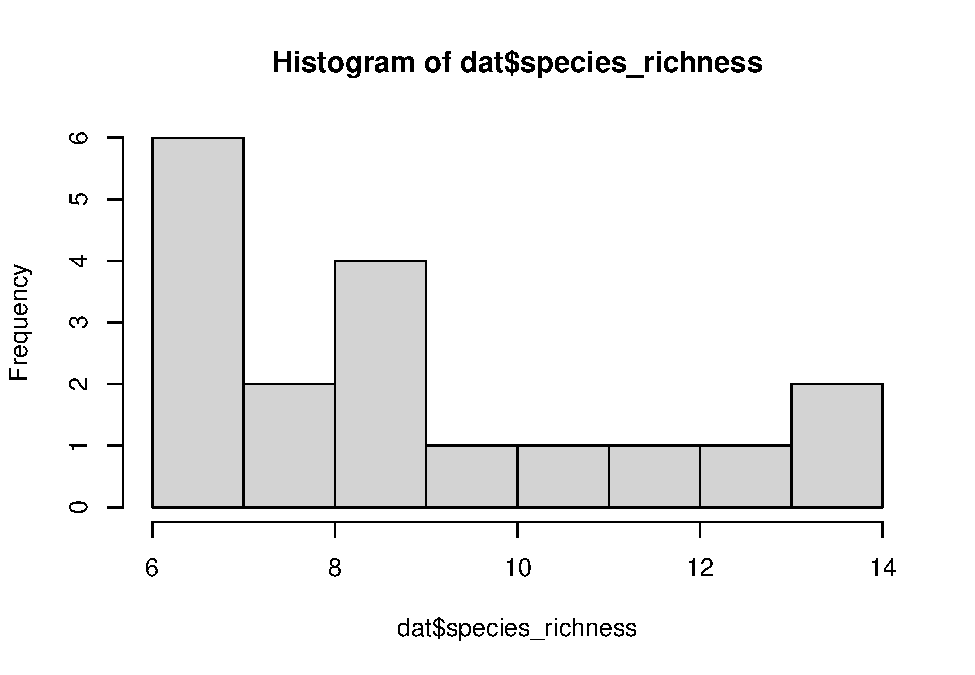
\includegraphics{birdsdataanalysis_files/figure-latex/unnamed-chunk-5-1.pdf}

\begin{Shaded}
\begin{Highlighting}[]
\FunctionTok{kruskal.test}\NormalTok{(dat}\SpecialCharTok{$}\NormalTok{species\_richness, dat}\SpecialCharTok{$}\NormalTok{category) }\CommentTok{\#p{-}value = 0.01533}
\end{Highlighting}
\end{Shaded}

\begin{verbatim}
## 
##  Kruskal-Wallis rank sum test
## 
## data:  dat$species_richness and dat$category
## Kruskal-Wallis chi-squared = 5.8783, df = 1, p-value = 0.01533
\end{verbatim}

\begin{Shaded}
\begin{Highlighting}[]
\FunctionTok{boxplot}\NormalTok{(species\_richness}\SpecialCharTok{\textasciitilde{}}\NormalTok{category, }\AttributeTok{data=}\NormalTok{dat, }\AttributeTok{xlab=} \StringTok{"Category"}\NormalTok{, }\AttributeTok{ylab=} \StringTok{"Species richness"}\NormalTok{, }\AttributeTok{col=} \FunctionTok{c}\NormalTok{(}\StringTok{"lightgreen"}\NormalTok{, }\StringTok{"lightblue"}\NormalTok{))}
\FunctionTok{text}\NormalTok{(}\DecValTok{1}\NormalTok{,}\FloatTok{13.6}\NormalTok{,}\AttributeTok{labels =} \StringTok{"p{-}value: 0.015"}\NormalTok{, }\AttributeTok{cex =} \DecValTok{1}\NormalTok{)}
\end{Highlighting}
\end{Shaded}

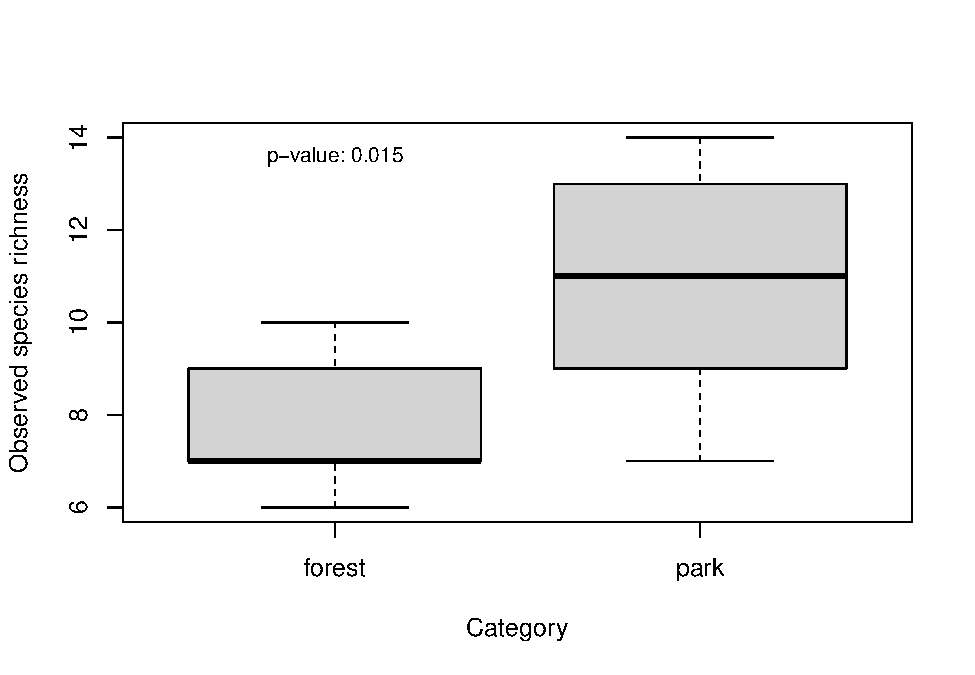
\includegraphics{birdsdataanalysis_files/figure-latex/unnamed-chunk-5-2.pdf}

\begin{Shaded}
\begin{Highlighting}[]
\FunctionTok{hist}\NormalTok{(dat}\SpecialCharTok{$}\NormalTok{species\_abund) }\CommentTok{\# not normally distributed}
\end{Highlighting}
\end{Shaded}

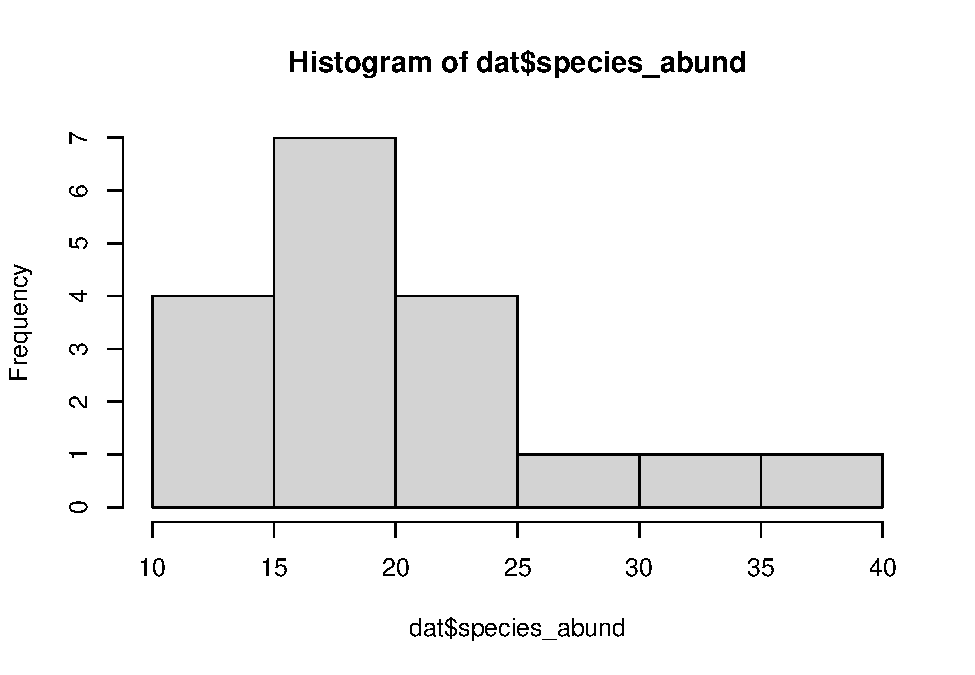
\includegraphics{birdsdataanalysis_files/figure-latex/unnamed-chunk-5-3.pdf}

\begin{Shaded}
\begin{Highlighting}[]
\FunctionTok{kruskal.test}\NormalTok{(dat}\SpecialCharTok{$}\NormalTok{species\_abund, dat}\SpecialCharTok{$}\NormalTok{category) }\CommentTok{\#p{-}value = 0.0046}
\end{Highlighting}
\end{Shaded}

\begin{verbatim}
## 
##  Kruskal-Wallis rank sum test
## 
## data:  dat$species_abund and dat$category
## Kruskal-Wallis chi-squared = 8.0175, df = 1, p-value = 0.004633
\end{verbatim}

\begin{Shaded}
\begin{Highlighting}[]
\FunctionTok{boxplot}\NormalTok{(species\_abund}\SpecialCharTok{\textasciitilde{}}\NormalTok{category, }\AttributeTok{data=}\NormalTok{dat, }\AttributeTok{xlab=} \StringTok{"Category"}\NormalTok{, }\AttributeTok{ylab=} \StringTok{"Species abundance"}\NormalTok{, }\AttributeTok{col=} \FunctionTok{c}\NormalTok{(}\StringTok{"lightgreen"}\NormalTok{, }\StringTok{"lightblue"}\NormalTok{))}
\FunctionTok{text}\NormalTok{(}\DecValTok{1}\NormalTok{,}\DecValTok{35}\NormalTok{,}\AttributeTok{labels =} \StringTok{"p{-}value: 0.005"}\NormalTok{, }\AttributeTok{cex =} \DecValTok{1}\NormalTok{)}
\end{Highlighting}
\end{Shaded}

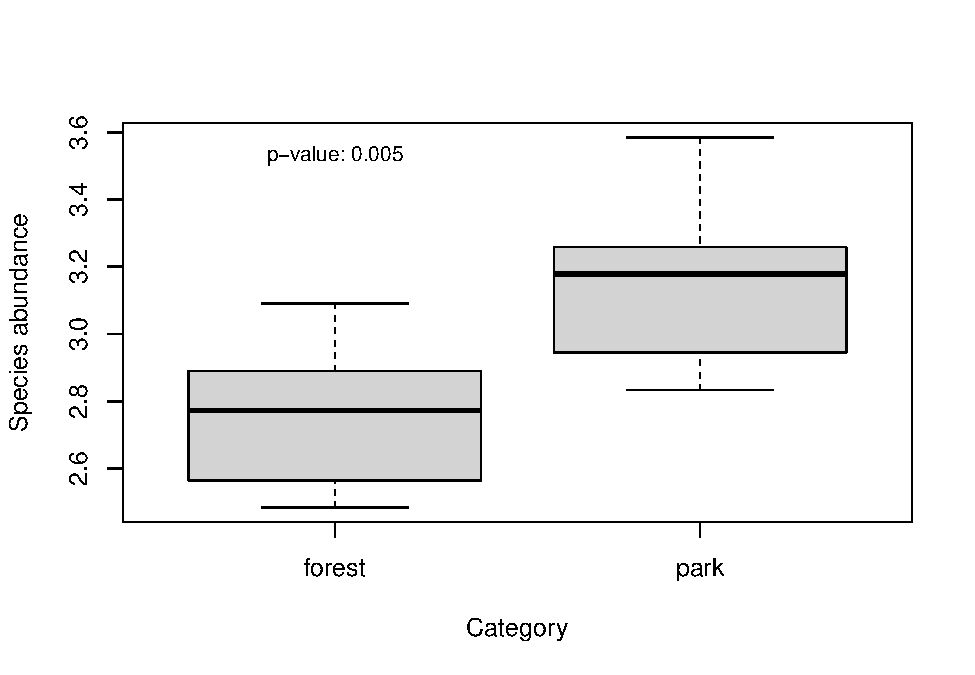
\includegraphics{birdsdataanalysis_files/figure-latex/unnamed-chunk-5-4.pdf}

\begin{Shaded}
\begin{Highlighting}[]
\FunctionTok{hist}\NormalTok{(dat}\SpecialCharTok{$}\NormalTok{rarefied\_richness) }\CommentTok{\# normally distributed}
\end{Highlighting}
\end{Shaded}

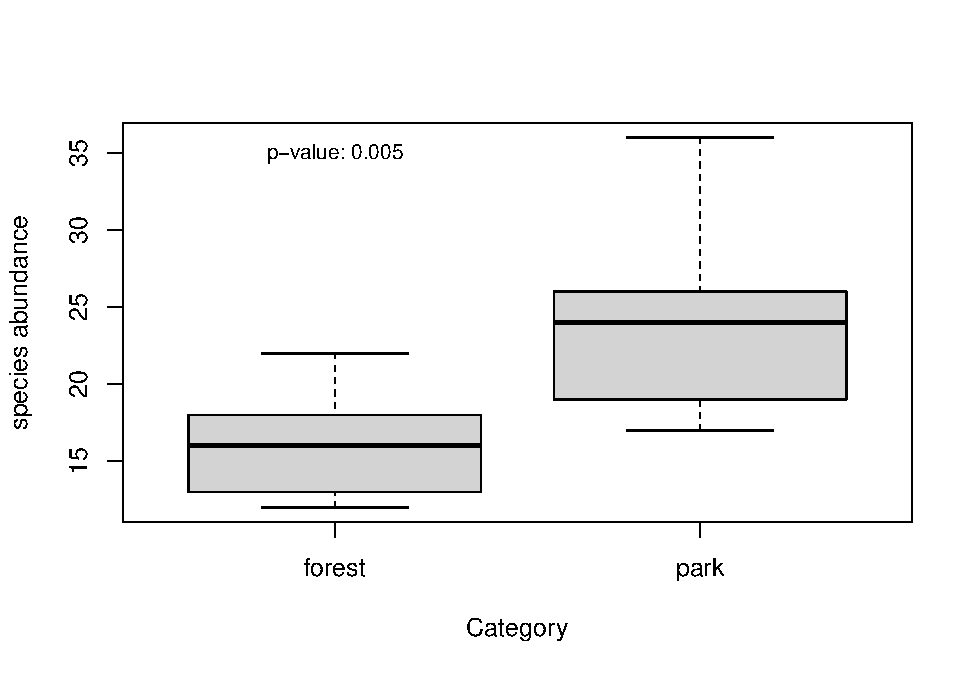
\includegraphics{birdsdataanalysis_files/figure-latex/unnamed-chunk-5-5.pdf}

\begin{Shaded}
\begin{Highlighting}[]
\NormalTok{mod}\OtherTok{\textless{}{-}}\FunctionTok{aov}\NormalTok{(dat}\SpecialCharTok{$}\NormalTok{rarefied\_richness }\SpecialCharTok{\textasciitilde{}}\NormalTok{ dat}\SpecialCharTok{$}\NormalTok{category)}
\FunctionTok{summary}\NormalTok{(mod) }\CommentTok{\#p{-}value: 0.291}
\end{Highlighting}
\end{Shaded}

\begin{verbatim}
##              Df Sum Sq Mean Sq F value Pr(>F)
## dat$category  1  0.941  0.9405   1.194  0.291
## Residuals    16 12.605  0.7878
\end{verbatim}

\begin{Shaded}
\begin{Highlighting}[]
\FunctionTok{boxplot}\NormalTok{(rarefied\_richness}\SpecialCharTok{\textasciitilde{}}\NormalTok{category, }\AttributeTok{data=}\NormalTok{dat, }\AttributeTok{xlab=} \StringTok{"Category"}\NormalTok{, }\AttributeTok{ylab=} \StringTok{"Rarefied richness"}\NormalTok{, }\AttributeTok{col=} \FunctionTok{c}\NormalTok{(}\StringTok{"lightgreen"}\NormalTok{, }\StringTok{"lightblue"}\NormalTok{))}
\FunctionTok{text}\NormalTok{(}\DecValTok{1}\NormalTok{,}\FloatTok{5.5}\NormalTok{,}\AttributeTok{labels =} \StringTok{"p{-}value: 0.291"}\NormalTok{, }\AttributeTok{cex =} \DecValTok{1}\NormalTok{)}
\end{Highlighting}
\end{Shaded}

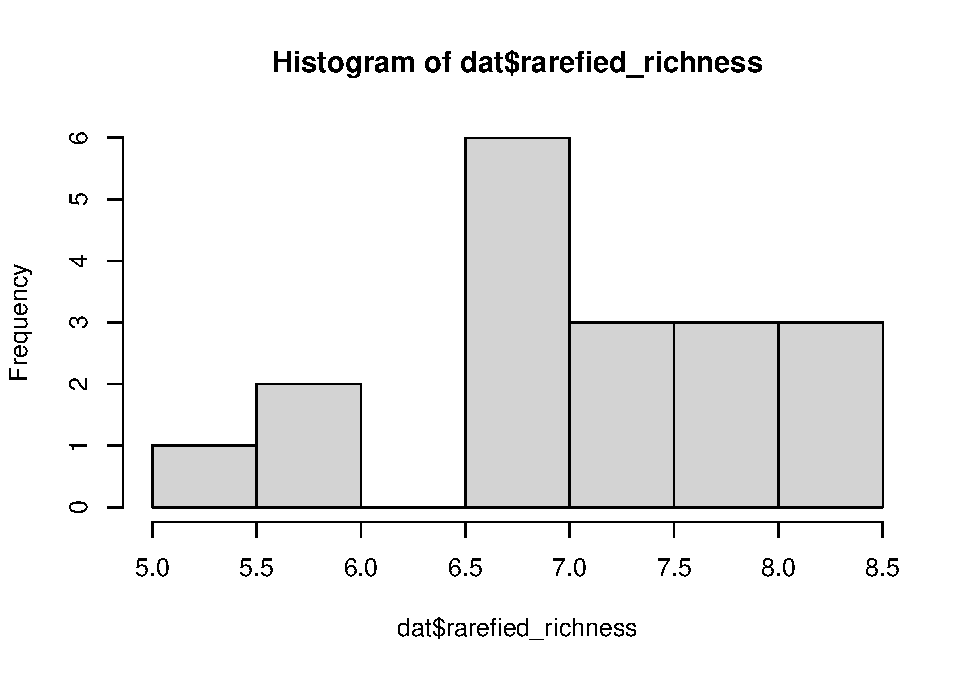
\includegraphics{birdsdataanalysis_files/figure-latex/unnamed-chunk-5-6.pdf}

\begin{Shaded}
\begin{Highlighting}[]
\FunctionTok{layout}\NormalTok{(}\FunctionTok{matrix}\NormalTok{(}\FunctionTok{c}\NormalTok{(}\DecValTok{1}\SpecialCharTok{:}\DecValTok{4}\NormalTok{), }\AttributeTok{nrow=}\DecValTok{2}\NormalTok{, }\AttributeTok{byrow=}\ConstantTok{FALSE}\NormalTok{))}
\FunctionTok{boxplot}\NormalTok{(species\_richness}\SpecialCharTok{\textasciitilde{}}\NormalTok{category, }\AttributeTok{data=}\NormalTok{dat, }\AttributeTok{xlab=} \StringTok{"Category"}\NormalTok{, }\AttributeTok{ylab=} \StringTok{"Species richness"}\NormalTok{)}
\FunctionTok{boxplot}\NormalTok{(}\FunctionTok{log}\NormalTok{(species\_abund}\SpecialCharTok{+}\DecValTok{1}\NormalTok{)}\SpecialCharTok{\textasciitilde{}}\NormalTok{category, }\AttributeTok{data=}\NormalTok{dat, }\AttributeTok{xlab=} \StringTok{"Category"}\NormalTok{, }\AttributeTok{ylab=} \StringTok{"Species abundance"}\NormalTok{)}
\CommentTok{\#?boxplot}
\FunctionTok{boxplot}\NormalTok{(rarefied\_richness}\SpecialCharTok{\textasciitilde{}}\NormalTok{category, }\AttributeTok{data=}\NormalTok{dat, }\AttributeTok{xlab=} \StringTok{"Category"}\NormalTok{, }\AttributeTok{ylab=} \StringTok{"Rarefied richness"}\NormalTok{)}
\FunctionTok{layout}\NormalTok{(}\FunctionTok{matrix}\NormalTok{(}\FunctionTok{c}\NormalTok{(}\DecValTok{1}\SpecialCharTok{:}\DecValTok{4}\NormalTok{), }\AttributeTok{nrow=}\DecValTok{2}\NormalTok{, }\AttributeTok{byrow=}\ConstantTok{FALSE}\NormalTok{))}
\end{Highlighting}
\end{Shaded}

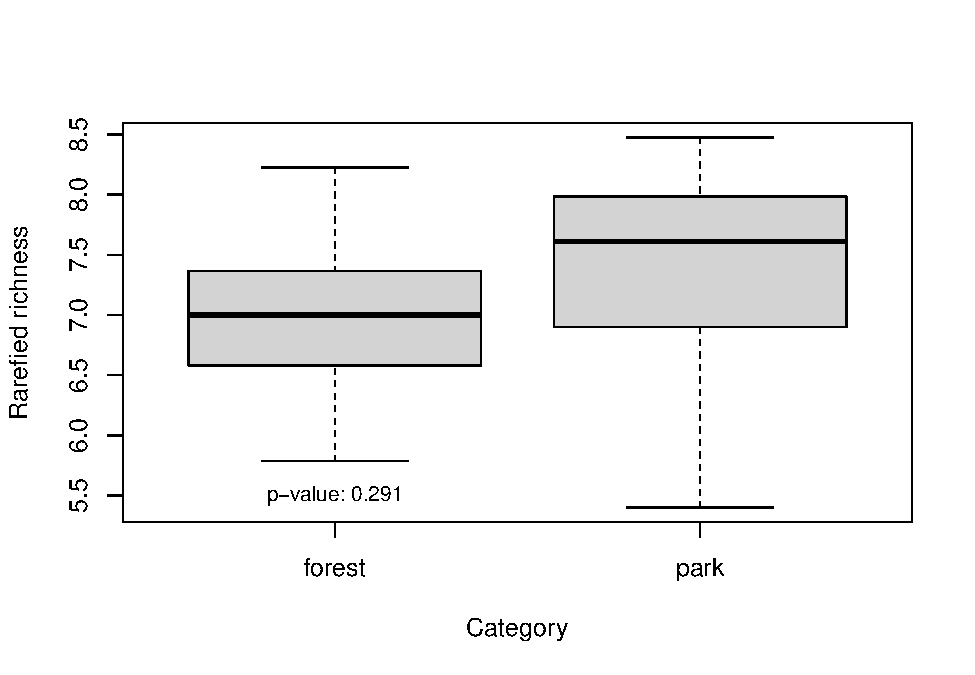
\includegraphics{birdsdataanalysis_files/figure-latex/unnamed-chunk-5-7.pdf}

\begin{Shaded}
\begin{Highlighting}[]
\FunctionTok{boxplot}\NormalTok{(species\_richness}\SpecialCharTok{\textasciitilde{}}\NormalTok{category, }\AttributeTok{data=}\NormalTok{dat, }\AttributeTok{xlab=} \StringTok{"Category"}\NormalTok{, }\AttributeTok{ylab=} \StringTok{"Species richness"}\NormalTok{, }\AttributeTok{col=} \FunctionTok{c}\NormalTok{(}\StringTok{"lightgreen"}\NormalTok{, }\StringTok{"lightblue"}\NormalTok{))}
\FunctionTok{boxplot}\NormalTok{(}\FunctionTok{log}\NormalTok{(species\_abund}\SpecialCharTok{+}\DecValTok{1}\NormalTok{)}\SpecialCharTok{\textasciitilde{}}\NormalTok{category, }\AttributeTok{data=}\NormalTok{dat, }\AttributeTok{xlab=} \StringTok{"Category"}\NormalTok{, }\AttributeTok{ylab=} \StringTok{"Species abundance"}\NormalTok{, }\AttributeTok{col=} \FunctionTok{c}\NormalTok{(}\StringTok{"lightgreen"}\NormalTok{, }\StringTok{"lightblue"}\NormalTok{))}
\CommentTok{\#?boxplot}
\FunctionTok{boxplot}\NormalTok{(rarefied\_richness}\SpecialCharTok{\textasciitilde{}}\NormalTok{category, }\AttributeTok{data=}\NormalTok{dat, }\AttributeTok{xlab=} \StringTok{"Category"}\NormalTok{, }\AttributeTok{ylab=} \StringTok{"Rarefied richness"}\NormalTok{, }\AttributeTok{col=} \FunctionTok{c}\NormalTok{(}\StringTok{"lightgreen"}\NormalTok{, }\StringTok{"lightblue"}\NormalTok{))}
\end{Highlighting}
\end{Shaded}

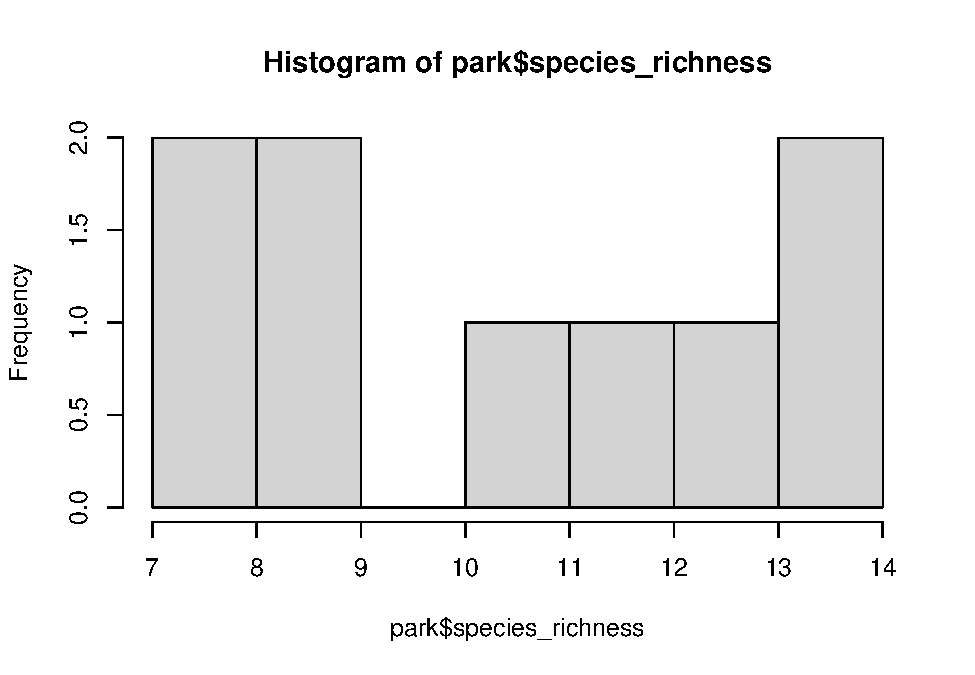
\includegraphics{birdsdataanalysis_files/figure-latex/unnamed-chunk-5-8.pdf}

\begin{Shaded}
\begin{Highlighting}[]
\FunctionTok{boxplot}\NormalTok{(species\_richness}\SpecialCharTok{\textasciitilde{}}\NormalTok{category, }\AttributeTok{data=}\NormalTok{dat, }\AttributeTok{xlab=} \StringTok{"Category"}\NormalTok{, }\AttributeTok{ylab=} \StringTok{"Species richness"}\NormalTok{)}
\end{Highlighting}
\end{Shaded}

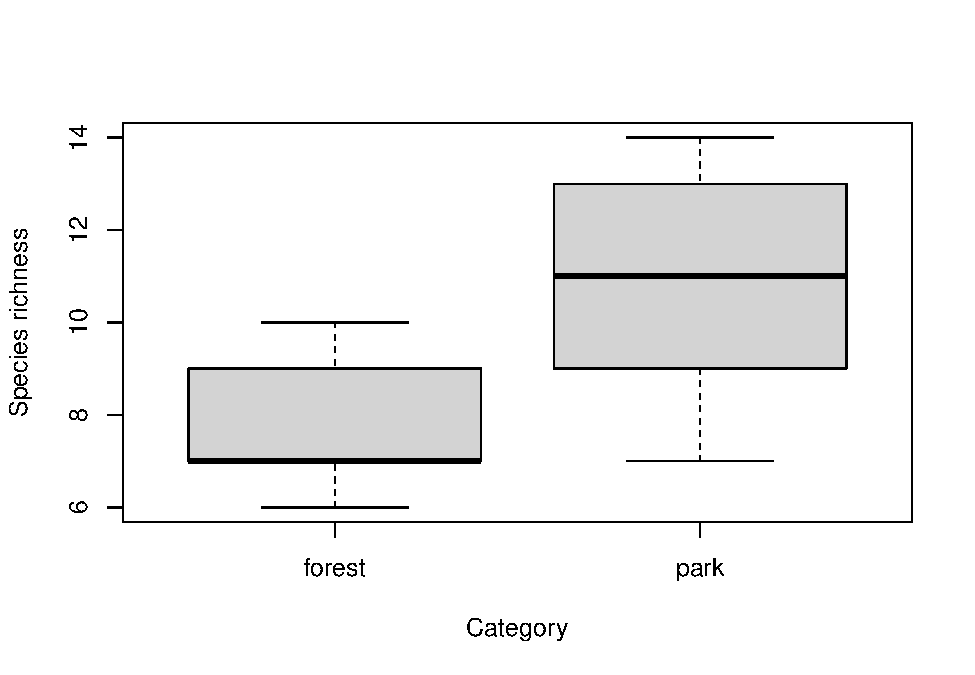
\includegraphics{birdsdataanalysis_files/figure-latex/unnamed-chunk-6-1.pdf}

\begin{Shaded}
\begin{Highlighting}[]
\FunctionTok{boxplot}\NormalTok{(}\FunctionTok{log}\NormalTok{(species\_abund}\SpecialCharTok{+}\DecValTok{1}\NormalTok{)}\SpecialCharTok{\textasciitilde{}}\NormalTok{category, }\AttributeTok{data=}\NormalTok{dat, }\AttributeTok{xlab=} \StringTok{"Category"}\NormalTok{, }\AttributeTok{ylab=} \StringTok{"Species abundance"}\NormalTok{)}
\end{Highlighting}
\end{Shaded}

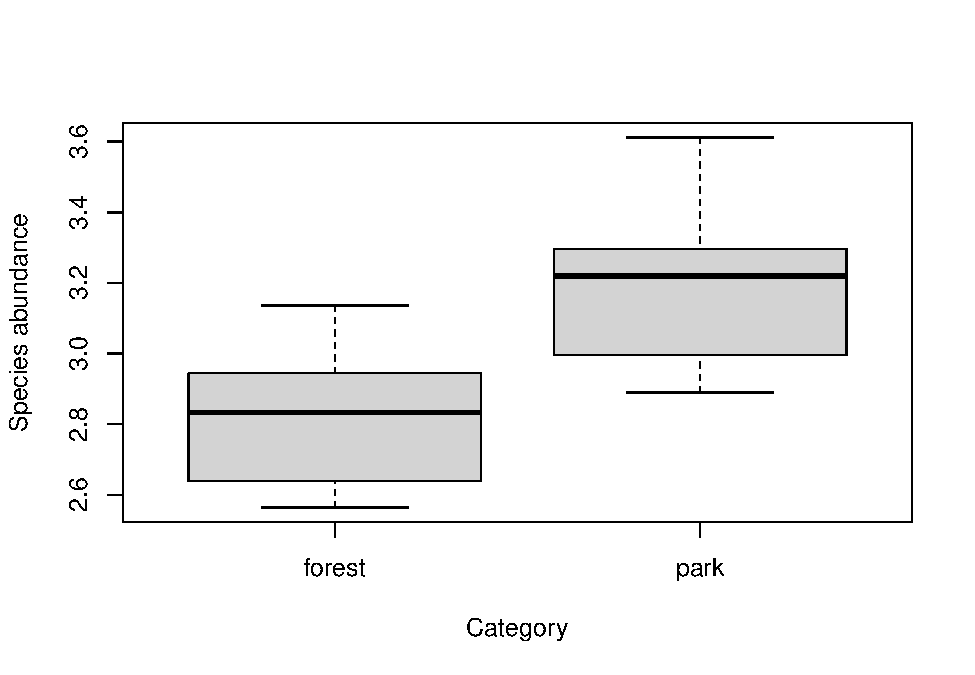
\includegraphics{birdsdataanalysis_files/figure-latex/unnamed-chunk-6-2.pdf}

\begin{Shaded}
\begin{Highlighting}[]
\CommentTok{\#?boxplot}
\FunctionTok{boxplot}\NormalTok{(rarefied\_richness}\SpecialCharTok{\textasciitilde{}}\NormalTok{category, }\AttributeTok{data=}\NormalTok{dat, }\AttributeTok{xlab=} \StringTok{"Category"}\NormalTok{, }\AttributeTok{ylab=} \StringTok{"Rarefied richness"}\NormalTok{)}
\end{Highlighting}
\end{Shaded}

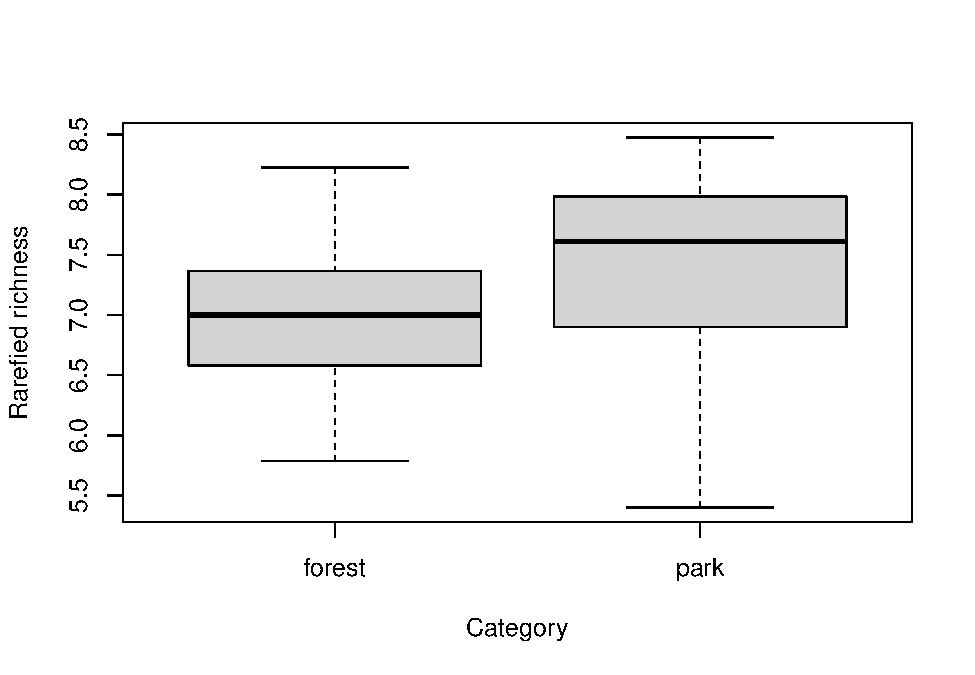
\includegraphics{birdsdataanalysis_files/figure-latex/unnamed-chunk-6-3.pdf}

\begin{Shaded}
\begin{Highlighting}[]
\FunctionTok{boxplot}\NormalTok{(species\_richness}\SpecialCharTok{\textasciitilde{}}\NormalTok{category, }\AttributeTok{data=}\NormalTok{dat, }\AttributeTok{xlab=} \StringTok{"Category"}\NormalTok{, }\AttributeTok{ylab=} \StringTok{"Species richness"}\NormalTok{, }\AttributeTok{col=} \FunctionTok{c}\NormalTok{(}\StringTok{"lightgreen"}\NormalTok{, }\StringTok{"lightblue"}\NormalTok{))}
\end{Highlighting}
\end{Shaded}

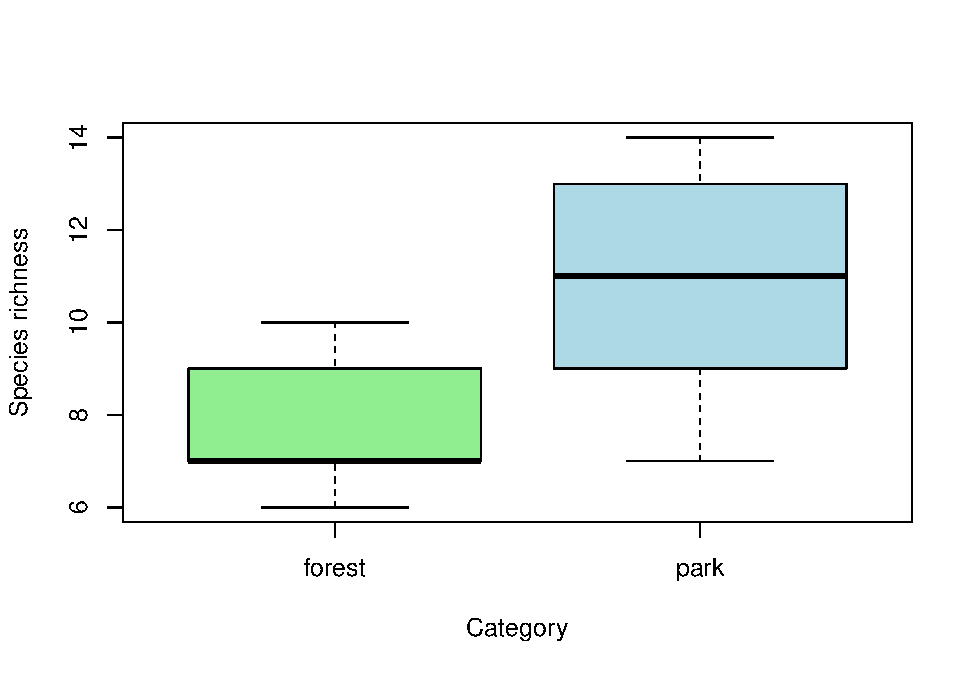
\includegraphics{birdsdataanalysis_files/figure-latex/unnamed-chunk-6-4.pdf}

\begin{Shaded}
\begin{Highlighting}[]
\FunctionTok{boxplot}\NormalTok{(}\FunctionTok{log}\NormalTok{(species\_abund}\SpecialCharTok{+}\DecValTok{1}\NormalTok{)}\SpecialCharTok{\textasciitilde{}}\NormalTok{category, }\AttributeTok{data=}\NormalTok{dat, }\AttributeTok{xlab=} \StringTok{"Category"}\NormalTok{, }\AttributeTok{ylab=} \StringTok{"Species abundance"}\NormalTok{, }\AttributeTok{col=} \FunctionTok{c}\NormalTok{(}\StringTok{"lightgreen"}\NormalTok{, }\StringTok{"lightblue"}\NormalTok{))}
\end{Highlighting}
\end{Shaded}

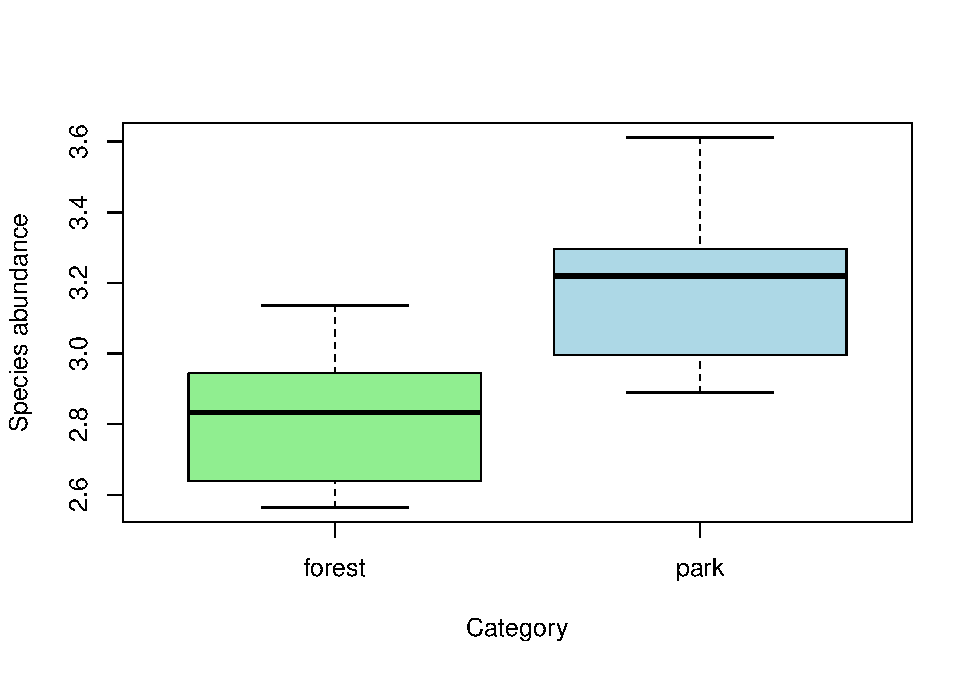
\includegraphics{birdsdataanalysis_files/figure-latex/unnamed-chunk-6-5.pdf}

\begin{Shaded}
\begin{Highlighting}[]
\CommentTok{\#?boxplot}
\FunctionTok{boxplot}\NormalTok{(rarefied\_richness}\SpecialCharTok{\textasciitilde{}}\NormalTok{category, }\AttributeTok{data=}\NormalTok{dat, }\AttributeTok{xlab=} \StringTok{"Category"}\NormalTok{, }\AttributeTok{ylab=} \StringTok{"Rarefied richness"}\NormalTok{, }\AttributeTok{col=} \FunctionTok{c}\NormalTok{(}\StringTok{"lightgreen"}\NormalTok{, }\StringTok{"lightblue"}\NormalTok{))}
\end{Highlighting}
\end{Shaded}

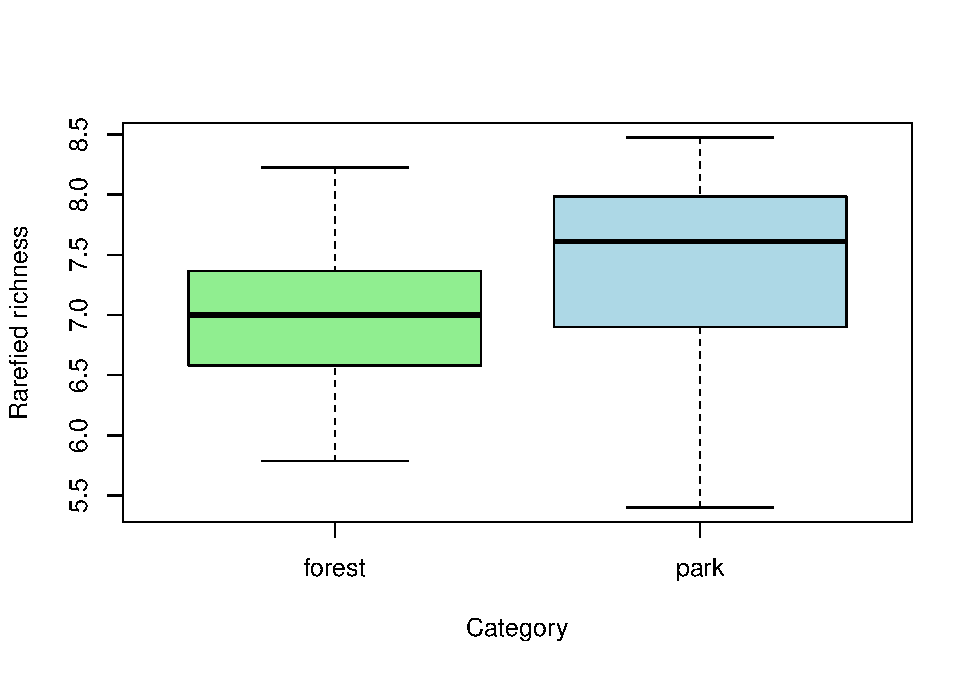
\includegraphics{birdsdataanalysis_files/figure-latex/unnamed-chunk-6-6.pdf}

\#\#Now let's begin with the data analysis

\#2a linear models: to check for difference between habitat types with
the implementation of mixed effect models.

\begin{Shaded}
\begin{Highlighting}[]
\NormalTok{mod1 }\OtherTok{\textless{}{-}} \FunctionTok{lme}\NormalTok{(species\_richness}\SpecialCharTok{\textasciitilde{}}\NormalTok{category, }\AttributeTok{random =}\NormalTok{ (}\SpecialCharTok{\textasciitilde{}}\DecValTok{1}\SpecialCharTok{|}\NormalTok{site), }\AttributeTok{data=}\NormalTok{dat) }\CommentTok{\#model structure, random=... specifies how the data are structured (subsamples nested in study site)}
\FunctionTok{summary}\NormalTok{(mod1) }\CommentTok{\#model output {-} important is the "fixed effects" part. Here "forest" is hiding in the "Intercept" and the categorypark{-}row is showing the difference between park and forest}
\end{Highlighting}
\end{Shaded}

\begin{verbatim}
## Linear mixed-effects model fit by REML
##   Data: dat 
##        AIC     BIC    logLik
##   78.65584 81.7462 -35.32792
## 
## Random effects:
##  Formula: ~1 | site
##         (Intercept) Residual
## StdDev:    1.459325 1.649916
## 
## Fixed effects:  species_richness ~ category 
##                 Value Std.Error DF  t-value p-value
## (Intercept)  7.777778  1.006154 12 7.730207  0.0000
## categorypark 3.000000  1.422916  4 2.108346  0.1027
##  Correlation: 
##              (Intr)
## categorypark -0.707
## 
## Standardized Within-Group Residuals:
##        Min         Q1        Med         Q3        Max 
## -1.5969444 -0.5205776 -0.1919700  0.8175666  1.4335132 
## 
## Number of Observations: 18
## Number of Groups: 6
\end{verbatim}

\begin{Shaded}
\begin{Highlighting}[]
\FunctionTok{plot}\NormalTok{(mod1) }\CommentTok{\#check for homogeneity of variances (data points should have similar vertical spread along the x{-}axis)}
\end{Highlighting}
\end{Shaded}

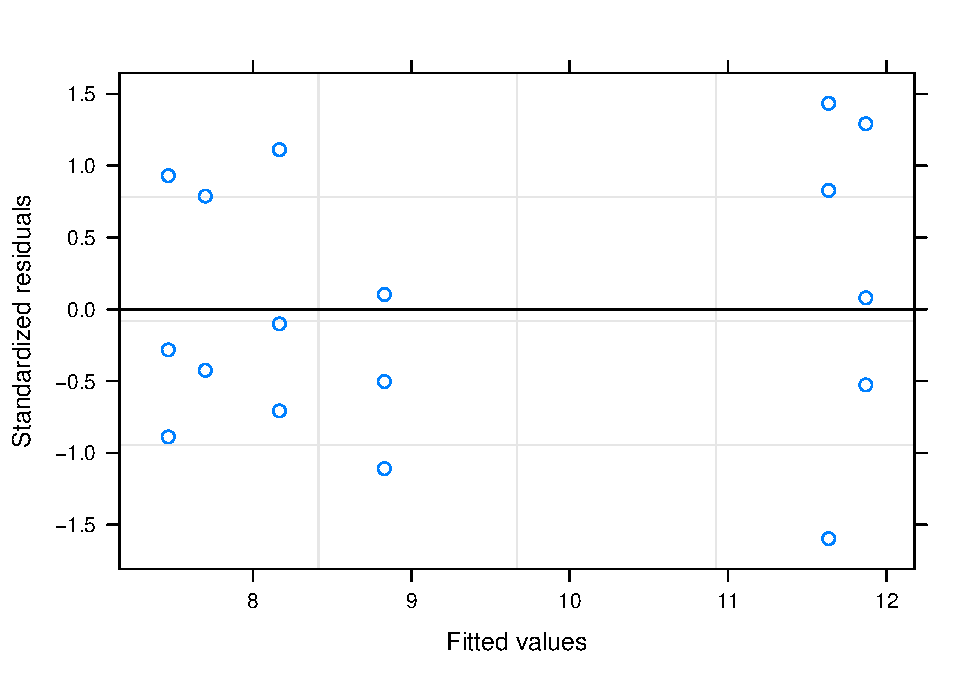
\includegraphics{birdsdataanalysis_files/figure-latex/unnamed-chunk-7-1.pdf}

\begin{Shaded}
\begin{Highlighting}[]
\FunctionTok{qqnorm}\NormalTok{(mod1, }\SpecialCharTok{\textasciitilde{}}\FunctionTok{resid}\NormalTok{(.,}\AttributeTok{type=}\StringTok{"p"}\NormalTok{), }\AttributeTok{abline =} \FunctionTok{c}\NormalTok{(}\DecValTok{0}\NormalTok{,}\DecValTok{1}\NormalTok{)) }\CommentTok{\#check for normality of residuals (should not be completely off the line)}
\end{Highlighting}
\end{Shaded}

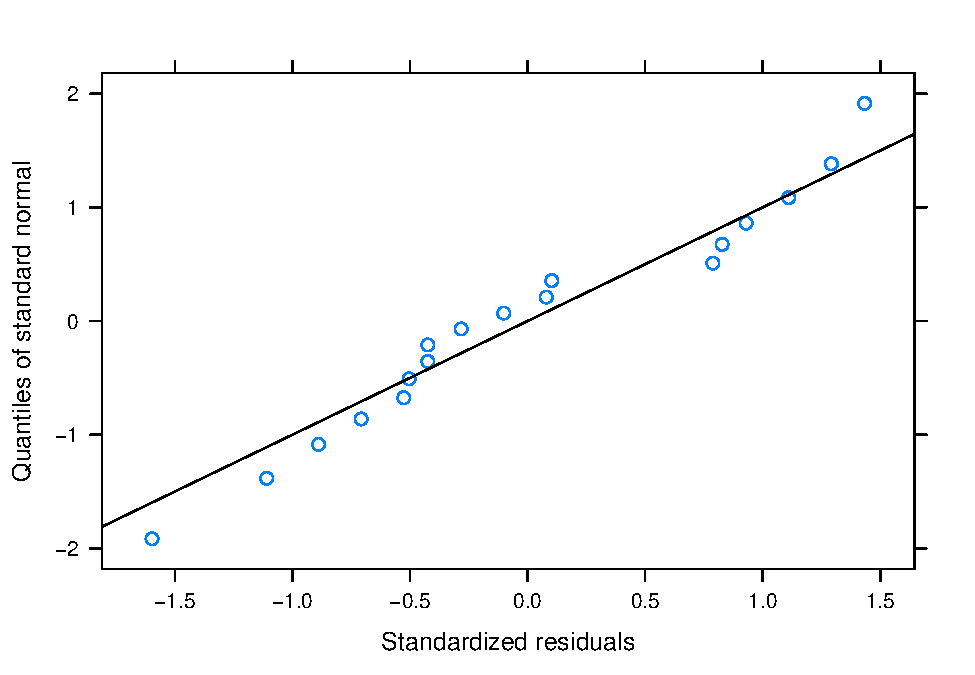
\includegraphics{birdsdataanalysis_files/figure-latex/unnamed-chunk-7-2.pdf}

\#2b linear models to include environmental variables and see the
variation of the data with each of them.

\begin{Shaded}
\begin{Highlighting}[]
\DocumentationTok{\#\#\# MIXED EFFECTS MODEL WITH SPECIES RICHNESS}

\FunctionTok{round}\NormalTok{(}\FunctionTok{cor}\NormalTok{(dat[,}\DecValTok{32}\SpecialCharTok{:}\DecValTok{45}\NormalTok{]),}\DecValTok{2}\NormalTok{) }\CommentTok{\#check which predictor variables are strongly correlated (below {-}0.7 or above 0.7) {-} highly correlated variables should not be included together in the same model (select only one of them, e.g. the one more strongly related to the response variable)}
\end{Highlighting}
\end{Shaded}

\begin{verbatim}
##                 canopy_cover n_tree_spec n_tree_ind dbh_min dbh_min5 dbh_mean
## canopy_cover            1.00       -0.68       0.22   -0.43    -0.38    -0.42
## n_tree_spec            -0.68        1.00      -0.42    0.30     0.18     0.31
## n_tree_ind              0.22       -0.42       1.00   -0.12    -0.51    -0.49
## dbh_min                -0.43        0.30      -0.12    1.00     0.37     0.68
## dbh_min5               -0.38        0.18      -0.51    0.37     1.00     0.71
## dbh_mean               -0.42        0.31      -0.49    0.68     0.71     1.00
## dbh_max                -0.33        0.23      -0.52    0.26     0.57     0.83
## dbh_median             -0.29        0.29      -0.56    0.30     0.89     0.74
## dbh_sd                 -0.69        0.78      -0.63    0.09     0.39     0.36
## n_microhabitats         0.30       -0.42      -0.12   -0.06     0.44     0.27
## latitude                0.30       -0.60       0.22   -0.23     0.04    -0.08
## longitude               0.71       -0.64       0.32   -0.57    -0.50    -0.42
## size                    0.64       -0.52       0.35   -0.33    -0.55    -0.52
## temperature            -0.02        0.03       0.44   -0.29    -0.49    -0.26
##                 dbh_max dbh_median dbh_sd n_microhabitats latitude longitude
## canopy_cover      -0.33      -0.29  -0.69            0.30     0.30      0.71
## n_tree_spec        0.23       0.29   0.78           -0.42    -0.60     -0.64
## n_tree_ind        -0.52      -0.56  -0.63           -0.12     0.22      0.32
## dbh_min            0.26       0.30   0.09           -0.06    -0.23     -0.57
## dbh_min5           0.57       0.89   0.39            0.44     0.04     -0.50
## dbh_mean           0.83       0.74   0.36            0.27    -0.08     -0.42
## dbh_max            1.00       0.57   0.47            0.14     0.03     -0.19
## dbh_median         0.57       1.00   0.44            0.49    -0.06     -0.39
## dbh_sd             0.47       0.44   1.00           -0.32    -0.40     -0.58
## n_microhabitats    0.14       0.49  -0.32            1.00     0.30      0.21
## latitude           0.03      -0.06  -0.40            0.30     1.00      0.14
## longitude         -0.19      -0.39  -0.58            0.21     0.14      1.00
## size              -0.52      -0.48  -0.61            0.22    -0.09      0.80
## temperature       -0.06      -0.38  -0.02           -0.45     0.05      0.23
##                  size temperature
## canopy_cover     0.64       -0.02
## n_tree_spec     -0.52        0.03
## n_tree_ind       0.35        0.44
## dbh_min         -0.33       -0.29
## dbh_min5        -0.55       -0.49
## dbh_mean        -0.52       -0.26
## dbh_max         -0.52       -0.06
## dbh_median      -0.48       -0.38
## dbh_sd          -0.61       -0.02
## n_microhabitats  0.22       -0.45
## latitude        -0.09        0.05
## longitude        0.80        0.23
## size             1.00       -0.07
## temperature     -0.07        1.00
\end{verbatim}

\begin{Shaded}
\begin{Highlighting}[]
\NormalTok{mod2 }\OtherTok{\textless{}{-}} \FunctionTok{lme}\NormalTok{(species\_richness }\SpecialCharTok{\textasciitilde{}}\NormalTok{ category}\SpecialCharTok{*}\NormalTok{size }\SpecialCharTok{+}\NormalTok{ canopy\_cover }\SpecialCharTok{+}\NormalTok{ n\_tree\_spec }\SpecialCharTok{+}\NormalTok{ n\_tree\_ind }\SpecialCharTok{+}\NormalTok{ dbh\_mean }\SpecialCharTok{+}\NormalTok{ n\_microhabitats }\SpecialCharTok{+}\NormalTok{ temperature, }\AttributeTok{random =}\NormalTok{ (}\SpecialCharTok{\textasciitilde{}}\DecValTok{1}\SpecialCharTok{|}\NormalTok{site), }\AttributeTok{data=}\NormalTok{dat, }\AttributeTok{method=}\StringTok{"ML"}\NormalTok{) }\CommentTok{\#initial, full model with all potential predictor variables}
\FunctionTok{summary}\NormalTok{(mod2)}
\end{Highlighting}
\end{Shaded}

\begin{verbatim}
## Linear mixed-effects model fit by maximum likelihood
##   Data: dat 
##        AIC      BIC    logLik
##   78.15111 88.83557 -27.07555
## 
## Random effects:
##  Formula: ~1 | site
##          (Intercept) Residual
## StdDev: 2.203848e-05 1.088999
## 
## Fixed effects:  species_richness ~ category * size + canopy_cover + n_tree_spec +      n_tree_ind + dbh_mean + n_microhabitats + temperature 
##                       Value Std.Error DF   t-value p-value
## (Intercept)       15.944431  4.962963  7  3.212684  0.0148
## categorypark      -0.929198  2.765989  1 -0.335937  0.7937
## size              -0.004414  0.011233  1 -0.392967  0.7616
## canopy_cover      -0.043150  0.026056  7 -1.656089  0.1417
## n_tree_spec       -0.396169  0.318390  7 -1.244288  0.2534
## n_tree_ind         0.015184  0.153805  7  0.098722  0.9241
## dbh_mean           0.054217  0.028035  7  1.933885  0.0944
## n_microhabitats   -0.071704  0.088881  7 -0.806747  0.4464
## temperature       -0.262180  0.164449  1 -1.594289  0.3566
## categorypark:size  0.065564  0.053671  1  1.221589  0.4367
##  Correlation: 
##                   (Intr) ctgryp size   cnpy_c n_tr_s n_tr_n dbh_mn n_mcrh
## categorypark      -0.450                                                 
## size              -0.383  0.726                                          
## canopy_cover      -0.622  0.338  0.026                                   
## n_tree_spec       -0.316 -0.403 -0.319  0.131                            
## n_tree_ind        -0.497  0.146 -0.036  0.142  0.430                     
## dbh_mean          -0.151 -0.473 -0.134  0.020  0.173  0.126              
## n_microhabitats   -0.304  0.196  0.084  0.068  0.013 -0.148 -0.412       
## temperature       -0.306  0.294  0.358  0.148 -0.408 -0.528 -0.126  0.504
## categorypark:size -0.004 -0.164 -0.054  0.196 -0.348 -0.514  0.102  0.324
##                   tmprtr
## categorypark            
## size                    
## canopy_cover            
## n_tree_spec             
## n_tree_ind              
## dbh_mean                
## n_microhabitats         
## temperature             
## categorypark:size  0.544
## 
## Standardized Within-Group Residuals:
##        Min         Q1        Med         Q3        Max 
## -1.7168405 -0.6187248 -0.1021469  0.7833831  2.2863006 
## 
## Number of Observations: 18
## Number of Groups: 6
\end{verbatim}

\begin{Shaded}
\begin{Highlighting}[]
\NormalTok{mod2}\FloatTok{.1} \OtherTok{\textless{}{-}} \FunctionTok{stepAIC}\NormalTok{(mod2) }\CommentTok{\#model simplification based on AIC{-}value of the model}
\end{Highlighting}
\end{Shaded}

\begin{verbatim}
## Start:  AIC=78.15
## species_richness ~ category * size + canopy_cover + n_tree_spec + 
##     n_tree_ind + dbh_mean + n_microhabitats + temperature
## 
##                   Df    AIC
## - n_tree_ind       1 76.173
## - n_microhabitats  1 77.559
## <none>               78.151
## - category:size    1 79.230
## - n_tree_spec      1 79.336
## - temperature      1 81.117
## - canopy_cover     1 81.457
## - dbh_mean         1 83.055
## 
## Step:  AIC=76.17
## species_richness ~ category + size + canopy_cover + n_tree_spec + 
##     dbh_mean + n_microhabitats + temperature + category:size
## 
##                   Df    AIC
## - n_microhabitats  1 75.560
## <none>               76.173
## - n_tree_spec      1 78.242
## - category:size    1 78.540
## - canopy_cover     1 79.647
## - temperature      1 80.376
## - dbh_mean         1 81.088
## 
## Step:  AIC=75.56
## species_richness ~ category + size + canopy_cover + n_tree_spec + 
##     dbh_mean + temperature + category:size
## 
##                 Df    AIC
## <none>             75.560
## - n_tree_spec    1 77.056
## - canopy_cover   1 78.333
## - temperature    1 78.407
## - dbh_mean       1 79.089
## - category:size  1 79.262
\end{verbatim}

\begin{Shaded}
\begin{Highlighting}[]
\FunctionTok{summary}\NormalTok{(mod2}\FloatTok{.1}\NormalTok{) }\CommentTok{\#final model which includes only the most important predictors }
\end{Highlighting}
\end{Shaded}

\begin{verbatim}
## Linear mixed-effects model fit by maximum likelihood
##   Data: dat 
##        AIC      BIC    logLik
##   75.55985 84.46357 -27.77993
## 
## Random effects:
##  Formula: ~1 | site
##          (Intercept) Residual
## StdDev: 2.226226e-05 1.132458
## 
## Fixed effects:  species_richness ~ category + size + canopy_cover + n_tree_spec +      dbh_mean + temperature + category:size 
##                       Value Std.Error DF   t-value p-value
## (Intercept)       14.672137  3.597092  9  4.078889  0.0028
## categorypark      -0.482896  2.481824  1 -0.194573  0.8777
## size              -0.003663  0.010409  1 -0.351878  0.7846
## canopy_cover      -0.041630  0.023889  9 -1.742664  0.1154
## n_tree_spec       -0.390018  0.266364  9 -1.464233  0.1772
## dbh_mean           0.044942  0.023700  9  1.896307  0.0904
## temperature       -0.196868  0.111988  1 -1.757941  0.3293
## categorypark:size  0.079072  0.040958  1  1.930546  0.3043
##  Correlation: 
##                   (Intr) ctgryp size   cnpy_c n_tr_s dbh_mn tmprtr
## categorypark      -0.391                                          
## size              -0.477  0.743                                   
## canopy_cover      -0.673  0.312  0.025                            
## n_tree_spec       -0.104 -0.556 -0.345  0.071                     
## dbh_mean          -0.339 -0.461 -0.109  0.043  0.183              
## temperature       -0.708  0.391  0.418  0.255 -0.326  0.168       
## categorypark:size -0.256 -0.183 -0.113  0.305 -0.199  0.357  0.275
## 
## Standardized Within-Group Residuals:
##         Min          Q1         Med          Q3         Max 
## -1.25367764 -1.00232732 -0.09062601  0.80538278  2.22429975 
## 
## Number of Observations: 18
## Number of Groups: 6
\end{verbatim}

\begin{Shaded}
\begin{Highlighting}[]
\NormalTok{mod2}\FloatTok{.2} \OtherTok{\textless{}{-}} \FunctionTok{update}\NormalTok{(mod2}\FloatTok{.1}\NormalTok{, }\SpecialCharTok{\textasciitilde{}}\NormalTok{.}\SpecialCharTok{{-}}\NormalTok{n\_tree\_spec)}
\FunctionTok{summary}\NormalTok{(mod2}\FloatTok{.2}\NormalTok{)}
\end{Highlighting}
\end{Shaded}

\begin{verbatim}
## Linear mixed-effects model fit by maximum likelihood
##   Data: dat 
##        AIC      BIC    logLik
##   77.05632 85.06967 -29.52816
## 
## Random effects:
##  Formula: ~1 | site
##          (Intercept) Residual
## StdDev: 4.567893e-05 1.247966
## 
## Fixed effects:  species_richness ~ category + size + canopy_cover + dbh_mean +      temperature + category:size 
##                       Value Std.Error DF   t-value p-value
## (Intercept)       14.124851  3.759052 10  3.757557  0.0037
## categorypark      -2.502864  2.167710  1 -1.154612  0.4544
## size              -0.008924  0.010265  1 -0.869357  0.5444
## canopy_cover      -0.039147  0.025037 10 -1.563569  0.1490
## dbh_mean           0.051287  0.024482 10  2.094917  0.0626
## temperature       -0.250281  0.111250  1 -2.249714  0.2663
## categorypark:size  0.067136  0.042174  1  1.591857  0.3571
##  Correlation: 
##                   (Intr) ctgryp size   cnpy_c dbh_mn tmprtr
## categorypark      -0.543                                   
## size              -0.550  0.707                            
## canopy_cover      -0.671  0.424  0.052                     
## dbh_mean          -0.327 -0.440 -0.049  0.030              
## temperature       -0.788  0.267  0.344  0.295  0.245       
## categorypark:size -0.284 -0.360 -0.198  0.326  0.409  0.226
## 
## Standardized Within-Group Residuals:
##         Min          Q1         Med          Q3         Max 
## -1.28014570 -0.71138298 -0.04444658  0.61471701  2.93583839 
## 
## Number of Observations: 18
## Number of Groups: 6
\end{verbatim}

\begin{Shaded}
\begin{Highlighting}[]
\FunctionTok{anova}\NormalTok{(mod2}\FloatTok{.1}\NormalTok{, mod2}\FloatTok{.2}\NormalTok{)}
\end{Highlighting}
\end{Shaded}

\begin{verbatim}
##        Model df      AIC      BIC    logLik   Test  L.Ratio p-value
## mod2.1     1 10 75.55985 84.46357 -27.77993                        
## mod2.2     2  9 77.05632 85.06967 -29.52816 1 vs 2 3.496468  0.0615
\end{verbatim}

\begin{Shaded}
\begin{Highlighting}[]
\NormalTok{mod2}\FloatTok{.3} \OtherTok{\textless{}{-}} \FunctionTok{update}\NormalTok{(mod2}\FloatTok{.2}\NormalTok{, }\SpecialCharTok{\textasciitilde{}}\NormalTok{.}\SpecialCharTok{{-}}\NormalTok{temperature)}
\FunctionTok{summary}\NormalTok{(mod2}\FloatTok{.3}\NormalTok{)}
\end{Highlighting}
\end{Shaded}

\begin{verbatim}
## Linear mixed-effects model fit by maximum likelihood
##   Data: dat 
##        AIC      BIC    logLik
##   81.24597 88.36895 -32.62299
## 
## Random effects:
##  Formula: ~1 | site
##         (Intercept) Residual
## StdDev:   0.7123422 1.337547
## 
## Fixed effects:  species_richness ~ category + size + canopy_cover + dbh_mean +      category:size 
##                       Value Std.Error DF    t-value p-value
## (Intercept)        7.911823 2.7719285 10  2.8542667  0.0171
## categorypark      -0.894240 2.6336485  2 -0.3395443  0.7665
## size              -0.000363 0.0133808  2 -0.0271586  0.9808
## canopy_cover      -0.025692 0.0252733 10 -1.0165801  0.3333
## dbh_mean           0.056032 0.0248361 10  2.2560678  0.0477
## categorypark:size  0.081131 0.0545162  2  1.4881982  0.2751
##  Correlation: 
##                   (Intr) ctgryp size   cnpy_c dbh_mn
## categorypark      -0.642                            
## size              -0.603  0.728                     
## canopy_cover      -0.662  0.306 -0.044              
## dbh_mean          -0.208 -0.443 -0.112 -0.027       
## categorypark:size -0.058 -0.470 -0.286  0.228  0.299
## 
## Standardized Within-Group Residuals:
##        Min         Q1        Med         Q3        Max 
## -1.4009901 -0.6062604 -0.3551229  0.8345446  1.9542540 
## 
## Number of Observations: 18
## Number of Groups: 6
\end{verbatim}

\begin{Shaded}
\begin{Highlighting}[]
\FunctionTok{anova}\NormalTok{(mod2}\FloatTok{.2}\NormalTok{, mod2}\FloatTok{.3}\NormalTok{) }\CommentTok{\#close to significcance effect with these variables (species increasing with increasing dbh min.) }
\end{Highlighting}
\end{Shaded}

\begin{verbatim}
##        Model df      AIC      BIC    logLik   Test  L.Ratio p-value
## mod2.2     1  9 77.05632 85.06967 -29.52816                        
## mod2.3     2  8 81.24597 88.36895 -32.62299 1 vs 2 6.189652  0.0128
\end{verbatim}

\begin{Shaded}
\begin{Highlighting}[]
\NormalTok{mod2}\FloatTok{.4} \OtherTok{\textless{}{-}} \FunctionTok{update}\NormalTok{(mod2}\FloatTok{.3}\NormalTok{, }\SpecialCharTok{\textasciitilde{}}\NormalTok{.}\SpecialCharTok{{-}}\NormalTok{canopy\_cover)}
\FunctionTok{summary}\NormalTok{(mod2}\FloatTok{.4}\NormalTok{)}
\end{Highlighting}
\end{Shaded}

\begin{verbatim}
## Linear mixed-effects model fit by maximum likelihood
##   Data: dat 
##        AIC      BIC    logLik
##   80.62485 86.85746 -33.31243
## 
## Random effects:
##  Formula: ~1 | site
##         (Intercept) Residual
## StdDev:   0.5501961 1.450565
## 
## Fixed effects:  species_richness ~ category + size + dbh_mean + category:size 
##                       Value Std.Error DF    t-value p-value
## (Intercept)        5.972462 1.9284808 11  3.0969775  0.0102
## categorypark      -0.211366 2.3623694  2 -0.0894720  0.9369
## size              -0.001142 0.0122712  2 -0.0930443  0.9343
## dbh_mean           0.058328 0.0256868 11  2.2707419  0.0442
## categorypark:size  0.095737 0.0492991  2  1.9419555  0.1916
##  Correlation: 
##                   (Intr) ctgryp size   dbh_mn
## categorypark      -0.555                     
## size              -0.823  0.771              
## dbh_mean          -0.336 -0.502 -0.127       
## categorypark:size  0.098 -0.597 -0.289  0.349
## 
## Standardized Within-Group Residuals:
##        Min         Q1        Med         Q3        Max 
## -1.3908435 -0.6172619 -0.2637441  0.6458412  2.1303554 
## 
## Number of Observations: 18
## Number of Groups: 6
\end{verbatim}

\begin{Shaded}
\begin{Highlighting}[]
\FunctionTok{anova}\NormalTok{(mod2}\FloatTok{.3}\NormalTok{,mod2}\FloatTok{.4}\NormalTok{)}
\end{Highlighting}
\end{Shaded}

\begin{verbatim}
##        Model df      AIC      BIC    logLik   Test  L.Ratio p-value
## mod2.3     1  8 81.24597 88.36895 -32.62299                        
## mod2.4     2  7 80.62485 86.85746 -33.31243 1 vs 2 1.378879  0.2403
\end{verbatim}

\begin{Shaded}
\begin{Highlighting}[]
\CommentTok{\#final model:}
\CommentTok{\#lme(species\_richness \textasciitilde{} log(dbh\_min), random = (\textasciitilde{}1|site), data=dat, method="ML")}
\CommentTok{\#https://jonlefcheck.net/2013/03/13/r2{-}for{-}linear{-}mixed{-}effects{-}models/}
\FunctionTok{r.squaredGLMM}\NormalTok{(mod2}\FloatTok{.4}\NormalTok{)}
\end{Highlighting}
\end{Shaded}

\begin{verbatim}
## Warning: 'r.squaredGLMM' now calculates a revised statistic. See the help page.
\end{verbatim}

\begin{verbatim}
##           R2m       R2c
## [1,] 0.607788 0.6571174
\end{verbatim}

\begin{Shaded}
\begin{Highlighting}[]
\FunctionTok{plot}\NormalTok{(mod2}\FloatTok{.4}\NormalTok{) }\CommentTok{\#check for homogeneity of variances (data points should have similar vertical spread along the x{-}axis)}
\end{Highlighting}
\end{Shaded}

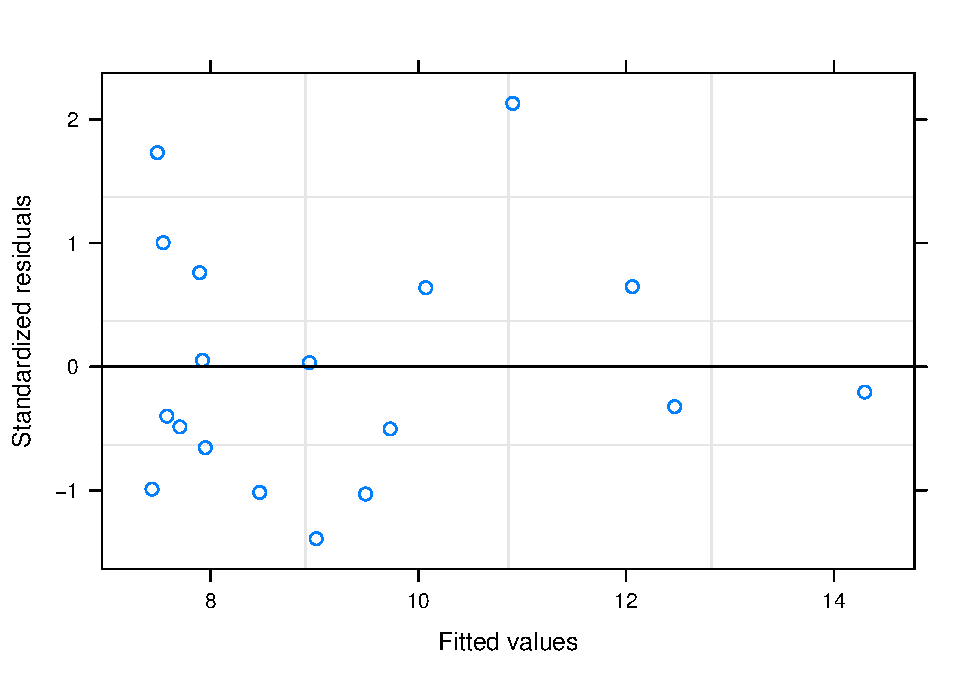
\includegraphics{birdsdataanalysis_files/figure-latex/unnamed-chunk-8-1.pdf}

\begin{Shaded}
\begin{Highlighting}[]
\FunctionTok{qqnorm}\NormalTok{(mod2}\FloatTok{.4}\NormalTok{, }\SpecialCharTok{\textasciitilde{}}\FunctionTok{resid}\NormalTok{(.,}\AttributeTok{type=}\StringTok{"p"}\NormalTok{), }\AttributeTok{abline=}\FunctionTok{c}\NormalTok{(}\DecValTok{0}\NormalTok{,}\DecValTok{1}\NormalTok{)) }\CommentTok{\#check for normality of residuals (should not be completely off the line)}
\end{Highlighting}
\end{Shaded}

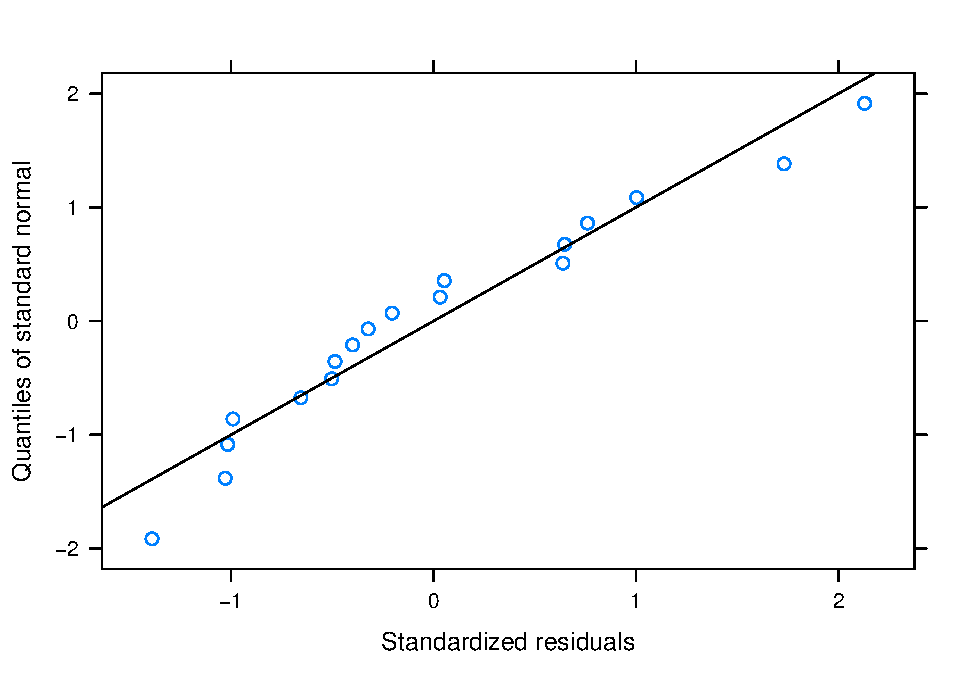
\includegraphics{birdsdataanalysis_files/figure-latex/unnamed-chunk-8-2.pdf}

\begin{Shaded}
\begin{Highlighting}[]
\CommentTok{\#standard deviation, coefficient of variation (sd/mean) to make variation independent from out mean value of dbh\_mean in this case, and check whether is correlated with the other variables and if this is the case we would need to include it in mod2 and check correlation with (vif for the model)  and cor for correlation}

\CommentTok{\#dat$sddbh\_mean \textless{}{-} sd() we can try as alternative}
\FunctionTok{library}\NormalTok{(car)}
\end{Highlighting}
\end{Shaded}

\begin{verbatim}
## Loading required package: carData
\end{verbatim}

\begin{verbatim}
## 
## Attaching package: 'car'
\end{verbatim}

\begin{verbatim}
## The following object is masked from 'package:dplyr':
## 
##     recode
\end{verbatim}

\begin{verbatim}
## The following object is masked from 'package:purrr':
## 
##     some
\end{verbatim}

\begin{Shaded}
\begin{Highlighting}[]
\FunctionTok{vif}\NormalTok{(mod2}\FloatTok{.2}\NormalTok{)}
\end{Highlighting}
\end{Shaded}

\begin{verbatim}
##      category          size  canopy_cover      dbh_mean   temperature 
##      8.297162      4.108259      3.093743      2.163964      1.418070 
## category:size 
##      2.117245
\end{verbatim}

\begin{Shaded}
\begin{Highlighting}[]
\FunctionTok{ggplot}\NormalTok{(dat, }\FunctionTok{aes}\NormalTok{(}\AttributeTok{x =}\NormalTok{ dbh\_mean, }\AttributeTok{y =}\NormalTok{ species\_richness))}\SpecialCharTok{+}
  \FunctionTok{geom\_point}\NormalTok{() }\SpecialCharTok{+}
  \FunctionTok{geom\_smooth}\NormalTok{(}\AttributeTok{method =}\NormalTok{ lm,}\AttributeTok{se =} \ConstantTok{TRUE}\NormalTok{, }\AttributeTok{colour =} \StringTok{\textquotesingle{}green\textquotesingle{}}\NormalTok{, }\AttributeTok{size =} \FloatTok{1.5}\NormalTok{) }\SpecialCharTok{+}\FunctionTok{geom\_text}\NormalTok{(}\AttributeTok{x=}\DecValTok{30}\NormalTok{, }\AttributeTok{y=}\DecValTok{15}\NormalTok{, }\AttributeTok{label=}\StringTok{"p{-}value: 0.0442"}\NormalTok{, }\AttributeTok{size=}\FloatTok{3.5}\NormalTok{) }\SpecialCharTok{+}
  \FunctionTok{geom\_text}\NormalTok{(}\AttributeTok{x=}\DecValTok{30}\NormalTok{,}\AttributeTok{y=}\FloatTok{14.3}\NormalTok{,}\AttributeTok{label=}\FunctionTok{expression}\NormalTok{(}\FunctionTok{paste}\NormalTok{(}\StringTok{"R"}\SpecialCharTok{\^{}}\DecValTok{2}\NormalTok{,}\StringTok{"c: 0.6571"}\NormalTok{)), }\AttributeTok{size=}\FloatTok{3.5}\NormalTok{) }\SpecialCharTok{+}
  \FunctionTok{labs}\NormalTok{(}\AttributeTok{x=}\StringTok{"Mean dbh [cm]"}\NormalTok{, }\AttributeTok{y=}\StringTok{"Observed species richness"}\NormalTok{)}
\end{Highlighting}
\end{Shaded}

\begin{verbatim}
## `geom_smooth()` using formula 'y ~ x'
\end{verbatim}

\begin{verbatim}
## Warning in is.na(x): is.na() aplicado a un objeto que no es (lista o vector) de
## tipo 'expression
\end{verbatim}

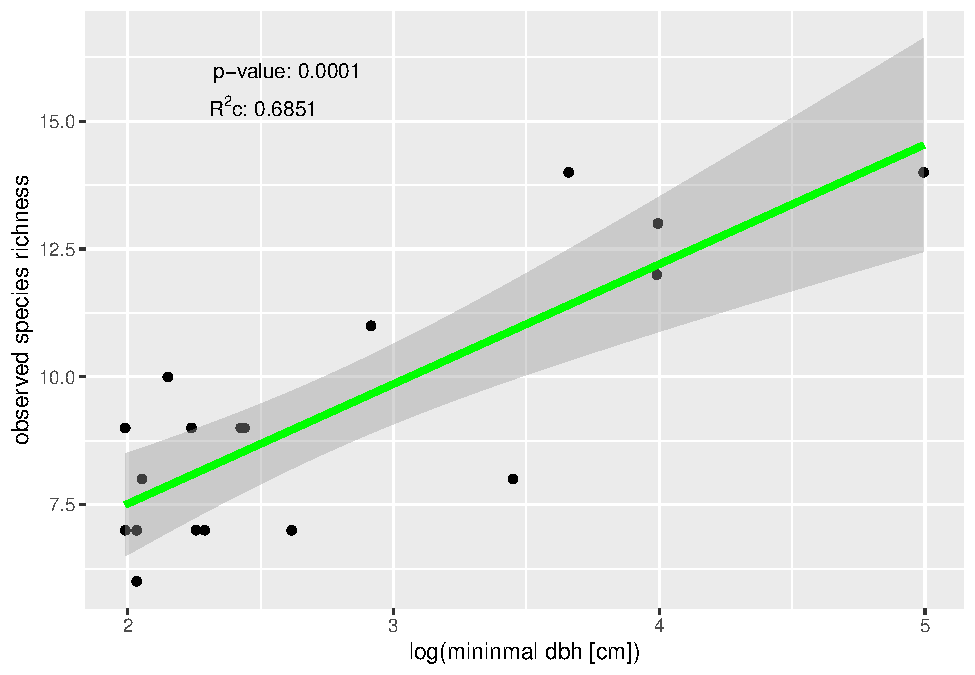
\includegraphics{birdsdataanalysis_files/figure-latex/unnamed-chunk-8-3.pdf}

\#2c Linear Mixed Effect models

\begin{Shaded}
\begin{Highlighting}[]
\DocumentationTok{\#\#\# MIXED EFFECTS MODEL WITH BIRD ABUNDANCE}
\NormalTok{mod3}\FloatTok{.1} \OtherTok{\textless{}{-}} \FunctionTok{lme}\NormalTok{(species\_abund }\SpecialCharTok{\textasciitilde{}}\NormalTok{ category}\SpecialCharTok{*}\NormalTok{size }\SpecialCharTok{+}\NormalTok{ canopy\_cover }\SpecialCharTok{+}\NormalTok{ n\_tree\_spec }\SpecialCharTok{+}\NormalTok{ n\_tree\_ind }\SpecialCharTok{+}\NormalTok{ dbh\_mean }\SpecialCharTok{+}\NormalTok{ n\_microhabitats }\SpecialCharTok{+}\NormalTok{ temperature, }\AttributeTok{random =}\NormalTok{ (}\SpecialCharTok{\textasciitilde{}}\DecValTok{1}\SpecialCharTok{|}\NormalTok{site), }\AttributeTok{data=}\NormalTok{dat, }\AttributeTok{method=}\StringTok{"ML"}\NormalTok{) }\CommentTok{\#initial, full model with all potential predictor variables}
\FunctionTok{summary}\NormalTok{(mod3}\FloatTok{.1}\NormalTok{)}
\end{Highlighting}
\end{Shaded}

\begin{verbatim}
## Linear mixed-effects model fit by maximum likelihood
##   Data: dat 
##        AIC      BIC    logLik
##   108.9707 119.6552 -42.48537
## 
## Random effects:
##  Formula: ~1 | site
##          (Intercept) Residual
## StdDev: 5.560504e-05 2.563465
## 
## Fixed effects:  species_abund ~ category * size + canopy_cover + n_tree_spec +      n_tree_ind + dbh_mean + n_microhabitats + temperature 
##                      Value Std.Error DF    t-value p-value
## (Intercept)       32.60464 11.682637  7  2.7908627  0.0269
## categorypark      -0.52111  6.511040  1 -0.0800347  0.9492
## size              -0.02546  0.026443  1 -0.9629817  0.5120
## canopy_cover      -0.11203  0.061334  7 -1.8265403  0.1105
## n_tree_spec       -0.56638  0.749478  7 -0.7557020  0.4745
## n_tree_ind         0.03783  0.362051  7  0.1044876  0.9197
## dbh_mean           0.09032  0.065994  7  1.3685725  0.2134
## n_microhabitats    0.20644  0.209222  7  0.9867270  0.3566
## temperature       -0.48986  0.387107  1 -1.2654403  0.4257
## categorypark:size  0.01948  0.126341  1  0.1541849  0.9026
##  Correlation: 
##                   (Intr) ctgryp size   cnpy_c n_tr_s n_tr_n dbh_mn n_mcrh
## categorypark      -0.450                                                 
## size              -0.383  0.726                                          
## canopy_cover      -0.622  0.338  0.026                                   
## n_tree_spec       -0.316 -0.403 -0.319  0.131                            
## n_tree_ind        -0.497  0.146 -0.036  0.142  0.430                     
## dbh_mean          -0.151 -0.473 -0.134  0.020  0.173  0.126              
## n_microhabitats   -0.304  0.196  0.084  0.068  0.013 -0.148 -0.412       
## temperature       -0.306  0.294  0.358  0.148 -0.408 -0.528 -0.126  0.504
## categorypark:size -0.004 -0.164 -0.054  0.196 -0.348 -0.514  0.102  0.324
##                   tmprtr
## categorypark            
## size                    
## canopy_cover            
## n_tree_spec             
## n_tree_ind              
## dbh_mean                
## n_microhabitats         
## temperature             
## categorypark:size  0.544
## 
## Standardized Within-Group Residuals:
##        Min         Q1        Med         Q3        Max 
## -1.8191889 -0.7463000 -0.1139194  0.8415455  1.7553733 
## 
## Number of Observations: 18
## Number of Groups: 6
\end{verbatim}

\begin{Shaded}
\begin{Highlighting}[]
\NormalTok{mod3}\FloatTok{.2} \OtherTok{\textless{}{-}} \FunctionTok{stepAIC}\NormalTok{(mod3}\FloatTok{.1}\NormalTok{) }\CommentTok{\#model simplification based on AIC{-}value of the model}
\end{Highlighting}
\end{Shaded}

\begin{verbatim}
## Start:  AIC=108.97
## species_abund ~ category * size + canopy_cover + n_tree_spec + 
##     n_tree_ind + dbh_mean + n_microhabitats + temperature
## 
##                   Df    AIC
## - n_tree_ind       1 107.00
## - category:size    1 107.02
## - n_tree_spec      1 108.21
## <none>               108.97
## - n_microhabitats  1 109.04
## - temperature      1 110.25
## - dbh_mean         1 110.76
## - canopy_cover     1 113.25
## 
## Step:  AIC=107
## species_abund ~ category + size + canopy_cover + n_tree_spec + 
##     dbh_mean + n_microhabitats + temperature + category:size
## 
##                   Df    AIC
## - category:size    1 105.13
## - n_tree_spec      1 106.68
## <none>               107.00
## - n_microhabitats  1 107.17
## - dbh_mean         1 108.77
## - temperature      1 109.06
## - canopy_cover     1 111.46
## 
## Step:  AIC=105.13
## species_abund ~ category + size + canopy_cover + n_tree_spec + 
##     dbh_mean + n_microhabitats + temperature
## 
##                   Df    AIC
## - category         1 103.14
## - n_tree_spec      1 104.70
## - size             1 105.01
## <none>               105.13
## - n_microhabitats  1 105.17
## - dbh_mean         1 106.77
## - temperature      1 108.28
## - canopy_cover     1 110.63
## 
## Step:  AIC=103.14
## species_abund ~ size + canopy_cover + n_tree_spec + dbh_mean + 
##     n_microhabitats + temperature
## 
##                   Df    AIC
## <none>               103.14
## - n_microhabitats  1 103.41
## - n_tree_spec      1 103.54
## - size             1 104.65
## - dbh_mean         1 105.59
## - temperature      1 107.62
## - canopy_cover     1 109.45
\end{verbatim}

\begin{Shaded}
\begin{Highlighting}[]
\FunctionTok{summary}\NormalTok{(mod3}\FloatTok{.2}\NormalTok{) }\CommentTok{\#final model which includes only the most important predictors }
\end{Highlighting}
\end{Shaded}

\begin{verbatim}
## Linear mixed-effects model fit by maximum likelihood
##   Data: dat 
##       AIC      BIC    logLik
##   103.138 111.1513 -42.56899
## 
## Random effects:
##  Formula: ~1 | site
##          (Intercept) Residual
## StdDev: 5.621743e-05 2.575402
## 
## Fixed effects:  species_abund ~ size + canopy_cover + n_tree_spec + dbh_mean +      n_microhabitats + temperature 
##                    Value Std.Error DF   t-value p-value
## (Intercept)     33.72167  6.992167  8  4.822778  0.0013
## size            -0.02344  0.015223  3 -1.539513  0.2213
## canopy_cover    -0.11605  0.045665  8 -2.541310  0.0346
## n_tree_spec     -0.59915  0.477930  8 -1.253643  0.2454
## dbh_mean         0.08409  0.047875  8  1.756428  0.1171
## n_microhabitats  0.19875  0.163453  8  1.215951  0.2587
## temperature     -0.48706  0.222957  3 -2.184566  0.1168
##  Correlation: 
##                 (Intr) size   cnpy_c n_tr_s dbh_mn n_mcrh
## size            -0.257                                   
## canopy_cover    -0.509 -0.348                            
## n_tree_spec     -0.674  0.087  0.449                     
## dbh_mean        -0.387  0.419  0.152 -0.137              
## n_microhabitats -0.291 -0.134 -0.114  0.357 -0.426       
## temperature     -0.641  0.142 -0.038  0.133  0.133  0.377
## 
## Standardized Within-Group Residuals:
##        Min         Q1        Med         Q3        Max 
## -1.8531606 -0.7426492 -0.1486464  0.9509567  1.7573760 
## 
## Number of Observations: 18
## Number of Groups: 6
\end{verbatim}

\begin{Shaded}
\begin{Highlighting}[]
\NormalTok{mod3}\FloatTok{.3} \OtherTok{\textless{}{-}} \FunctionTok{update}\NormalTok{(mod3}\FloatTok{.2}\NormalTok{, }\SpecialCharTok{\textasciitilde{}}\NormalTok{.}\SpecialCharTok{{-}}\NormalTok{n\_tree\_spec)}
\FunctionTok{summary}\NormalTok{(mod3}\FloatTok{.3}\NormalTok{)}
\end{Highlighting}
\end{Shaded}

\begin{verbatim}
## Linear mixed-effects model fit by maximum likelihood
##   Data: dat 
##        AIC      BIC    logLik
##   103.5418 110.6648 -43.77091
## 
## Random effects:
##  Formula: ~1 | site
##         (Intercept) Residual
## StdDev: 6.21064e-05 2.753241
## 
## Fixed effects:  species_abund ~ size + canopy_cover + dbh_mean + n_microhabitats +      temperature 
##                     Value Std.Error DF   t-value p-value
## (Intercept)     27.810467  5.284594  9  5.262555  0.0005
## size            -0.021783  0.015523  3 -1.403242  0.2551
## canopy_cover    -0.090358  0.041769  9 -2.163276  0.0588
## dbh_mean         0.075864  0.048540  9  1.562934  0.1525
## n_microhabitats  0.271843  0.156296  9  1.739285  0.1160
## temperature     -0.449835  0.226172  3 -1.988905  0.1408
##  Correlation: 
##                 (Intr) size   cnpy_c dbh_mn n_mcrh
## size            -0.270                            
## canopy_cover    -0.312 -0.435                     
## dbh_mean        -0.656  0.437  0.241              
## n_microhabitats -0.073 -0.177 -0.329 -0.408       
## temperature     -0.753  0.133 -0.111  0.154  0.356
## 
## Standardized Within-Group Residuals:
##        Min         Q1        Med         Q3        Max 
## -1.8668783 -0.7581271 -0.2371847  0.6284219  1.9514598 
## 
## Number of Observations: 18
## Number of Groups: 6
\end{verbatim}

\begin{Shaded}
\begin{Highlighting}[]
\FunctionTok{anova}\NormalTok{(mod3}\FloatTok{.2}\NormalTok{,mod3}\FloatTok{.3}\NormalTok{)}
\end{Highlighting}
\end{Shaded}

\begin{verbatim}
##        Model df      AIC      BIC    logLik   Test  L.Ratio p-value
## mod3.2     1  9 103.1380 111.1513 -42.56899                        
## mod3.3     2  8 103.5418 110.6648 -43.77091 1 vs 2 2.403841   0.121
\end{verbatim}

\begin{Shaded}
\begin{Highlighting}[]
\NormalTok{mod3}\FloatTok{.4} \OtherTok{\textless{}{-}} \FunctionTok{update}\NormalTok{(mod3}\FloatTok{.3}\NormalTok{, }\SpecialCharTok{\textasciitilde{}}\NormalTok{.}\SpecialCharTok{{-}}\NormalTok{size)}
\FunctionTok{summary}\NormalTok{(mod3}\FloatTok{.4}\NormalTok{)}
\end{Highlighting}
\end{Shaded}

\begin{verbatim}
## Linear mixed-effects model fit by maximum likelihood
##   Data: dat 
##        AIC      BIC    logLik
##   104.2768 110.5094 -45.13838
## 
## Random effects:
##  Formula: ~1 | site
##          (Intercept) Residual
## StdDev: 0.0001004305 2.970556
## 
## Fixed effects:  species_abund ~ canopy_cover + dbh_mean + n_microhabitats + temperature 
##                     Value Std.Error DF   t-value p-value
## (Intercept)     25.808301  5.274581  9  4.892958  0.0009
## canopy_cover    -0.115835  0.038994  9 -2.970616  0.0157
## dbh_mean         0.105631  0.045257  9  2.334014  0.0445
## n_microhabitats  0.233088  0.159467  9  1.461669  0.1779
## temperature     -0.407778  0.232383  4 -1.754769  0.1542
##  Correlation: 
##                 (Intr) cnpy_c dbh_mn n_mcrh
## canopy_cover    -0.495                     
## dbh_mean        -0.621  0.532              
## n_microhabitats -0.127 -0.458 -0.373       
## temperature     -0.751 -0.060  0.107  0.388
## 
## Standardized Within-Group Residuals:
##        Min         Q1        Med         Q3        Max 
## -2.1872017 -0.5423391 -0.1180743  0.6084736  2.0766354 
## 
## Number of Observations: 18
## Number of Groups: 6
\end{verbatim}

\begin{Shaded}
\begin{Highlighting}[]
\FunctionTok{anova}\NormalTok{(mod3}\FloatTok{.3}\NormalTok{,mod3}\FloatTok{.4}\NormalTok{)}
\end{Highlighting}
\end{Shaded}

\begin{verbatim}
##        Model df      AIC      BIC    logLik   Test  L.Ratio p-value
## mod3.3     1  8 103.5418 110.6648 -43.77091                        
## mod3.4     2  7 104.2768 110.5093 -45.13838 1 vs 2 2.734926  0.0982
\end{verbatim}

\begin{Shaded}
\begin{Highlighting}[]
\NormalTok{mod3}\FloatTok{.5} \OtherTok{\textless{}{-}} \FunctionTok{update}\NormalTok{(mod3}\FloatTok{.4}\NormalTok{, }\SpecialCharTok{\textasciitilde{}}\NormalTok{.}\SpecialCharTok{{-}}\NormalTok{n\_microhabitats)}
\FunctionTok{summary}\NormalTok{(mod3}\FloatTok{.5}\NormalTok{)}
\end{Highlighting}
\end{Shaded}

\begin{verbatim}
## Linear mixed-effects model fit by maximum likelihood
##   Data: dat 
##        AIC      BIC   logLik
##   105.0156 110.3578 -46.5078
## 
## Random effects:
##  Formula: ~1 | site
##         (Intercept) Residual
## StdDev: 0.000117092 3.205372
## 
## Fixed effects:  species_abund ~ canopy_cover + dbh_mean + temperature 
##                  Value Std.Error DF   t-value p-value
## (Intercept)  26.787837  5.440044 10  4.924195  0.0006
## canopy_cover -0.089759  0.036053 10 -2.489626  0.0320
## dbh_mean      0.130323  0.043657 10  2.985133  0.0137
## temperature  -0.539737  0.222651  4 -2.424138  0.0724
##  Correlation: 
##              (Intr) cnpy_c dbh_mn
## canopy_cover -0.628              
## dbh_mean     -0.727  0.438       
## temperature  -0.768  0.144  0.295
## 
## Standardized Within-Group Residuals:
##        Min         Q1        Med         Q3        Max 
## -1.6377292 -0.7610096 -0.2370031  0.3374006  2.0931470 
## 
## Number of Observations: 18
## Number of Groups: 6
\end{verbatim}

\begin{Shaded}
\begin{Highlighting}[]
\FunctionTok{anova}\NormalTok{(mod3}\FloatTok{.4}\NormalTok{,mod3}\FloatTok{.5}\NormalTok{)}
\end{Highlighting}
\end{Shaded}

\begin{verbatim}
##        Model df      AIC      BIC    logLik   Test  L.Ratio p-value
## mod3.4     1  7 104.2768 110.5093 -45.13838                        
## mod3.5     2  6 105.0156 110.3578 -46.50780 1 vs 2 2.738846  0.0979
\end{verbatim}

\begin{Shaded}
\begin{Highlighting}[]
\CommentTok{\#mod3.6\textless{}{-} update(mod3.5, \textasciitilde{}.{-}temperature)}
\CommentTok{\#summary(mod3.6)}
\CommentTok{\#anova(mod3.5,mod3.6) \# significant.. 0.0136 so we cannot remove more parameters and final model is 3.5}
\FunctionTok{plot}\NormalTok{(mod3}\FloatTok{.5}\NormalTok{) }\CommentTok{\#check for homogeneity of variances (data points should have similar vertical spread along the x{-}axis)}
\end{Highlighting}
\end{Shaded}

\includegraphics{birdsdataanalysis_files/figure-latex/unnamed-chunk-9-1.pdf}

\begin{Shaded}
\begin{Highlighting}[]
\FunctionTok{qqnorm}\NormalTok{(mod3}\FloatTok{.5}\NormalTok{, }\SpecialCharTok{\textasciitilde{}}\FunctionTok{resid}\NormalTok{(.,}\AttributeTok{type=}\StringTok{"p"}\NormalTok{), }\AttributeTok{abline=}\FunctionTok{c}\NormalTok{(}\DecValTok{0}\NormalTok{,}\DecValTok{1}\NormalTok{)) }\CommentTok{\#check for normality of residuals (should not be completely off the line)}
\end{Highlighting}
\end{Shaded}

\includegraphics{birdsdataanalysis_files/figure-latex/unnamed-chunk-9-2.pdf}

\begin{Shaded}
\begin{Highlighting}[]
\FunctionTok{r.squaredGLMM}\NormalTok{(mod3}\FloatTok{.5}\NormalTok{)}
\end{Highlighting}
\end{Shaded}

\begin{verbatim}
##            R2m       R2c
## [1,] 0.7429521 0.7429521
\end{verbatim}

\#2d Plotting

\begin{Shaded}
\begin{Highlighting}[]
\CommentTok{\# plot model for abundance vs. canopy cover}
\NormalTok{mod\_can}\OtherTok{\textless{}{-}}\FunctionTok{lme}\NormalTok{(species\_abund }\SpecialCharTok{\textasciitilde{}}\NormalTok{ canopy\_cover, }\AttributeTok{random =}\NormalTok{ (}\SpecialCharTok{\textasciitilde{}}\DecValTok{1}\SpecialCharTok{|}\NormalTok{site), }\AttributeTok{data=}\NormalTok{dat, }\AttributeTok{method=}\StringTok{"ML"}\NormalTok{)}
\FunctionTok{r.squaredGLMM}\NormalTok{(mod\_can)}
\end{Highlighting}
\end{Shaded}

\begin{verbatim}
##            R2m       R2c
## [1,] 0.3208035 0.5312365
\end{verbatim}

\begin{Shaded}
\begin{Highlighting}[]
\FunctionTok{ggplot}\NormalTok{(dat, }\FunctionTok{aes}\NormalTok{(}\AttributeTok{x =}\NormalTok{ canopy\_cover, }\AttributeTok{y =}\NormalTok{ species\_abund))}\SpecialCharTok{+}
  \FunctionTok{geom\_point}\NormalTok{() }\SpecialCharTok{+}
  \FunctionTok{geom\_smooth}\NormalTok{(}\AttributeTok{method =}\NormalTok{ lm, }\AttributeTok{se =} \ConstantTok{TRUE}\NormalTok{, }\AttributeTok{colour =} \StringTok{\textquotesingle{}green\textquotesingle{}}\NormalTok{, }\AttributeTok{size =} \FloatTok{1.5}\NormalTok{) }\SpecialCharTok{+}
  \FunctionTok{geom\_text}\NormalTok{(}\AttributeTok{x=}\DecValTok{70}\NormalTok{, }\AttributeTok{y=}\DecValTok{35}\NormalTok{, }\AttributeTok{label=}\StringTok{"p{-}value: 0.0320"}\NormalTok{, }\AttributeTok{size=}\FloatTok{3.5}\NormalTok{) }\SpecialCharTok{+}
  \FunctionTok{geom\_text}\NormalTok{(}\AttributeTok{x=}\DecValTok{70}\NormalTok{,}\AttributeTok{y=}\FloatTok{33.5}\NormalTok{, }\AttributeTok{label=}\FunctionTok{expression}\NormalTok{(}\FunctionTok{paste}\NormalTok{(}\StringTok{"R"}\SpecialCharTok{\^{}}\DecValTok{2}\NormalTok{,}\StringTok{"c: 0.7430"}\NormalTok{)), }\AttributeTok{size=}\FloatTok{3.5}\NormalTok{) }\SpecialCharTok{+}
  \FunctionTok{labs}\NormalTok{(}\AttributeTok{x=}\StringTok{"Canopy cover [\%]"}\NormalTok{, }\AttributeTok{y=}\StringTok{"Species abundance"}\NormalTok{)}
\end{Highlighting}
\end{Shaded}

\begin{verbatim}
## `geom_smooth()` using formula 'y ~ x'
\end{verbatim}

\begin{verbatim}
## Warning in is.na(x): is.na() aplicado a un objeto que no es (lista o vector) de
## tipo 'expression
\end{verbatim}

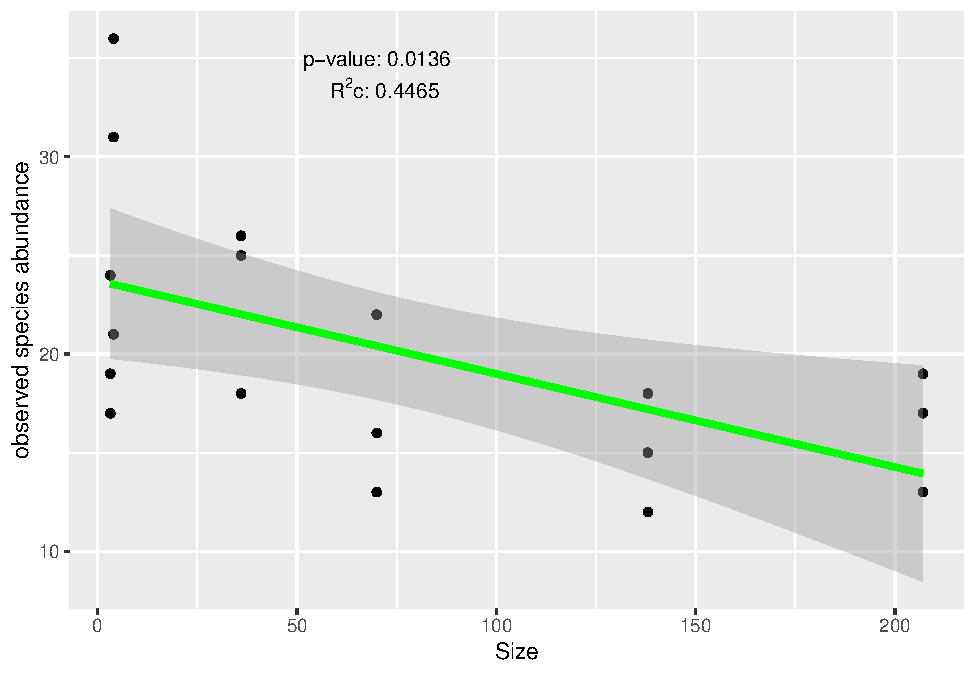
\includegraphics{birdsdataanalysis_files/figure-latex/unnamed-chunk-10-1.pdf}

\begin{Shaded}
\begin{Highlighting}[]
 \CommentTok{\#plot species abundance vs. dbh\_mean}
\NormalTok{mod\_dbh}\OtherTok{\textless{}{-}}\FunctionTok{lme}\NormalTok{(species\_abund }\SpecialCharTok{\textasciitilde{}}\NormalTok{ dbh\_mean, }\AttributeTok{random =}\NormalTok{ (}\SpecialCharTok{\textasciitilde{}}\DecValTok{1}\SpecialCharTok{|}\NormalTok{site), }\AttributeTok{data=}\NormalTok{dat, }\AttributeTok{method=}\StringTok{"ML"}\NormalTok{)}
\FunctionTok{r.squaredGLMM}\NormalTok{(mod\_dbh)}
\end{Highlighting}
\end{Shaded}

\begin{verbatim}
##            R2m       R2c
## [1,] 0.5439872 0.5439872
\end{verbatim}

\begin{Shaded}
\begin{Highlighting}[]
\FunctionTok{ggplot}\NormalTok{(dat, }\FunctionTok{aes}\NormalTok{(}\AttributeTok{x =}\NormalTok{ dbh\_mean, }\AttributeTok{y =}\NormalTok{ species\_abund))}\SpecialCharTok{+}
  \FunctionTok{geom\_point}\NormalTok{() }\SpecialCharTok{+}
  \FunctionTok{geom\_smooth}\NormalTok{(}\AttributeTok{method =}\NormalTok{ lm, }\AttributeTok{se =} \ConstantTok{TRUE}\NormalTok{, }\AttributeTok{colour =} \StringTok{\textquotesingle{}green\textquotesingle{}}\NormalTok{, }\AttributeTok{size =} \FloatTok{1.5}\NormalTok{) }\SpecialCharTok{+}
  \FunctionTok{geom\_text}\NormalTok{(}\AttributeTok{x=}\DecValTok{30}\NormalTok{, }\AttributeTok{y=}\DecValTok{35}\NormalTok{, }\AttributeTok{label=}\StringTok{"p{-}value: 0.0137"}\NormalTok{, }\AttributeTok{size=}\FloatTok{3.5}\NormalTok{) }\SpecialCharTok{+}
  \FunctionTok{geom\_text}\NormalTok{(}\AttributeTok{x=}\DecValTok{30}\NormalTok{,}\AttributeTok{y=}\FloatTok{33.5}\NormalTok{, }\AttributeTok{label=}\FunctionTok{expression}\NormalTok{(}\FunctionTok{paste}\NormalTok{(}\StringTok{"R"}\SpecialCharTok{\^{}}\DecValTok{2}\NormalTok{,}\StringTok{"c: 0.7430"}\NormalTok{)), }\AttributeTok{size=}\FloatTok{3.5}\NormalTok{) }\SpecialCharTok{+}
  \FunctionTok{labs}\NormalTok{(}\AttributeTok{x=}\StringTok{"Mean dbh [cm]"}\NormalTok{, }\AttributeTok{y=}\StringTok{"Species abundance"}\NormalTok{)}
\end{Highlighting}
\end{Shaded}

\begin{verbatim}
## `geom_smooth()` using formula 'y ~ x'
\end{verbatim}

\begin{verbatim}
## Warning in is.na(x): is.na() aplicado a un objeto que no es (lista o vector) de
## tipo 'expression
\end{verbatim}

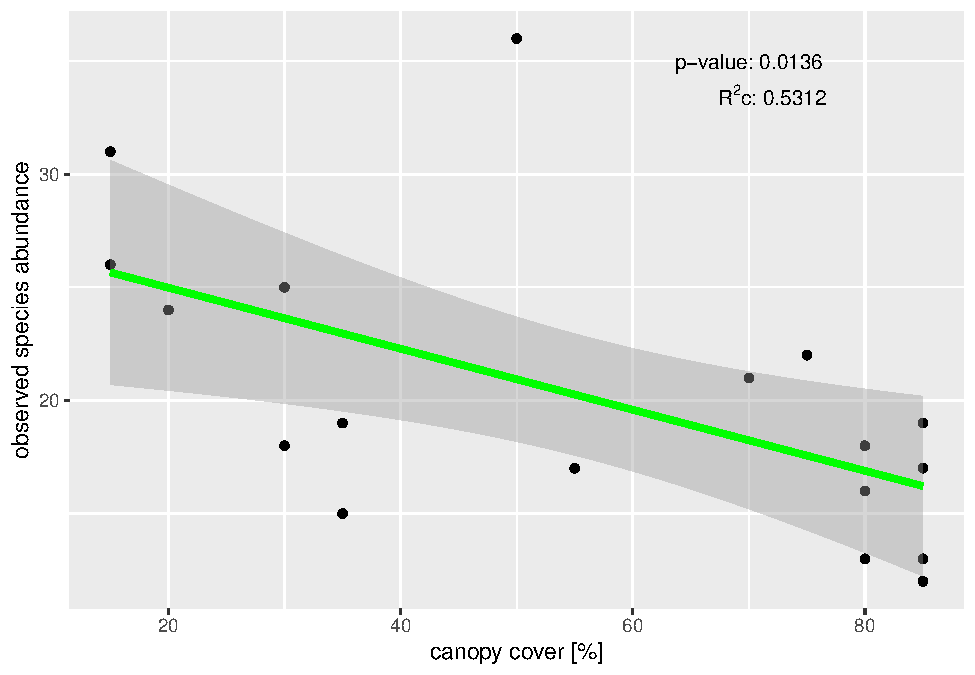
\includegraphics{birdsdataanalysis_files/figure-latex/unnamed-chunk-10-2.pdf}

\begin{Shaded}
\begin{Highlighting}[]
\DocumentationTok{\#\#\# MIXED EFFECTS MODEL WITH RAREFIED RICHNESS}
\NormalTok{mod4 }\OtherTok{\textless{}{-}} \FunctionTok{lme}\NormalTok{(rarefied\_richness }\SpecialCharTok{\textasciitilde{}}\NormalTok{ category}\SpecialCharTok{*}\NormalTok{size }\SpecialCharTok{+}\NormalTok{ canopy\_cover }\SpecialCharTok{+}\NormalTok{ n\_tree\_spec }\SpecialCharTok{+}\NormalTok{ n\_tree\_ind }\SpecialCharTok{+}\NormalTok{ dbh\_mean }\SpecialCharTok{+}\NormalTok{ n\_microhabitats }\SpecialCharTok{+}\NormalTok{ temperature, }\AttributeTok{random =}\NormalTok{ (}\SpecialCharTok{\textasciitilde{}}\DecValTok{1}\SpecialCharTok{|}\NormalTok{site), }\AttributeTok{data=}\NormalTok{dat, }\AttributeTok{method=}\StringTok{"ML"}\NormalTok{) }\CommentTok{\#initial, full model with all potential predictor variables}
\FunctionTok{summary}\NormalTok{(mod4)}
\end{Highlighting}
\end{Shaded}

\begin{verbatim}
## Linear mixed-effects model fit by maximum likelihood
##   Data: dat 
##        AIC      BIC    logLik
##   58.82988 69.51434 -17.41494
## 
## Random effects:
##  Formula: ~1 | site
##          (Intercept)  Residual
## StdDev: 1.945884e-05 0.6367095
## 
## Fixed effects:  rarefied_richness ~ category * size + canopy_cover + n_tree_spec +      n_tree_ind + dbh_mean + n_microhabitats + temperature 
##                       Value Std.Error DF   t-value p-value
## (Intercept)        9.447534 2.9017160  7  3.255844  0.0139
## categorypark      -0.324162 1.6172023  1 -0.200446  0.8741
## size              -0.000690 0.0065679  1 -0.105015  0.9334
## canopy_cover      -0.009385 0.0152341  7 -0.616052  0.5574
## n_tree_spec       -0.239581 0.1861543  7 -1.287001  0.2390
## n_tree_ind        -0.023317 0.0899256  7 -0.259293  0.8029
## dbh_mean           0.015162 0.0163914  7  0.924993  0.3857
## n_microhabitats   -0.019605 0.0519662  7 -0.377270  0.7172
## temperature       -0.038946 0.0961492  1 -0.405056  0.7550
## categorypark:size  0.035628 0.0313803  1  1.135373  0.4597
##  Correlation: 
##                   (Intr) ctgryp size   cnpy_c n_tr_s n_tr_n dbh_mn n_mcrh
## categorypark      -0.450                                                 
## size              -0.383  0.726                                          
## canopy_cover      -0.622  0.338  0.026                                   
## n_tree_spec       -0.316 -0.403 -0.319  0.131                            
## n_tree_ind        -0.497  0.146 -0.036  0.142  0.430                     
## dbh_mean          -0.151 -0.473 -0.134  0.020  0.173  0.126              
## n_microhabitats   -0.304  0.196  0.084  0.068  0.013 -0.148 -0.412       
## temperature       -0.306  0.294  0.358  0.148 -0.408 -0.528 -0.126  0.504
## categorypark:size -0.004 -0.164 -0.054  0.196 -0.348 -0.514  0.102  0.324
##                   tmprtr
## categorypark            
## size                    
## canopy_cover            
## n_tree_spec             
## n_tree_ind              
## dbh_mean                
## n_microhabitats         
## temperature             
## categorypark:size  0.544
## 
## Standardized Within-Group Residuals:
##        Min         Q1        Med         Q3        Max 
## -2.1877031 -0.4447040  0.1760579  0.6684129  1.9167774 
## 
## Number of Observations: 18
## Number of Groups: 6
\end{verbatim}

\begin{Shaded}
\begin{Highlighting}[]
\NormalTok{mod4}\FloatTok{.1} \OtherTok{\textless{}{-}} \FunctionTok{stepAIC}\NormalTok{(mod4) }\CommentTok{\#model simplification based on AIC{-}value of the model}
\end{Highlighting}
\end{Shaded}

\begin{verbatim}
## Start:  AIC=58.83
## rarefied_richness ~ category * size + canopy_cover + n_tree_spec + 
##     n_tree_ind + dbh_mean + n_microhabitats + temperature
## 
##                   Df    AIC
## - n_tree_ind       1 56.981
## - n_microhabitats  1 57.147
## - temperature      1 57.195
## - canopy_cover     1 57.664
## - dbh_mean         1 58.659
## <none>               58.830
## - category:size    1 59.519
## - n_tree_spec      1 60.217
## 
## Step:  AIC=56.98
## rarefied_richness ~ category + size + canopy_cover + n_tree_spec + 
##     dbh_mean + n_microhabitats + temperature + category:size
## 
##                   Df    AIC
## - n_microhabitats  1 55.370
## - canopy_cover     1 55.729
## - temperature      1 55.866
## - dbh_mean         1 56.949
## <none>               56.981
## - category:size    1 57.793
## - n_tree_spec      1 58.393
## 
## Step:  AIC=55.37
## rarefied_richness ~ category + size + canopy_cover + n_tree_spec + 
##     dbh_mean + temperature + category:size
## 
##                 Df    AIC
## - temperature    1 53.893
## - canopy_cover   1 54.017
## - dbh_mean       1 54.952
## <none>             55.370
## - n_tree_spec    1 56.583
## - category:size  1 56.961
## 
## Step:  AIC=53.89
## rarefied_richness ~ category + size + canopy_cover + n_tree_spec + 
##     dbh_mean + category:size
## 
##                 Df    AIC
## - canopy_cover   1 52.295
## - dbh_mean       1 53.774
## <none>             53.893
## - n_tree_spec    1 56.012
## - category:size  1 56.111
## 
## Step:  AIC=52.29
## rarefied_richness ~ category + size + n_tree_spec + dbh_mean + 
##     category:size
## 
##                 Df    AIC
## - dbh_mean       1 52.136
## <none>             52.295
## - n_tree_spec    1 54.053
## - category:size  1 54.782
## 
## Step:  AIC=52.14
## rarefied_richness ~ category + size + n_tree_spec + category:size
## 
##                 Df    AIC
## <none>             52.136
## - category:size  1 53.379
## - n_tree_spec    1 54.605
\end{verbatim}

\begin{Shaded}
\begin{Highlighting}[]
\FunctionTok{summary}\NormalTok{(mod4}\FloatTok{.1}\NormalTok{) }\CommentTok{\#final model which includes only the most important predictors }
\end{Highlighting}
\end{Shaded}

\begin{verbatim}
## Linear mixed-effects model fit by maximum likelihood
##   Data: dat 
##        AIC     BIC   logLik
##   52.13579 58.3684 -19.0679
## 
## Random effects:
##  Formula: ~1 | site
##          (Intercept)  Residual
## StdDev: 2.444494e-05 0.6979478
## 
## Fixed effects:  rarefied_richness ~ category + size + n_tree_spec + category:size 
##                       Value Std.Error DF   t-value p-value
## (Intercept)        7.803922 0.8477467 11  9.205488  0.0000
## categorypark       1.142705 0.9611518  2  1.188892  0.3565
## size               0.001719 0.0049856  2  0.344833  0.7631
## n_tree_spec       -0.267011 0.1296074 11 -2.060150  0.0638
## categorypark:size  0.033118 0.0193783  2  1.709046  0.2296
##  Correlation: 
##                   (Intr) ctgryp size   n_tr_s
## categorypark      -0.391                     
## size              -0.688  0.790              
## n_tree_spec       -0.508 -0.519 -0.190       
## categorypark:size  0.346 -0.278 -0.194 -0.285
## 
## Standardized Within-Group Residuals:
##        Min         Q1        Med         Q3        Max 
## -1.8703378 -0.3878931  0.3183945  0.6351161  1.5813899 
## 
## Number of Observations: 18
## Number of Groups: 6
\end{verbatim}

\begin{Shaded}
\begin{Highlighting}[]
\NormalTok{mod4}\FloatTok{.2}\OtherTok{\textless{}{-}}\FunctionTok{update}\NormalTok{(mod4}\FloatTok{.1}\NormalTok{,}\SpecialCharTok{\textasciitilde{}}\NormalTok{.}\SpecialCharTok{{-}}\NormalTok{n\_tree\_spec)}
\FunctionTok{summary}\NormalTok{(mod4}\FloatTok{.2}\NormalTok{)}
\end{Highlighting}
\end{Shaded}

\begin{verbatim}
## Linear mixed-effects model fit by maximum likelihood
##   Data: dat 
##        AIC      BIC    logLik
##   54.60478 59.94701 -21.30239
## 
## Random effects:
##  Formula: ~1 | site
##         (Intercept) Residual
## StdDev:   0.3534172 0.721987
## 
## Fixed effects:  rarefied_richness ~ category + size + category:size 
##                       Value Std.Error DF   t-value p-value
## (Intercept)        6.917136 0.9544546 12  7.247213  0.0000
## categorypark       0.114911 1.0736401  2  0.107030  0.9245
## size              -0.000234 0.0063966  2 -0.036657  0.9741
## categorypark:size  0.021750 0.0242765  2  0.895932  0.4648
##  Correlation: 
##                   (Intr) ctgryp size  
## categorypark      -0.889              
## size              -0.927  0.824       
## categorypark:size  0.244 -0.520 -0.263
## 
## Standardized Within-Group Residuals:
##        Min         Q1        Med         Q3        Max 
## -1.8890898 -0.2875619  0.1002405  0.7866405  1.5315412 
## 
## Number of Observations: 18
## Number of Groups: 6
\end{verbatim}

\begin{Shaded}
\begin{Highlighting}[]
\FunctionTok{anova}\NormalTok{(mod4}\FloatTok{.1}\NormalTok{,mod4}\FloatTok{.2}\NormalTok{) }\CommentTok{\# significant so final model is 4.1}
\end{Highlighting}
\end{Shaded}

\begin{verbatim}
##        Model df      AIC      BIC    logLik   Test L.Ratio p-value
## mod4.1     1  7 52.13579 58.36840 -19.06790                       
## mod4.2     2  6 54.60478 59.94701 -21.30239 1 vs 2 4.46899  0.0345
\end{verbatim}

\begin{Shaded}
\begin{Highlighting}[]
\CommentTok{\# n\_tree\_spec: p{-}value 0.0638; size: p{-}value 0.7631}
\FunctionTok{plot}\NormalTok{(mod4}\FloatTok{.2}\NormalTok{) }\CommentTok{\#check for homogeneity of variances (data points should have similar vertical spread along the x{-}axis)}
\end{Highlighting}
\end{Shaded}

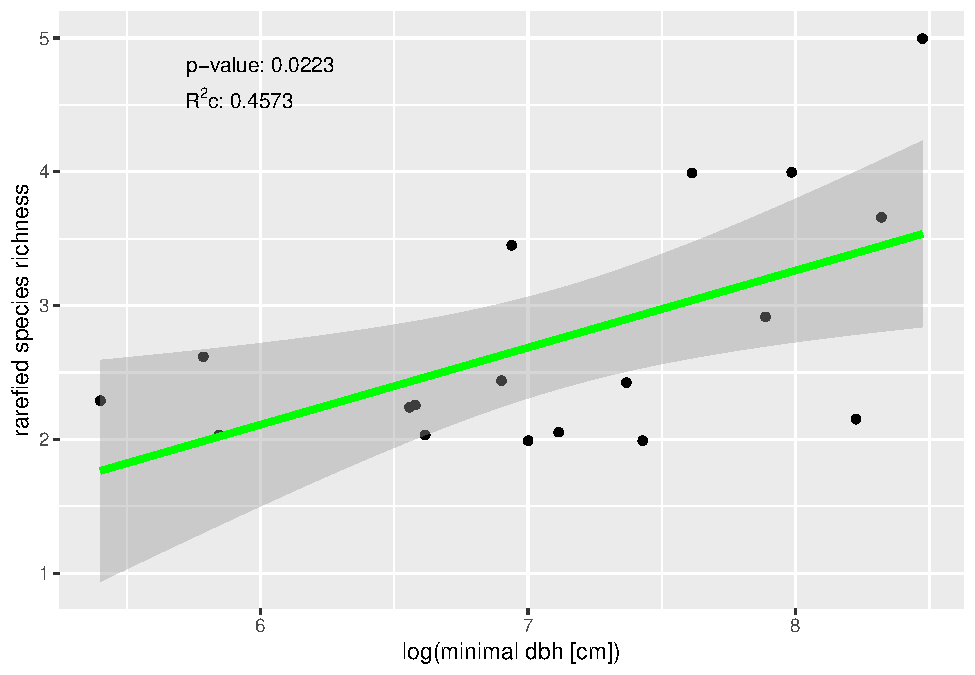
\includegraphics{birdsdataanalysis_files/figure-latex/unnamed-chunk-11-1.pdf}

\begin{Shaded}
\begin{Highlighting}[]
\FunctionTok{qqnorm}\NormalTok{(mod4}\FloatTok{.2}\NormalTok{, }\SpecialCharTok{\textasciitilde{}}\FunctionTok{resid}\NormalTok{(.,}\AttributeTok{type=}\StringTok{"p"}\NormalTok{), }\AttributeTok{abline=}\FunctionTok{c}\NormalTok{(}\DecValTok{0}\NormalTok{,}\DecValTok{1}\NormalTok{)) }\CommentTok{\#check for normality of residuals (should not be completely off the line)}
\end{Highlighting}
\end{Shaded}

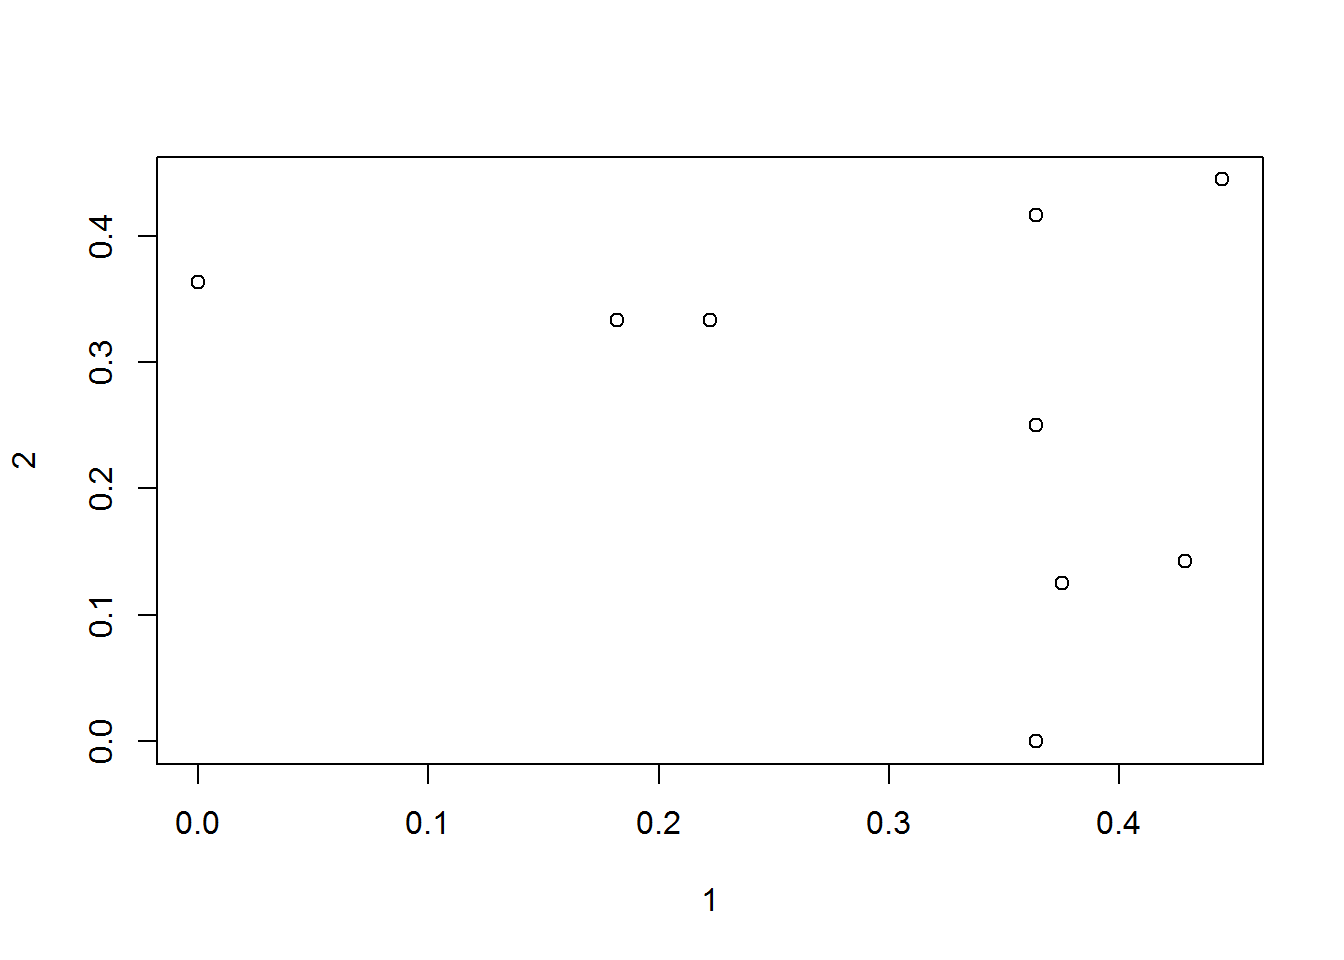
\includegraphics{birdsdataanalysis_files/figure-latex/unnamed-chunk-11-2.pdf}

\begin{Shaded}
\begin{Highlighting}[]
\NormalTok{?qqnorm}
\end{Highlighting}
\end{Shaded}

\begin{verbatim}
## starting httpd help server ... done
\end{verbatim}

\begin{Shaded}
\begin{Highlighting}[]
\NormalTok{?metaMDS}
\NormalTok{?envfit}
\NormalTok{?ordiplot}
\NormalTok{?diversity}
\CommentTok{\#plot(log(dbh\_min)\textasciitilde{}rarefied\_richness, data=dat, ylim=c(0,5))}
\CommentTok{\#mod\textless{}{-}lm(rarefied\_richness \textasciitilde{} log(dbh\_min), data=dat, poly(degree = 2))}
\end{Highlighting}
\end{Shaded}

\#\#2c Ordination with NMDS (to look for differences in species
composition)

\begin{Shaded}
\begin{Highlighting}[]
\NormalTok{nmd1 }\OtherTok{\textless{}{-}} \FunctionTok{metaMDS}\NormalTok{(dat[,}\DecValTok{4}\SpecialCharTok{:}\DecValTok{31}\NormalTok{], }\AttributeTok{distance=}\StringTok{"horn"}\NormalTok{, }\AttributeTok{k=}\DecValTok{2}\NormalTok{) }\CommentTok{\#NMDS analysis based on Morisita{-}Horn{-}Index as a dissimilarity measure}
\end{Highlighting}
\end{Shaded}

\begin{verbatim}
## Run 0 stress 0.1663514 
## Run 1 stress 0.1663514 
## ... New best solution
## ... Procrustes: rmse 1.922127e-05  max resid 4.440788e-05 
## ... Similar to previous best
## Run 2 stress 0.1663514 
## ... New best solution
## ... Procrustes: rmse 7.708673e-05  max resid 0.0002511006 
## ... Similar to previous best
## Run 3 stress 0.174846 
## Run 4 stress 0.1707768 
## Run 5 stress 0.1663514 
## ... New best solution
## ... Procrustes: rmse 6.190013e-05  max resid 0.0002087793 
## ... Similar to previous best
## Run 6 stress 0.1777238 
## Run 7 stress 0.1828469 
## Run 8 stress 0.174846 
## Run 9 stress 0.1663514 
## ... New best solution
## ... Procrustes: rmse 2.648111e-05  max resid 8.81623e-05 
## ... Similar to previous best
## Run 10 stress 0.1663514 
## ... New best solution
## ... Procrustes: rmse 5.553016e-06  max resid 1.643632e-05 
## ... Similar to previous best
## Run 11 stress 0.174846 
## Run 12 stress 0.1663514 
## ... Procrustes: rmse 5.367007e-06  max resid 1.745305e-05 
## ... Similar to previous best
## Run 13 stress 0.1663514 
## ... Procrustes: rmse 5.842874e-06  max resid 1.84341e-05 
## ... Similar to previous best
## Run 14 stress 0.1828469 
## Run 15 stress 0.1828469 
## Run 16 stress 0.1663514 
## ... New best solution
## ... Procrustes: rmse 3.228556e-06  max resid 1.099565e-05 
## ... Similar to previous best
## Run 17 stress 0.1707767 
## Run 18 stress 0.1927819 
## Run 19 stress 0.1927819 
## Run 20 stress 0.1707767 
## *** Solution reached
\end{verbatim}

\begin{Shaded}
\begin{Highlighting}[]
\CommentTok{\# orditkplot(nmd1, display = "species", col = "darkred", fill = NA, border = NA, cex = 0.6)}
\FunctionTok{ordiplot}\NormalTok{(nmd1, }\AttributeTok{choices =} \FunctionTok{c}\NormalTok{(}\DecValTok{1}\NormalTok{, }\DecValTok{2}\NormalTok{), }\AttributeTok{type =} \StringTok{"n"}\NormalTok{) }\CommentTok{\# ylim = c({-}0.75, 0.5), xlim = c({-}1.25, 1.3))}
\FunctionTok{ordilabel}\NormalTok{(nmd1, }\AttributeTok{display =} \StringTok{"species"}\NormalTok{, }\AttributeTok{col =} \StringTok{"darkred"}\NormalTok{, }\AttributeTok{fill =} \ConstantTok{NA}\NormalTok{, }\AttributeTok{border =} \ConstantTok{NA}\NormalTok{, }\AttributeTok{cex =} \FloatTok{0.5}\NormalTok{)}
\FunctionTok{points}\NormalTok{(nmd1, }\AttributeTok{pch=}\FunctionTok{c}\NormalTok{(}\DecValTok{16}\NormalTok{, }\DecValTok{17}\NormalTok{)[}\FunctionTok{as.numeric}\NormalTok{(}\FunctionTok{as.factor}\NormalTok{(dat}\SpecialCharTok{$}\NormalTok{category))], }\AttributeTok{col =} \StringTok{"darkblue"}\NormalTok{) }\CommentTok{\#add sampling points}
\FunctionTok{legend}\NormalTok{(}\StringTok{"topright"}\NormalTok{, }\AttributeTok{pch =} \FunctionTok{c}\NormalTok{(}\DecValTok{16}\NormalTok{, }\DecValTok{17}\NormalTok{), }\FunctionTok{c}\NormalTok{(}\StringTok{"Forest"}\NormalTok{,}\StringTok{"Park"}\NormalTok{), }\AttributeTok{col =} \StringTok{"darkblue"}\NormalTok{, }\AttributeTok{cex =} \FloatTok{0.7}\NormalTok{) }\CommentTok{\#add legend}
\FunctionTok{text}\NormalTok{(}\SpecialCharTok{{-}}\FloatTok{1.4}\NormalTok{, }\SpecialCharTok{{-}}\FloatTok{1.1}\NormalTok{, }\AttributeTok{labels =} \StringTok{"stress = 0.166"}\NormalTok{, }\AttributeTok{cex =} \FloatTok{0.7}\NormalTok{)}

\NormalTok{ef }\OtherTok{\textless{}{-}} \FunctionTok{envfit}\NormalTok{(nmd1, dat[,}\DecValTok{32}\SpecialCharTok{:}\DecValTok{44}\NormalTok{]) }\CommentTok{\#check for correlation of dissimilarity gradients with environmental variables}
\NormalTok{ef }\CommentTok{\#results}
\end{Highlighting}
\end{Shaded}

\begin{verbatim}
## 
## ***VECTORS
## 
##                    NMDS1    NMDS2     r2 Pr(>r)    
## canopy_cover     0.97464 -0.22378 0.5449  0.003 ** 
## n_tree_spec     -0.90908  0.41662 0.5815  0.001 ***
## n_tree_ind       0.98934 -0.14564 0.1254  0.380    
## dbh_min         -0.95999 -0.28003 0.0958  0.492    
## dbh_min5        -0.66028 -0.75102 0.2847  0.073 .  
## dbh_mean        -0.71934 -0.69466 0.3251  0.051 .  
## dbh_max         -0.75683 -0.65361 0.3293  0.047 *  
## dbh_median      -0.64468 -0.76445 0.2933  0.068 .  
## dbh_sd          -0.90588  0.42354 0.5773  0.005 ** 
## n_microhabitats  0.48725 -0.87326 0.2378  0.121    
## latitude         0.66160 -0.74985 0.2294  0.146    
## longitude        0.99958  0.02909 0.4694  0.010 ** 
## size             0.90394  0.42766 0.7395  0.001 ***
## ---
## Signif. codes:  0 '***' 0.001 '**' 0.01 '*' 0.05 '.' 0.1 ' ' 1
## Permutation: free
## Number of permutations: 999
\end{verbatim}

\begin{Shaded}
\begin{Highlighting}[]
\FunctionTok{plot}\NormalTok{(ef, }\AttributeTok{p.max=}\FloatTok{0.05}\NormalTok{, }\AttributeTok{col =} \StringTok{"darkblue"}\NormalTok{, }\AttributeTok{cex =} \FloatTok{0.7}\NormalTok{) }\CommentTok{\#add significant environmental variables to the NMDS plot}
\end{Highlighting}
\end{Shaded}

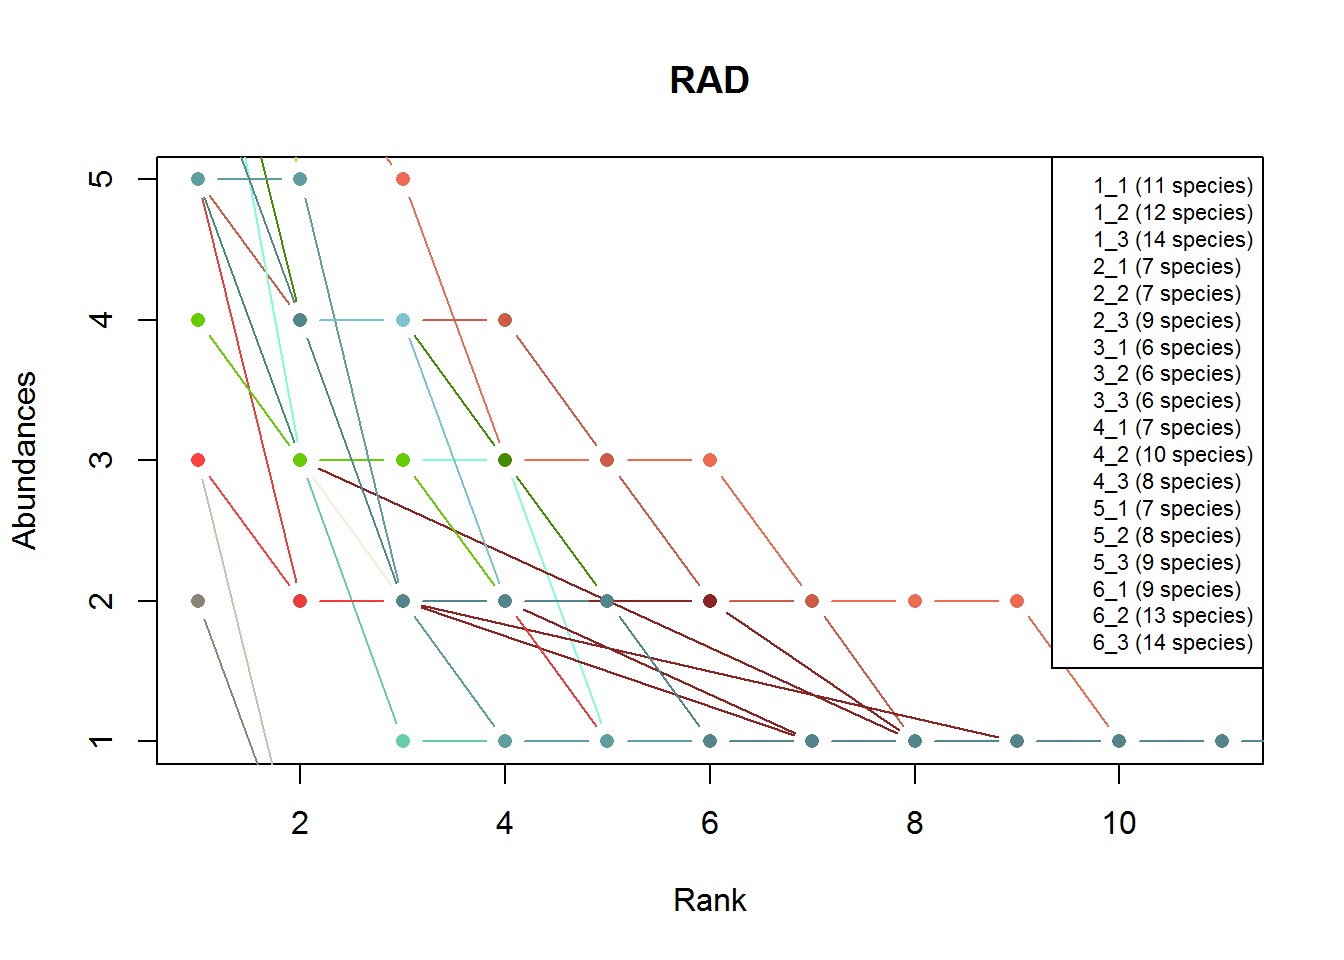
\includegraphics[width=1\linewidth]{birdsdataanalysis_files/figure-latex/unnamed-chunk-12-1}

Now the species accumulation curve is shown.

\begin{Shaded}
\begin{Highlighting}[]
\NormalTok{SAC\_park }\OtherTok{\textless{}{-}} \FunctionTok{specaccum}\NormalTok{(}\FunctionTok{subset}\NormalTok{(dat[,}\DecValTok{4}\SpecialCharTok{:}\DecValTok{31}\NormalTok{], dat}\SpecialCharTok{$}\NormalTok{category }\SpecialCharTok{==} \StringTok{"park"}\NormalTok{))}
\end{Highlighting}
\end{Shaded}

\begin{verbatim}
## Warning in cor(x > 0): the standard deviation is zero
\end{verbatim}

\begin{Shaded}
\begin{Highlighting}[]
\NormalTok{SAC\_fore }\OtherTok{\textless{}{-}} \FunctionTok{specaccum}\NormalTok{(}\FunctionTok{subset}\NormalTok{(dat[,}\DecValTok{4}\SpecialCharTok{:}\DecValTok{31}\NormalTok{], dat}\SpecialCharTok{$}\NormalTok{category }\SpecialCharTok{==} \StringTok{"forest"}\NormalTok{))}
\end{Highlighting}
\end{Shaded}

\begin{verbatim}
## Warning in cor(x > 0): the standard deviation is zero
\end{verbatim}

\begin{Shaded}
\begin{Highlighting}[]
\FunctionTok{plot}\NormalTok{(SAC\_park, }\AttributeTok{xlab =} \StringTok{"Plots"}\NormalTok{, }\AttributeTok{ylab =} \StringTok{"Species richness"}\NormalTok{, }\AttributeTok{main=}\StringTok{"Species accumulation curve"}\NormalTok{)}

\FunctionTok{plot}\NormalTok{(SAC\_fore, }\AttributeTok{xlab =} \StringTok{"Plots"}\NormalTok{, }\AttributeTok{ylab =} \StringTok{"Species richness"}\NormalTok{, }\AttributeTok{main=}\StringTok{"Species accumulation curve"}\NormalTok{, }\AttributeTok{col=}\StringTok{"green"}\NormalTok{, }\AttributeTok{add =}\NormalTok{ T)}
\FunctionTok{legend}\NormalTok{(}\StringTok{"bottomright"}\NormalTok{, }\AttributeTok{legend =} \FunctionTok{c}\NormalTok{(}\StringTok{"Park"}\NormalTok{,}\StringTok{"Forest"}\NormalTok{), }\AttributeTok{col =} \FunctionTok{c}\NormalTok{(}\StringTok{"black"}\NormalTok{,}\StringTok{"green"}\NormalTok{), }\AttributeTok{lwd=}\DecValTok{1}\NormalTok{, }\AttributeTok{bty =} \StringTok{"n"}\NormalTok{)}
\end{Highlighting}
\end{Shaded}

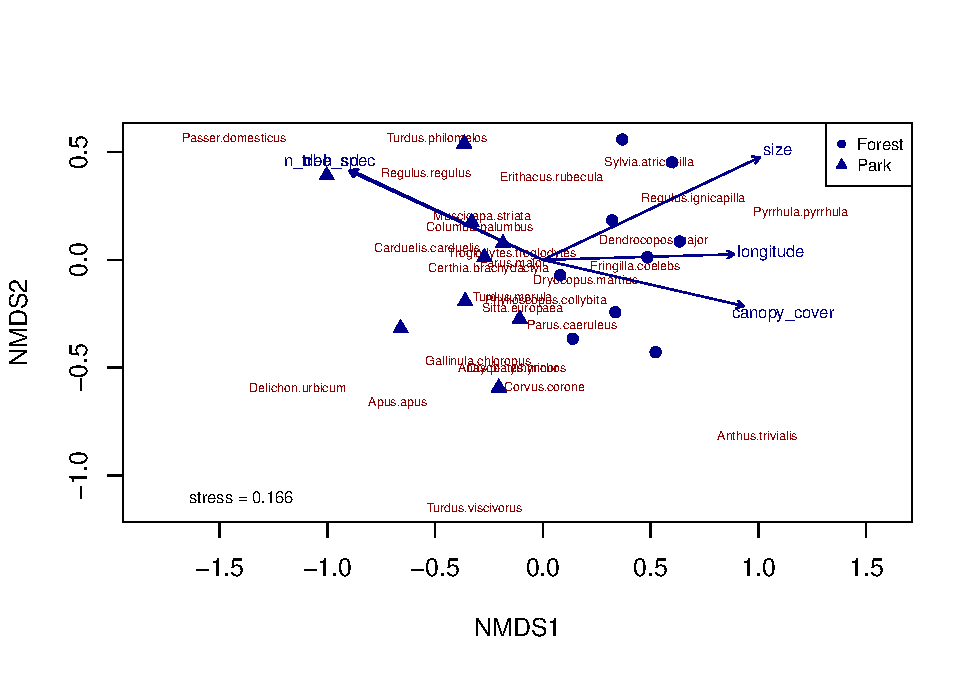
\includegraphics{birdsdataanalysis_files/figure-latex/unnamed-chunk-13-1.pdf}

Analysis of bird's diversity and the variables measured from these two
types of ecosystems.

\begin{Shaded}
\begin{Highlighting}[]
\CommentTok{\# parks \textless{}{-} read.csv("data/parks.csv", sep=";")}
\CommentTok{\# forest \textless{}{-} read.csv("data/forest.csv", sep=";")}
\NormalTok{alpha }\OtherTok{\textless{}{-}} \FunctionTok{specnumber}\NormalTok{(dat[,}\DecValTok{4}\SpecialCharTok{:}\DecValTok{31}\NormalTok{]) }\CommentTok{\# or use the binary site{-}species matrix}
\NormalTok{gamma }\OtherTok{\textless{}{-}} \FunctionTok{ncol}\NormalTok{(dat[,}\FunctionTok{colSums}\NormalTok{(dat[,}\DecValTok{4}\SpecialCharTok{:}\DecValTok{31}\NormalTok{])}\SpecialCharTok{\textgreater{}}\DecValTok{0}\NormalTok{])}

\DocumentationTok{\#\#Lande’s index  (beta) diversity}
\NormalTok{gamma }\SpecialCharTok{{-}} \FunctionTok{mean}\NormalTok{(alpha)}
\end{Highlighting}
\end{Shaded}

\begin{verbatim}
## [1] 38.72222
\end{verbatim}

\begin{Shaded}
\begin{Highlighting}[]
\DocumentationTok{\#\#Whittaker’s index}

\CommentTok{\#gamma/mean(alpha)}


\CommentTok{\#For parks}

\NormalTok{alphap }\OtherTok{\textless{}{-}} \FunctionTok{specnumber}\NormalTok{(park[,}\DecValTok{4}\SpecialCharTok{:}\DecValTok{31}\NormalTok{])}

\NormalTok{gammap }\OtherTok{\textless{}{-}} \FunctionTok{ncol}\NormalTok{(park[,}\FunctionTok{colSums}\NormalTok{(park[,}\DecValTok{4}\SpecialCharTok{:}\DecValTok{31}\NormalTok{]) }\SpecialCharTok{\textgreater{}} \DecValTok{0}\NormalTok{])}

\DocumentationTok{\#\#Lande’s index }
\NormalTok{gammap }\SpecialCharTok{{-}} \FunctionTok{mean}\NormalTok{(alphap)}
\end{Highlighting}
\end{Shaded}

\begin{verbatim}
## [1] 31.22222
\end{verbatim}

\begin{Shaded}
\begin{Highlighting}[]
\DocumentationTok{\#\#Whittaker’s index}

\CommentTok{\#gammap/mean(alphap)}

\CommentTok{\#For forest}
\NormalTok{alphaf }\OtherTok{\textless{}{-}} \FunctionTok{specnumber}\NormalTok{(forest[,}\DecValTok{4}\SpecialCharTok{:}\DecValTok{31}\NormalTok{])}

\NormalTok{gammaf }\OtherTok{\textless{}{-}} \FunctionTok{ncol}\NormalTok{(park[,}\FunctionTok{colSums}\NormalTok{(park[,}\DecValTok{4}\SpecialCharTok{:}\DecValTok{31}\NormalTok{]) }\SpecialCharTok{\textgreater{}} \DecValTok{0}\NormalTok{])}

\DocumentationTok{\#\#Lande’s index }
\NormalTok{gammaf }\SpecialCharTok{{-}} \FunctionTok{mean}\NormalTok{(alphaf)}
\end{Highlighting}
\end{Shaded}

\begin{verbatim}
## [1] 34.22222
\end{verbatim}

\begin{Shaded}
\begin{Highlighting}[]
\DocumentationTok{\#\#Whittaker’s index}

\CommentTok{\#gammaf/mean(alphaf)}
\end{Highlighting}
\end{Shaded}

The number of shared and unique species for a given for the two plots
combine and separated.

\begin{Shaded}
\begin{Highlighting}[]
\NormalTok{beta\_virt }\OtherTok{\textless{}{-}} \FunctionTok{betadiver}\NormalTok{(dat[,}\DecValTok{4}\SpecialCharTok{:}\DecValTok{31}\NormalTok{], }\AttributeTok{method =} \ConstantTok{NA}\NormalTok{)}
\CommentTok{\# a}
\NormalTok{beta\_virt}\SpecialCharTok{$}\NormalTok{a}
\end{Highlighting}
\end{Shaded}

\begin{verbatim}
##     1  2  3  4  5  6  7  8  9 10 11 12 13 14 15 16 17
## 2   7                                                
## 3   7  9                                             
## 4   4  5  4                                          
## 5   6  6  6  5                                       
## 6   5  5  7  4  5                                    
## 7   4  5  5  3  3  2                                 
## 8   5  6  7  4  4  6  4                              
## 9   5  6  6  3  4  4  4  6                           
## 10  4  5  5  4  5  5  2  5  4                        
## 11  7  8  8  6  7  6  5  7  6  7                     
## 12  5  6  7  4  6  6  3  6  5  6  7                  
## 13  4  6  7  3  4  4  3  5  5  4  5  5               
## 14  5  7  7  4  4  5  4  7  6  5  7  5  6            
## 15  5  5  6  3  4  4  2  4  4  4  5  5  5  5         
## 16  7  6  8  4  6  7  3  5  4  4  6  6  4  4  4      
## 17  9  8  9  5  6  7  5  7  7  6  9  6  5  7  6  8   
## 18  7  7  8  6  5  7  4  7  6  5  7  6  5  6  6  8 11
\end{verbatim}

\begin{Shaded}
\begin{Highlighting}[]
\NormalTok{beta\_virt}\SpecialCharTok{$}\NormalTok{b}
\end{Highlighting}
\end{Shaded}

\begin{verbatim}
##     1  2  3  4  5  6  7  8  9 10 11 12 13 14 15 16 17
## 2   5                                                
## 3   7  5                                             
## 4   3  2  3                                          
## 5   1  1  1  2                                       
## 6   4  4  2  5  4                                    
## 7   2  1  1  3  3  4                                 
## 8   4  3  2  5  5  3  5                              
## 9   2  1  1  4  3  3  3  1                           
## 10  3  2  2  3  2  2  5  2  3                        
## 11  3  2  2  4  3  4  5  3  4  3                     
## 12  3  2  1  4  2  2  5  2  3  2  1                  
## 13  3  1  0  4  3  3  4  2  2  3  2  2               
## 14  3  1  1  4  4  3  4  1  2  3  1  3  2            
## 15  4  4  3  6  5  5  7  5  5  5  4  4  4  4         
## 16  2  3  1  5  3  2  6  4  5  5  3  3  5  5  5      
## 17  4  5  4  8  7  6  8  6  6  7  4  7  8  6  7  5   
## 18  7  7  6  8  9  7 10  7  8  9  7  8  9  8  8  6  3
\end{verbatim}

\begin{Shaded}
\begin{Highlighting}[]
\NormalTok{beta\_virt}\SpecialCharTok{$}\NormalTok{c}
\end{Highlighting}
\end{Shaded}

\begin{verbatim}
##     1  2  3  4  5  6  7  8  9 10 11 12 13 14 15 16 17
## 2   4                                                
## 3   4  3                                             
## 4   7  7 10                                          
## 5   5  6  8  2                                       
## 6   6  7  7  3  2                                    
## 7   7  7  9  4  4  7                                 
## 8   6  6  7  3  3  3  2                              
## 9   6  6  8  4  3  5  2  3                           
## 10  7  7  9  3  2  4  4  4  3                        
## 11  4  4  6  1  0  3  1  2  1  0                     
## 12  6  6  7  3  1  3  3  3  2  1  3                  
## 13  7  6  7  4  3  5  3  4  2  3  5  3               
## 14  6  5  7  3  3  4  2  2  1  2  3  3  1            
## 15  6  7  8  4  3  5  4  5  3  3  5  3  2  3         
## 16  4  6  6  3  1  2  3  4  3  3  4  2  3  4  5      
## 17  2  4  5  2  1  2  1  2  0  1  1  2  2  1  3  1   
## 18  4  5  6  1  2  2  2  2  1  2  3  2  2  2  3  1  2
\end{verbatim}

\begin{Shaded}
\begin{Highlighting}[]
\FunctionTok{plot}\NormalTok{(}\FunctionTok{betadiver}\NormalTok{(dat[,}\DecValTok{4}\SpecialCharTok{:}\DecValTok{31}\NormalTok{], }\AttributeTok{method=}\ConstantTok{NA}\NormalTok{), }\AttributeTok{pch =} \DecValTok{16}\NormalTok{, }\AttributeTok{cex =} \DecValTok{2}\NormalTok{,)}
\FunctionTok{legend}\NormalTok{(}\StringTok{"topleft"}\NormalTok{, }\AttributeTok{legend =} \StringTok{"Virtual matrix"}\NormalTok{, }\AttributeTok{bty =} \StringTok{"n"}\NormalTok{)}
\end{Highlighting}
\end{Shaded}

\includegraphics{birdsdataanalysis_files/figure-latex/unnamed-chunk-15-1.pdf}

\begin{Shaded}
\begin{Highlighting}[]
\NormalTok{beta\_virtp }\OtherTok{\textless{}{-}} \FunctionTok{betadiver}\NormalTok{(park, }\AttributeTok{method =} \ConstantTok{NA}\NormalTok{)}
\end{Highlighting}
\end{Shaded}

\begin{verbatim}
## Warning in Ops.factor(left, right): '>' not meaningful for factors

## Warning in Ops.factor(left, right): '>' not meaningful for factors
\end{verbatim}

\begin{Shaded}
\begin{Highlighting}[]
\CommentTok{\# a}
\NormalTok{beta\_virtp}\SpecialCharTok{$}\NormalTok{a}
\end{Highlighting}
\end{Shaded}

\begin{verbatim}
##     1  2  3 13 14 15 16 17
## 2  NA                     
## 3  NA NA                  
## 13 NA NA NA               
## 14 NA NA NA NA            
## 15 NA NA NA NA NA         
## 16 NA NA NA NA NA NA      
## 17 NA NA NA NA NA NA NA   
## 18 NA NA NA NA NA NA NA NA
\end{verbatim}

\begin{Shaded}
\begin{Highlighting}[]
\NormalTok{beta\_virtp}\SpecialCharTok{$}\NormalTok{b}
\end{Highlighting}
\end{Shaded}

\begin{verbatim}
##     1  2  3 13 14 15 16 17
## 2  NA                     
## 3  NA NA                  
## 13 NA NA NA               
## 14 NA NA NA NA            
## 15 NA NA NA NA NA         
## 16 NA NA NA NA NA NA      
## 17 NA NA NA NA NA NA NA   
## 18 NA NA NA NA NA NA NA NA
\end{verbatim}

\begin{Shaded}
\begin{Highlighting}[]
\NormalTok{beta\_virtp}\SpecialCharTok{$}\NormalTok{c}
\end{Highlighting}
\end{Shaded}

\begin{verbatim}
##     1  2  3 13 14 15 16 17
## 2  NA                     
## 3  NA NA                  
## 13 NA NA NA               
## 14 NA NA NA NA            
## 15 NA NA NA NA NA         
## 16 NA NA NA NA NA NA      
## 17 NA NA NA NA NA NA NA   
## 18 NA NA NA NA NA NA NA NA
\end{verbatim}

\begin{Shaded}
\begin{Highlighting}[]
\FunctionTok{plot}\NormalTok{(}\FunctionTok{betadiver}\NormalTok{(park, }\AttributeTok{method=}\ConstantTok{NA}\NormalTok{), }\AttributeTok{pch =} \DecValTok{16}\NormalTok{, }\AttributeTok{cex =} \DecValTok{2}\NormalTok{,)}
\end{Highlighting}
\end{Shaded}

\begin{verbatim}
## Warning in Ops.factor(left, right): '>' not meaningful for factors

## Warning in Ops.factor(left, right): '>' not meaningful for factors
\end{verbatim}

\begin{Shaded}
\begin{Highlighting}[]
\FunctionTok{legend}\NormalTok{(}\StringTok{"topleft"}\NormalTok{, }\AttributeTok{legend =} \StringTok{"Virtual matrix"}\NormalTok{, }\AttributeTok{bty =} \StringTok{"n"}\NormalTok{)}
\end{Highlighting}
\end{Shaded}

\includegraphics{birdsdataanalysis_files/figure-latex/unnamed-chunk-15-2.pdf}

\begin{Shaded}
\begin{Highlighting}[]
\CommentTok{\#vennd iagram \textless{}{-} as alternative to show the overlap of shared species    }
\end{Highlighting}
\end{Shaded}

We can see how nice heterogeneity is present between the two ecosystems

Now the similarity between plots by Sorensen, Simpson and Jaccard

\begin{Shaded}
\begin{Highlighting}[]
\CommentTok{\#Sorensen similarity}
\NormalTok{sorparks }\OtherTok{\textless{}{-}}  \FunctionTok{betadiver}\NormalTok{(park[,}\DecValTok{4}\SpecialCharTok{:}\DecValTok{31}\NormalTok{], }\AttributeTok{method =} \StringTok{"sor"}\NormalTok{)}
\NormalTok{sorensen }\OtherTok{\textless{}{-}}  \FunctionTok{as.matrix}\NormalTok{(sorparks)[,]}
\FunctionTok{plot}\NormalTok{(sorensen)}
\end{Highlighting}
\end{Shaded}

\includegraphics{birdsdataanalysis_files/figure-latex/unnamed-chunk-16-1.pdf}

\begin{Shaded}
\begin{Highlighting}[]
\CommentTok{\#Simpson similarity}
\NormalTok{simpark}\OtherTok{\textless{}{-}} \FunctionTok{betadiver}\NormalTok{(park[,}\DecValTok{4}\SpecialCharTok{:}\DecValTok{31}\NormalTok{], }\AttributeTok{method =} \StringTok{"sim"}\NormalTok{)}
\NormalTok{simpsonpark }\OtherTok{\textless{}{-}} \FunctionTok{as.matrix}\NormalTok{(simpark)[,]}
\FunctionTok{plot}\NormalTok{(simpsonpark)}
\end{Highlighting}
\end{Shaded}

\includegraphics{birdsdataanalysis_files/figure-latex/unnamed-chunk-16-2.pdf}

\begin{Shaded}
\begin{Highlighting}[]
\CommentTok{\# Jaccard similarity}
\NormalTok{jparks }\OtherTok{\textless{}{-}} \FunctionTok{betadiver}\NormalTok{(park[,}\DecValTok{4}\SpecialCharTok{:}\DecValTok{31}\NormalTok{], }\AttributeTok{method =} \StringTok{"j"}\NormalTok{)}
\FunctionTok{plot}\NormalTok{(}\FunctionTok{as.matrix}\NormalTok{(jparks)[,])}
\end{Highlighting}
\end{Shaded}

\includegraphics{birdsdataanalysis_files/figure-latex/unnamed-chunk-16-3.pdf}

\begin{Shaded}
\begin{Highlighting}[]
\CommentTok{\#Sorensen similarity}
\NormalTok{sorforest }\OtherTok{\textless{}{-}}  \FunctionTok{betadiver}\NormalTok{(forest[,}\DecValTok{4}\SpecialCharTok{:}\DecValTok{31}\NormalTok{], }\AttributeTok{method =} \StringTok{"sor"}\NormalTok{)}
\NormalTok{sorensenforest }\OtherTok{\textless{}{-}}  \FunctionTok{as.matrix}\NormalTok{(sorforest)[,]}
\FunctionTok{plot}\NormalTok{(sorensen)}
\end{Highlighting}
\end{Shaded}

\includegraphics{birdsdataanalysis_files/figure-latex/unnamed-chunk-16-4.pdf}

\begin{Shaded}
\begin{Highlighting}[]
\CommentTok{\#Simpson similarity}
\NormalTok{simf }\OtherTok{\textless{}{-}} \FunctionTok{betadiver}\NormalTok{(forest[,}\DecValTok{4}\SpecialCharTok{:}\DecValTok{31}\NormalTok{], }\AttributeTok{method =} \StringTok{"sim"}\NormalTok{)}
\NormalTok{simpson }\OtherTok{\textless{}{-}} \FunctionTok{as.matrix}\NormalTok{(simf)[,]}
\FunctionTok{plot}\NormalTok{(simpson)}
\end{Highlighting}
\end{Shaded}

\includegraphics{birdsdataanalysis_files/figure-latex/unnamed-chunk-16-5.pdf}

\begin{Shaded}
\begin{Highlighting}[]
\CommentTok{\# Jaccard similarity}

\NormalTok{jforest }\OtherTok{\textless{}{-}} \FunctionTok{betadiver}\NormalTok{(forest[,}\DecValTok{4}\SpecialCharTok{:}\DecValTok{31}\NormalTok{], }\AttributeTok{method =} \StringTok{"j"}\NormalTok{)}
\FunctionTok{as.matrix}\NormalTok{(jforest)[,]}
\end{Highlighting}
\end{Shaded}

\begin{verbatim}
##            4         5         6         7         8         9        10
## 4  0.0000000 0.5555556 0.3333333 0.3000000 0.3333333 0.2727273 0.4000000
## 5  0.5555556 0.0000000 0.4545455 0.3000000 0.3333333 0.4000000 0.5555556
## 6  0.3333333 0.4545455 0.0000000 0.1538462 0.5000000 0.3333333 0.4545455
## 7  0.3000000 0.3000000 0.1538462 0.0000000 0.3636364 0.4444444 0.1818182
## 8  0.3333333 0.3333333 0.5000000 0.3636364 0.0000000 0.6000000 0.4545455
## 9  0.2727273 0.4000000 0.3333333 0.4444444 0.6000000 0.0000000 0.4000000
## 10 0.4000000 0.5555556 0.4545455 0.1818182 0.4545455 0.4000000 0.0000000
## 11 0.5454545 0.7000000 0.4615385 0.4545455 0.5833333 0.5454545 0.7000000
## 12 0.3636364 0.6666667 0.5454545 0.2727273 0.5454545 0.5000000 0.6666667
##           11        12
## 4  0.5454545 0.3636364
## 5  0.7000000 0.6666667
## 6  0.4615385 0.5454545
## 7  0.4545455 0.2727273
## 8  0.5833333 0.5454545
## 9  0.5454545 0.5000000
## 10 0.7000000 0.6666667
## 11 0.0000000 0.6363636
## 12 0.6363636 0.0000000
\end{verbatim}

\begin{Shaded}
\begin{Highlighting}[]
\FunctionTok{plot}\NormalTok{(}\FunctionTok{as.matrix}\NormalTok{(jforest)[,])}
\end{Highlighting}
\end{Shaded}

\includegraphics{birdsdataanalysis_files/figure-latex/unnamed-chunk-16-6.pdf}

\begin{Shaded}
\begin{Highlighting}[]
\CommentTok{\#calculate mean of these similarities indices and compare between sites}
\end{Highlighting}
\end{Shaded}

RANK abundance curve \textless- takes abundant species per site and plot
it against relative species abundance rank

\begin{Shaded}
\begin{Highlighting}[]
\CommentTok{\# Klosterpark}
\NormalTok{plot1\_1 }\OtherTok{\textless{}{-}} \FunctionTok{data.frame}\NormalTok{(}\AttributeTok{sp =} \FunctionTok{colnames}\NormalTok{(dat[,}\DecValTok{4}\SpecialCharTok{:}\DecValTok{31}\NormalTok{]), }\AttributeTok{ab =} \FunctionTok{as.numeric}\NormalTok{(dat[}\DecValTok{1}\NormalTok{,}\DecValTok{4}\SpecialCharTok{:}\DecValTok{31}\NormalTok{]))}
\NormalTok{plot1\_2 }\OtherTok{\textless{}{-}} \FunctionTok{data.frame}\NormalTok{(}\AttributeTok{sp =} \FunctionTok{colnames}\NormalTok{(dat[,}\DecValTok{4}\SpecialCharTok{:}\DecValTok{31}\NormalTok{]), }\AttributeTok{ab =} \FunctionTok{as.numeric}\NormalTok{(dat[}\DecValTok{2}\NormalTok{,}\DecValTok{4}\SpecialCharTok{:}\DecValTok{31}\NormalTok{]))}
\NormalTok{plot1\_3 }\OtherTok{\textless{}{-}} \FunctionTok{data.frame}\NormalTok{(}\AttributeTok{sp =} \FunctionTok{colnames}\NormalTok{(dat[,}\DecValTok{4}\SpecialCharTok{:}\DecValTok{31}\NormalTok{]), }\AttributeTok{ab =} \FunctionTok{as.numeric}\NormalTok{(dat[}\DecValTok{3}\NormalTok{,}\DecValTok{4}\SpecialCharTok{:}\DecValTok{31}\NormalTok{]))}

\NormalTok{plot1\_12 }\OtherTok{\textless{}{-}} \FunctionTok{merge}\NormalTok{(plot1\_1, plot1\_2, }\AttributeTok{by =} \StringTok{"sp"}\NormalTok{)}
\NormalTok{plot1 }\OtherTok{\textless{}{-}} \FunctionTok{merge}\NormalTok{(plot1\_12, plot1\_3, }\AttributeTok{by =} \StringTok{"sp"}\NormalTok{)}
\NormalTok{plot1}\SpecialCharTok{$}\NormalTok{abun }\OtherTok{\textless{}{-}}\NormalTok{ plot1}\SpecialCharTok{$}\NormalTok{ab.x }\SpecialCharTok{+}\NormalTok{ plot1}\SpecialCharTok{$}\NormalTok{ab.y }\SpecialCharTok{+}\NormalTok{ plot1}\SpecialCharTok{$}\NormalTok{ab}
\NormalTok{plot1 }\OtherTok{\textless{}{-}}\NormalTok{ plot1[}\FunctionTok{which}\NormalTok{(plot1}\SpecialCharTok{$}\NormalTok{abun}\SpecialCharTok{!=}\DecValTok{0}\NormalTok{),]}
\FunctionTok{dim}\NormalTok{(plot1)}
\end{Highlighting}
\end{Shaded}

\begin{verbatim}
## [1] 20  5
\end{verbatim}

\begin{Shaded}
\begin{Highlighting}[]
\NormalTok{plot1}\SpecialCharTok{$}\NormalTok{relabun }\OtherTok{\textless{}{-}}\NormalTok{ plot1}\SpecialCharTok{$}\NormalTok{abun }\SpecialCharTok{*} \DecValTok{100} \SpecialCharTok{/} \FunctionTok{sum}\NormalTok{(plot1}\SpecialCharTok{$}\NormalTok{abun)}
\NormalTok{plot1}\SpecialCharTok{$}\NormalTok{rank }\OtherTok{\textless{}{-}} \FunctionTok{rank}\NormalTok{(}\SpecialCharTok{{-}}\NormalTok{plot1}\SpecialCharTok{$}\NormalTok{relabun, }\AttributeTok{ties.method =} \StringTok{"random"}\NormalTok{)}
\NormalTok{plot1 }\OtherTok{\textless{}{-}}\NormalTok{ plot1[}\FunctionTok{order}\NormalTok{(plot1}\SpecialCharTok{$}\NormalTok{rank),]}

\CommentTok{\# City Forest}
\NormalTok{plot2\_1 }\OtherTok{\textless{}{-}} \FunctionTok{data.frame}\NormalTok{(}\AttributeTok{sp =} \FunctionTok{colnames}\NormalTok{(dat[,}\DecValTok{4}\SpecialCharTok{:}\DecValTok{31}\NormalTok{]), }\AttributeTok{ab =} \FunctionTok{as.numeric}\NormalTok{(dat[}\DecValTok{4}\NormalTok{,}\DecValTok{4}\SpecialCharTok{:}\DecValTok{31}\NormalTok{]))}
\NormalTok{plot2\_2 }\OtherTok{\textless{}{-}} \FunctionTok{data.frame}\NormalTok{(}\AttributeTok{sp =} \FunctionTok{colnames}\NormalTok{(dat[,}\DecValTok{4}\SpecialCharTok{:}\DecValTok{31}\NormalTok{]), }\AttributeTok{ab =} \FunctionTok{as.numeric}\NormalTok{(dat[}\DecValTok{5}\NormalTok{,}\DecValTok{4}\SpecialCharTok{:}\DecValTok{31}\NormalTok{]))}
\NormalTok{plot2\_3 }\OtherTok{\textless{}{-}} \FunctionTok{data.frame}\NormalTok{(}\AttributeTok{sp =} \FunctionTok{colnames}\NormalTok{(dat[,}\DecValTok{4}\SpecialCharTok{:}\DecValTok{31}\NormalTok{]), }\AttributeTok{ab =} \FunctionTok{as.numeric}\NormalTok{(dat[}\DecValTok{6}\NormalTok{,}\DecValTok{4}\SpecialCharTok{:}\DecValTok{31}\NormalTok{]))}

\NormalTok{plot2\_12 }\OtherTok{\textless{}{-}} \FunctionTok{merge}\NormalTok{(plot2\_1, plot2\_2, }\AttributeTok{by =} \StringTok{"sp"}\NormalTok{)}
\NormalTok{plot2 }\OtherTok{\textless{}{-}} \FunctionTok{merge}\NormalTok{(plot2\_12, plot2\_3, }\AttributeTok{by =} \StringTok{"sp"}\NormalTok{)}
\NormalTok{plot2}\SpecialCharTok{$}\NormalTok{abun }\OtherTok{\textless{}{-}}\NormalTok{ plot2}\SpecialCharTok{$}\NormalTok{ab.x }\SpecialCharTok{+}\NormalTok{ plot2}\SpecialCharTok{$}\NormalTok{ab.y }\SpecialCharTok{+}\NormalTok{ plot2}\SpecialCharTok{$}\NormalTok{ab}
\NormalTok{plot2 }\OtherTok{\textless{}{-}}\NormalTok{ plot2[}\FunctionTok{which}\NormalTok{(plot2}\SpecialCharTok{$}\NormalTok{abun}\SpecialCharTok{!=}\DecValTok{0}\NormalTok{),]}
\FunctionTok{dim}\NormalTok{(plot2)}
\end{Highlighting}
\end{Shaded}

\begin{verbatim}
## [1] 12  5
\end{verbatim}

\begin{Shaded}
\begin{Highlighting}[]
\NormalTok{plot2}\SpecialCharTok{$}\NormalTok{relabun }\OtherTok{\textless{}{-}}\NormalTok{ plot2}\SpecialCharTok{$}\NormalTok{abun }\SpecialCharTok{*} \DecValTok{100} \SpecialCharTok{/} \FunctionTok{sum}\NormalTok{(plot2}\SpecialCharTok{$}\NormalTok{abun)}
\NormalTok{plot2}\SpecialCharTok{$}\NormalTok{rank }\OtherTok{\textless{}{-}} \FunctionTok{rank}\NormalTok{(}\SpecialCharTok{{-}}\NormalTok{plot2}\SpecialCharTok{$}\NormalTok{abun, }\AttributeTok{ties.method =} \StringTok{"random"}\NormalTok{)}
\NormalTok{plot2 }\OtherTok{\textless{}{-}}\NormalTok{ plot2[}\FunctionTok{order}\NormalTok{(plot2}\SpecialCharTok{$}\NormalTok{rank),]}

\CommentTok{\# Forest Weende}
\NormalTok{plot3\_1 }\OtherTok{\textless{}{-}} \FunctionTok{data.frame}\NormalTok{(}\AttributeTok{sp =} \FunctionTok{colnames}\NormalTok{(dat[,}\DecValTok{4}\SpecialCharTok{:}\DecValTok{31}\NormalTok{]), }\AttributeTok{ab =} \FunctionTok{as.numeric}\NormalTok{(dat[}\DecValTok{7}\NormalTok{,}\DecValTok{4}\SpecialCharTok{:}\DecValTok{31}\NormalTok{]))}
\NormalTok{plot3\_2 }\OtherTok{\textless{}{-}} \FunctionTok{data.frame}\NormalTok{(}\AttributeTok{sp =} \FunctionTok{colnames}\NormalTok{(dat[,}\DecValTok{4}\SpecialCharTok{:}\DecValTok{31}\NormalTok{]), }\AttributeTok{ab =} \FunctionTok{as.numeric}\NormalTok{(dat[}\DecValTok{8}\NormalTok{,}\DecValTok{4}\SpecialCharTok{:}\DecValTok{31}\NormalTok{]))}
\NormalTok{plot3\_3 }\OtherTok{\textless{}{-}} \FunctionTok{data.frame}\NormalTok{(}\AttributeTok{sp =} \FunctionTok{colnames}\NormalTok{(dat[,}\DecValTok{4}\SpecialCharTok{:}\DecValTok{31}\NormalTok{]), }\AttributeTok{ab =} \FunctionTok{as.numeric}\NormalTok{(dat[}\DecValTok{9}\NormalTok{,}\DecValTok{4}\SpecialCharTok{:}\DecValTok{31}\NormalTok{]))}

\NormalTok{plot3\_12 }\OtherTok{\textless{}{-}} \FunctionTok{merge}\NormalTok{(plot3\_1, plot3\_2, }\AttributeTok{by =} \StringTok{"sp"}\NormalTok{)}
\NormalTok{plot3 }\OtherTok{\textless{}{-}} \FunctionTok{merge}\NormalTok{(plot3\_12, plot3\_3, }\AttributeTok{by =} \StringTok{"sp"}\NormalTok{)}
\NormalTok{plot3}\SpecialCharTok{$}\NormalTok{abun }\OtherTok{\textless{}{-}}\NormalTok{ plot3}\SpecialCharTok{$}\NormalTok{ab.x }\SpecialCharTok{+}\NormalTok{ plot3}\SpecialCharTok{$}\NormalTok{ab.y }\SpecialCharTok{+}\NormalTok{ plot3}\SpecialCharTok{$}\NormalTok{ab}
\NormalTok{plot3 }\OtherTok{\textless{}{-}}\NormalTok{ plot3[}\FunctionTok{which}\NormalTok{(plot3}\SpecialCharTok{$}\NormalTok{abun}\SpecialCharTok{!=}\DecValTok{0}\NormalTok{),]}
\FunctionTok{dim}\NormalTok{(plot3)}
\end{Highlighting}
\end{Shaded}

\begin{verbatim}
## [1] 12  5
\end{verbatim}

\begin{Shaded}
\begin{Highlighting}[]
\NormalTok{plot3}\SpecialCharTok{$}\NormalTok{relabun }\OtherTok{\textless{}{-}}\NormalTok{ plot3}\SpecialCharTok{$}\NormalTok{abun }\SpecialCharTok{*} \DecValTok{100} \SpecialCharTok{/} \FunctionTok{sum}\NormalTok{(plot3}\SpecialCharTok{$}\NormalTok{abun)}
\NormalTok{plot3}\SpecialCharTok{$}\NormalTok{rank }\OtherTok{\textless{}{-}} \FunctionTok{rank}\NormalTok{(}\SpecialCharTok{{-}}\NormalTok{plot3}\SpecialCharTok{$}\NormalTok{abun, }\AttributeTok{ties.method =} \StringTok{"random"}\NormalTok{)}
\NormalTok{plot3 }\OtherTok{\textless{}{-}}\NormalTok{ plot3[}\FunctionTok{order}\NormalTok{(plot3}\SpecialCharTok{$}\NormalTok{rank),]}

\CommentTok{\# Forest Billingshäuser Schlucht}
\NormalTok{plot4\_1 }\OtherTok{\textless{}{-}} \FunctionTok{data.frame}\NormalTok{(}\AttributeTok{sp =} \FunctionTok{colnames}\NormalTok{(dat[,}\DecValTok{4}\SpecialCharTok{:}\DecValTok{31}\NormalTok{]), }\AttributeTok{ab =} \FunctionTok{as.numeric}\NormalTok{(dat[}\DecValTok{10}\NormalTok{,}\DecValTok{4}\SpecialCharTok{:}\DecValTok{31}\NormalTok{]))}
\NormalTok{plot4\_2 }\OtherTok{\textless{}{-}} \FunctionTok{data.frame}\NormalTok{(}\AttributeTok{sp =} \FunctionTok{colnames}\NormalTok{(dat[,}\DecValTok{4}\SpecialCharTok{:}\DecValTok{31}\NormalTok{]), }\AttributeTok{ab =} \FunctionTok{as.numeric}\NormalTok{(dat[}\DecValTok{11}\NormalTok{,}\DecValTok{4}\SpecialCharTok{:}\DecValTok{31}\NormalTok{]))}
\NormalTok{plot4\_3 }\OtherTok{\textless{}{-}} \FunctionTok{data.frame}\NormalTok{(}\AttributeTok{sp =} \FunctionTok{colnames}\NormalTok{(dat[,}\DecValTok{4}\SpecialCharTok{:}\DecValTok{31}\NormalTok{]), }\AttributeTok{ab =} \FunctionTok{as.numeric}\NormalTok{(dat[}\DecValTok{12}\NormalTok{,}\DecValTok{4}\SpecialCharTok{:}\DecValTok{31}\NormalTok{]))}

\NormalTok{plot4\_12 }\OtherTok{\textless{}{-}} \FunctionTok{merge}\NormalTok{(plot4\_1, plot4\_2, }\AttributeTok{by =} \StringTok{"sp"}\NormalTok{)}
\NormalTok{plot4 }\OtherTok{\textless{}{-}} \FunctionTok{merge}\NormalTok{(plot4\_12, plot4\_3, }\AttributeTok{by =} \StringTok{"sp"}\NormalTok{)}
\NormalTok{plot4}\SpecialCharTok{$}\NormalTok{abun }\OtherTok{\textless{}{-}}\NormalTok{ plot4}\SpecialCharTok{$}\NormalTok{ab.x }\SpecialCharTok{+}\NormalTok{ plot4}\SpecialCharTok{$}\NormalTok{ab.y }\SpecialCharTok{+}\NormalTok{ plot4}\SpecialCharTok{$}\NormalTok{ab}
\NormalTok{plot4 }\OtherTok{\textless{}{-}}\NormalTok{ plot4[}\FunctionTok{which}\NormalTok{(plot4}\SpecialCharTok{$}\NormalTok{abun}\SpecialCharTok{!=}\DecValTok{0}\NormalTok{),]}
\FunctionTok{dim}\NormalTok{(plot4)}
\end{Highlighting}
\end{Shaded}

\begin{verbatim}
## [1] 11  5
\end{verbatim}

\begin{Shaded}
\begin{Highlighting}[]
\NormalTok{plot4}\SpecialCharTok{$}\NormalTok{relabun }\OtherTok{\textless{}{-}}\NormalTok{ plot4}\SpecialCharTok{$}\NormalTok{abun }\SpecialCharTok{*} \DecValTok{100} \SpecialCharTok{/} \FunctionTok{sum}\NormalTok{(plot4}\SpecialCharTok{$}\NormalTok{abun)}
\NormalTok{plot4}\SpecialCharTok{$}\NormalTok{rank }\OtherTok{\textless{}{-}} \FunctionTok{rank}\NormalTok{(}\SpecialCharTok{{-}}\NormalTok{plot4}\SpecialCharTok{$}\NormalTok{abun, }\AttributeTok{ties.method =} \StringTok{"random"}\NormalTok{)}
\NormalTok{plot4 }\OtherTok{\textless{}{-}}\NormalTok{ plot4[}\FunctionTok{order}\NormalTok{(plot4}\SpecialCharTok{$}\NormalTok{rank),]}

\CommentTok{\# Cheltenham Park}
\NormalTok{plot5\_1 }\OtherTok{\textless{}{-}} \FunctionTok{data.frame}\NormalTok{(}\AttributeTok{sp =} \FunctionTok{colnames}\NormalTok{(dat[,}\DecValTok{4}\SpecialCharTok{:}\DecValTok{31}\NormalTok{]), }\AttributeTok{ab =} \FunctionTok{as.numeric}\NormalTok{(dat[}\DecValTok{13}\NormalTok{,}\DecValTok{4}\SpecialCharTok{:}\DecValTok{31}\NormalTok{]))}
\NormalTok{plot5\_2 }\OtherTok{\textless{}{-}} \FunctionTok{data.frame}\NormalTok{(}\AttributeTok{sp =} \FunctionTok{colnames}\NormalTok{(dat[,}\DecValTok{4}\SpecialCharTok{:}\DecValTok{31}\NormalTok{]), }\AttributeTok{ab =} \FunctionTok{as.numeric}\NormalTok{(dat[}\DecValTok{14}\NormalTok{,}\DecValTok{4}\SpecialCharTok{:}\DecValTok{31}\NormalTok{]))}
\NormalTok{plot5\_3 }\OtherTok{\textless{}{-}} \FunctionTok{data.frame}\NormalTok{(}\AttributeTok{sp =} \FunctionTok{colnames}\NormalTok{(dat[,}\DecValTok{4}\SpecialCharTok{:}\DecValTok{31}\NormalTok{]), }\AttributeTok{ab =} \FunctionTok{as.numeric}\NormalTok{(dat[}\DecValTok{15}\NormalTok{,}\DecValTok{4}\SpecialCharTok{:}\DecValTok{31}\NormalTok{]))}

\NormalTok{plot5\_12 }\OtherTok{\textless{}{-}} \FunctionTok{merge}\NormalTok{(plot5\_1, plot5\_2, }\AttributeTok{by =} \StringTok{"sp"}\NormalTok{)}
\NormalTok{plot5 }\OtherTok{\textless{}{-}} \FunctionTok{merge}\NormalTok{(plot5\_12, plot5\_3, }\AttributeTok{by =} \StringTok{"sp"}\NormalTok{)}
\NormalTok{plot5}\SpecialCharTok{$}\NormalTok{abun }\OtherTok{\textless{}{-}}\NormalTok{ plot5}\SpecialCharTok{$}\NormalTok{ab.x }\SpecialCharTok{+}\NormalTok{ plot5}\SpecialCharTok{$}\NormalTok{ab.y }\SpecialCharTok{+}\NormalTok{ plot5}\SpecialCharTok{$}\NormalTok{ab}
\NormalTok{plot5 }\OtherTok{\textless{}{-}}\NormalTok{ plot5[}\FunctionTok{which}\NormalTok{(plot5}\SpecialCharTok{$}\NormalTok{abun}\SpecialCharTok{!=}\DecValTok{0}\NormalTok{),]}
\FunctionTok{dim}\NormalTok{(plot5)}
\end{Highlighting}
\end{Shaded}

\begin{verbatim}
## [1] 13  5
\end{verbatim}

\begin{Shaded}
\begin{Highlighting}[]
\NormalTok{plot5}\SpecialCharTok{$}\NormalTok{relabun }\OtherTok{\textless{}{-}}\NormalTok{ plot5}\SpecialCharTok{$}\NormalTok{abun }\SpecialCharTok{*} \DecValTok{100} \SpecialCharTok{/} \FunctionTok{sum}\NormalTok{(plot5}\SpecialCharTok{$}\NormalTok{abun)}
\NormalTok{plot5}\SpecialCharTok{$}\NormalTok{rank }\OtherTok{\textless{}{-}} \FunctionTok{rank}\NormalTok{(}\SpecialCharTok{{-}}\NormalTok{plot5}\SpecialCharTok{$}\NormalTok{abun, }\AttributeTok{ties.method =} \StringTok{"random"}\NormalTok{)}
\NormalTok{plot5 }\OtherTok{\textless{}{-}}\NormalTok{ plot5[}\FunctionTok{order}\NormalTok{(plot5}\SpecialCharTok{$}\NormalTok{rank),]}

\CommentTok{\# City Cemetery}
\NormalTok{plot6\_1 }\OtherTok{\textless{}{-}} \FunctionTok{data.frame}\NormalTok{(}\AttributeTok{sp =} \FunctionTok{colnames}\NormalTok{(dat[,}\DecValTok{4}\SpecialCharTok{:}\DecValTok{31}\NormalTok{]), }\AttributeTok{ab =} \FunctionTok{as.numeric}\NormalTok{(dat[}\DecValTok{16}\NormalTok{,}\DecValTok{4}\SpecialCharTok{:}\DecValTok{31}\NormalTok{]))}
\NormalTok{plot6\_2 }\OtherTok{\textless{}{-}} \FunctionTok{data.frame}\NormalTok{(}\AttributeTok{sp =} \FunctionTok{colnames}\NormalTok{(dat[,}\DecValTok{4}\SpecialCharTok{:}\DecValTok{31}\NormalTok{]), }\AttributeTok{ab =} \FunctionTok{as.numeric}\NormalTok{(dat[}\DecValTok{17}\NormalTok{,}\DecValTok{4}\SpecialCharTok{:}\DecValTok{31}\NormalTok{]))}
\NormalTok{plot6\_3 }\OtherTok{\textless{}{-}} \FunctionTok{data.frame}\NormalTok{(}\AttributeTok{sp =} \FunctionTok{colnames}\NormalTok{(dat[,}\DecValTok{4}\SpecialCharTok{:}\DecValTok{31}\NormalTok{]), }\AttributeTok{ab =} \FunctionTok{as.numeric}\NormalTok{(dat[}\DecValTok{18}\NormalTok{,}\DecValTok{4}\SpecialCharTok{:}\DecValTok{31}\NormalTok{]))}

\NormalTok{plot6\_12 }\OtherTok{\textless{}{-}} \FunctionTok{merge}\NormalTok{(plot6\_1, plot6\_2, }\AttributeTok{by =} \StringTok{"sp"}\NormalTok{)}
\NormalTok{plot6 }\OtherTok{\textless{}{-}} \FunctionTok{merge}\NormalTok{(plot6\_12, plot6\_3, }\AttributeTok{by =} \StringTok{"sp"}\NormalTok{)}
\NormalTok{plot6}\SpecialCharTok{$}\NormalTok{abun }\OtherTok{\textless{}{-}}\NormalTok{ plot6}\SpecialCharTok{$}\NormalTok{ab.x }\SpecialCharTok{+}\NormalTok{ plot6}\SpecialCharTok{$}\NormalTok{ab.y }\SpecialCharTok{+}\NormalTok{ plot6}\SpecialCharTok{$}\NormalTok{ab}
\NormalTok{plot6 }\OtherTok{\textless{}{-}}\NormalTok{ plot6[}\FunctionTok{which}\NormalTok{(plot6}\SpecialCharTok{$}\NormalTok{abun}\SpecialCharTok{!=}\DecValTok{0}\NormalTok{),]}
\FunctionTok{dim}\NormalTok{(plot6)}
\end{Highlighting}
\end{Shaded}

\begin{verbatim}
## [1] 16  5
\end{verbatim}

\begin{Shaded}
\begin{Highlighting}[]
\NormalTok{plot6}\SpecialCharTok{$}\NormalTok{relabun }\OtherTok{\textless{}{-}}\NormalTok{ plot6}\SpecialCharTok{$}\NormalTok{abun }\SpecialCharTok{*} \DecValTok{100} \SpecialCharTok{/} \FunctionTok{sum}\NormalTok{(plot6}\SpecialCharTok{$}\NormalTok{abun)}
\NormalTok{plot6}\SpecialCharTok{$}\NormalTok{rank }\OtherTok{\textless{}{-}} \FunctionTok{rank}\NormalTok{(}\SpecialCharTok{{-}}\NormalTok{plot6}\SpecialCharTok{$}\NormalTok{abun, }\AttributeTok{ties.method =} \StringTok{"random"}\NormalTok{)}
\NormalTok{plot6 }\OtherTok{\textless{}{-}}\NormalTok{ plot6[}\FunctionTok{order}\NormalTok{(plot6}\SpecialCharTok{$}\NormalTok{rank),]}

\CommentTok{\# Plotting}
\FunctionTok{plot}\NormalTok{(plot1}\SpecialCharTok{$}\NormalTok{rank, plot1}\SpecialCharTok{$}\NormalTok{relabun, }\AttributeTok{type =} \StringTok{"l"}\NormalTok{,}
     \AttributeTok{col =} \StringTok{"blue3"}\NormalTok{, }\AttributeTok{pch =} \DecValTok{16}\NormalTok{, }\AttributeTok{lwd =} \DecValTok{2}\NormalTok{,}
     \AttributeTok{ylim =} \FunctionTok{c}\NormalTok{(}\DecValTok{0}\NormalTok{, }\DecValTok{35}\NormalTok{),}
     \AttributeTok{xlab =} \StringTok{"Rank"}\NormalTok{, }\AttributeTok{ylab =} \StringTok{"Relative species abundance [\%]"}\NormalTok{)}
\FunctionTok{points}\NormalTok{(plot2}\SpecialCharTok{$}\NormalTok{rank, plot2}\SpecialCharTok{$}\NormalTok{relabun, }\AttributeTok{type =} \StringTok{"l"}\NormalTok{,}
       \AttributeTok{col =} \StringTok{"red2"}\NormalTok{, }\AttributeTok{pch =} \DecValTok{16}\NormalTok{, }\AttributeTok{lwd =} \DecValTok{2}\NormalTok{)}
\FunctionTok{points}\NormalTok{(plot3}\SpecialCharTok{$}\NormalTok{rank, plot3}\SpecialCharTok{$}\NormalTok{relabun, }\AttributeTok{type =} \StringTok{"l"}\NormalTok{,}
       \AttributeTok{col =} \StringTok{"coral1"}\NormalTok{, }\AttributeTok{pch =} \DecValTok{16}\NormalTok{, }\AttributeTok{lwd =} \DecValTok{2}\NormalTok{)}
\FunctionTok{points}\NormalTok{(plot4}\SpecialCharTok{$}\NormalTok{rank, plot4}\SpecialCharTok{$}\NormalTok{relabun, }\AttributeTok{type =} \StringTok{"l"}\NormalTok{,}
       \AttributeTok{col =} \StringTok{"pink"}\NormalTok{, }\AttributeTok{pch =} \DecValTok{16}\NormalTok{, }\AttributeTok{lwd =} \DecValTok{2}\NormalTok{)}
\FunctionTok{points}\NormalTok{(plot5}\SpecialCharTok{$}\NormalTok{rank, plot5}\SpecialCharTok{$}\NormalTok{relabun, }\AttributeTok{type =} \StringTok{"l"}\NormalTok{,}
       \AttributeTok{col =} \StringTok{"deepskyblue"}\NormalTok{, }\AttributeTok{pch =} \DecValTok{16}\NormalTok{, }\AttributeTok{lwd =} \DecValTok{2}\NormalTok{)}
\FunctionTok{points}\NormalTok{(plot6}\SpecialCharTok{$}\NormalTok{rank, plot6}\SpecialCharTok{$}\NormalTok{relabun, }\AttributeTok{type =} \StringTok{"l"}\NormalTok{,}
       \AttributeTok{col =} \StringTok{"deepskyblue3"}\NormalTok{, }\AttributeTok{pch =} \DecValTok{16}\NormalTok{, }\AttributeTok{lwd =} \DecValTok{2}\NormalTok{)}
\FunctionTok{legend}\NormalTok{(}\StringTok{"topright"}\NormalTok{,}\AttributeTok{legend =} \FunctionTok{c}\NormalTok{(}\StringTok{"Klosterpark Weende"}\NormalTok{, }\StringTok{"Cheltenham Park"}\NormalTok{, }\StringTok{"City Cemetery"}\NormalTok{, }\StringTok{"City Forest"}\NormalTok{, }\StringTok{"Forest Weende"}\NormalTok{, }\StringTok{"Forest Schlucht"}\NormalTok{), }\AttributeTok{col =} \FunctionTok{c}\NormalTok{(}\StringTok{"blue3"}\NormalTok{, }\StringTok{"deepskyblue"}\NormalTok{, }\StringTok{"deepskyblue3"}\NormalTok{, }\StringTok{"red2"}\NormalTok{, }\StringTok{"coral1"}\NormalTok{, }\StringTok{"pink"}\NormalTok{), }\AttributeTok{cex =} \FloatTok{0.7}\NormalTok{, }\AttributeTok{pch =} \DecValTok{16}\NormalTok{)}
\end{Highlighting}
\end{Shaded}

\includegraphics{birdsdataanalysis_files/figure-latex/unnamed-chunk-17-1.pdf}

\begin{Shaded}
\begin{Highlighting}[]
\CommentTok{\#library(wesanderson)}
\CommentTok{\#library("RColorBrewer")}

\CommentTok{\#par(mfrow = c(1, 1))}
\CommentTok{\#plot1\_1 \textless{}{-} data.frame(sp = colnames(dat[,4:31]), ab = as.numeric(dat[1,4:31]))}

\CommentTok{\#plot1\_1 \textless{}{-} plot1\_1[which(plot1\_1$ab!=0),]}
\CommentTok{\#dim(plot1\_1)}

\CommentTok{\# Add rank of species in the first community}
\CommentTok{\#plot1\_1$rank \textless{}{-} rank({-}plot1\_1$ab, ties.method = "random")}
\CommentTok{\# Ordering data before plotting}
\CommentTok{\#plot1\_1 \textless{}{-} plot1\_1[order(plot1\_1$rank), ]}
\CommentTok{\# Plot}
\CommentTok{\#plot(plot1\_1$rank, plot1\_1$ab, type = "b",}
\CommentTok{\#   col = "coral", pch = 16, lwd = 1,}
\CommentTok{\#   main = "RAD",}
\CommentTok{\#   xlab = "Rank", ylab = "Abundances")}



\CommentTok{\#plot1\_2 \textless{}{-} data.frame(sp = colnames(dat[,4:31]), ab = as.numeric(dat[2,4:31]))}
\CommentTok{\#plot1\_2 \textless{}{-} plot1\_2[which(plot1\_2$ab!=0),]}
\CommentTok{\#dim(plot1\_2)}

\CommentTok{\#plot1\_2$rank \textless{}{-} rank({-}plot1\_2$ab, ties.method = "random")}

\CommentTok{\#plot1\_2 \textless{}{-} plot1\_2[order(plot1\_2$rank), ]}
\CommentTok{\#points(plot1\_2$rank, plot1\_2$ab, type = "both",   col = "coral2", pch = 16)}

\CommentTok{\#plot1\_3 \textless{}{-} data.frame(sp = colnames(dat[,4:31]), ab = as.numeric(dat[3,4:31]))}

\CommentTok{\#plot1\_3 \textless{}{-} plot1\_3[which(plot1\_3$ab!=0),]}
\CommentTok{\#dim(plot1\_3)}
\CommentTok{\#plot1\_3$rank \textless{}{-} rank({-}plot1\_3$ab, ties.method = "random")}
\CommentTok{\#plot1\_3 \textless{}{-} plot1\_3[order(plot1\_3$rank), ]}
\CommentTok{\#points(plot1\_3$rank, plot1\_3$ab, type = "b",}
\CommentTok{\# col = "coral3", pch = 16, lwd = 1)}


\CommentTok{\#plot2\_1 \textless{}{-} data.frame(sp = colnames(dat[,4:31]),}
\CommentTok{\#                  ab = as.numeric(dat[4,4:31]))}
\CommentTok{\#plot2\_1 \textless{}{-} plot2\_1[which(plot2\_1$ab!=0),]}
\CommentTok{\#dim(plot2\_1)}
\CommentTok{\#$rank \textless{}{-} rank({-}plot2\_1$ab, ties.method = "random")}
\CommentTok{\#plot2\_1 \textless{}{-} plot2\_1[order(plot2\_1$rank), ]}
\CommentTok{\#points(plot2\_1$rank, plot2\_1$ab, type = "b",}
\CommentTok{\#   col = "aquamarine", pch = 16, lwd = 1)}



\CommentTok{\#plot2\_2 \textless{}{-} data.frame(sp = colnames(dat[,4:31]),}
\CommentTok{\#                    ab = as.numeric(dat[5,4:31]))}
\CommentTok{\#plot2\_2 \textless{}{-} plot2\_2[which(plot2\_2$ab!=0),]}
\CommentTok{\#dim(plot2\_2)}
\CommentTok{\#plot2\_2$rank \textless{}{-} rank({-}plot2\_2$ab, ties.method = "random")}
\CommentTok{\#plot2\_2 \textless{}{-} plot2\_2[order(plot2\_2$rank), ]}
\CommentTok{\#points(plot2\_2$rank, plot2\_2$ab, type = "b",}
\CommentTok{\#  col = "aquamarine3", pch = 16, lwd = 1)}

\CommentTok{\#plot2\_3 \textless{}{-} data.frame(sp = colnames(dat[,4:31]),}
\CommentTok{\#                ab = as.numeric(dat[6,4:31]))}
\CommentTok{\#plot2\_3 \textless{}{-} plot2\_3[which(plot2\_3$ab!=0),]}
\CommentTok{\#dim(plot2\_3)}
\CommentTok{\#plot2\_3$rank \textless{}{-} rank({-}plot2\_3$ab, ties.method = "random")}
\CommentTok{\#plot2\_3 \textless{}{-} plot2\_3[order(plot2\_3$rank), ]}
\CommentTok{\#points(plot2\_3$rank, plot2\_3$ab, type = "b",}
\CommentTok{\#  col = "aquamarine4", pch = 16, lwd = 1)}

\CommentTok{\#plot3\_1 \textless{}{-} data.frame(sp = colnames(dat[,4:31]),}
\CommentTok{\#                    ab = as.numeric(dat[7,4:31]))}
\CommentTok{\#plot3\_1 \textless{}{-} plot3\_1[which(plot3\_1$ab!=0),]}
\CommentTok{\#dim(plot3\_1)}
\CommentTok{\#plot3\_1$rank \textless{}{-} rank({-}plot3\_1$ab, ties.method = "random")}
\CommentTok{\#plot3\_1 \textless{}{-} plot3\_1[order(plot3\_1$rank), ]}
\CommentTok{\#points(plot3\_1$rank, plot3\_1$ab, type = "b",}
\CommentTok{\#  col = "antiquewhite", pch = 16, lwd = 1)}

\CommentTok{\#plot3\_2 \textless{}{-} data.frame(sp = colnames(dat[,4:31]),}
\CommentTok{\#                ab = as.numeric(dat[8,4:31]))}
\CommentTok{\#plot3\_2 \textless{}{-} plot3\_2[which(plot3\_1$ab!=0),]}
\CommentTok{\#(plot3\_2)}
\CommentTok{\#plot3\_2$rank \textless{}{-} rank({-}plot3\_2$ab, ties.method = "random")}
\CommentTok{\#plot3\_2 \textless{}{-} plot3\_2[order(plot3\_2$rank), ]}
\CommentTok{\#points(plot3\_2$rank, plot3\_2$ab, type = "b",}
\CommentTok{\#   col = "antiquewhite3", pch = 16, lwd = 1)}


\CommentTok{\#plot3\_3 \textless{}{-} data.frame(sp = colnames(dat[,4:31]),}
\CommentTok{\#                   ab = as.numeric(dat[9,4:31]))}
\CommentTok{\#plot3\_3 \textless{}{-} plot3\_3[which(plot3\_1$ab!=0),]}
\CommentTok{\#dim(plot3\_3)}
\CommentTok{\#plot3\_3$rank \textless{}{-} rank({-}plot3\_3$ab, ties.method = "random")}
\CommentTok{\#plot3\_3 \textless{}{-} plot3\_3[order(plot3\_3$rank), ]}
\CommentTok{\#points(plot3\_3$rank, plot3\_3$ab, type = "b",}
\CommentTok{\#   col = "antiquewhite4", pch = 16, lwd = 1)}


\CommentTok{\#plot4\_1 \textless{}{-} data.frame(sp = colnames(dat[,4:31]),}
\CommentTok{\#    ab = as.numeric(dat[10,4:31]))}
\CommentTok{\#plot4\_1 \textless{}{-} plot4\_1[which(plot4\_1$ab!=0),]}
\CommentTok{\#dim(plot4\_1)}
\CommentTok{\#plot4\_1$rank \textless{}{-} rank({-}plot4\_1$ab, ties.method = "random")}
\CommentTok{\#plot4\_1 \textless{}{-} plot4\_1[order(plot4\_1$rank), ]}
\CommentTok{\#points(plot4\_1$rank, plot4\_1$ab, type = "b",}
\CommentTok{\#    col = "brown1", pch = 16, lwd = 1)}

\CommentTok{\#plot4\_2 \textless{}{-} data.frame(sp = colnames(dat[,4:31]),}
\CommentTok{\#                    ab = as.numeric(dat[11,4:31]))}
\CommentTok{\#plot4\_2 \textless{}{-} plot4\_2[which(plot4\_2$ab!=0),]}
\CommentTok{\#dim(plot4\_2)}
\CommentTok{\#plot4\_2$rank \textless{}{-} rank({-}plot4\_2$ab, ties.method = "random")}
\CommentTok{\#plot4\_2 \textless{}{-} plot4\_2[order(plot4\_1$rank), ]}
\CommentTok{\#points(plot4\_2$rank, plot4\_2$ab, type = "b",}
\CommentTok{\#   col = "brown4", pch = 16, lwd = 1)}

\CommentTok{\#plot4\_3 \textless{}{-} data.frame(sp = colnames(dat[,4:31]),}
\CommentTok{\# ab = as.numeric(dat[12,4:31]))}
\CommentTok{\#plot4\_3 \textless{}{-} plot4\_3[which(plot4\_3$ab!=0),]}
\CommentTok{\#dim(plot4\_3)}
\CommentTok{\#plot4\_3$rank \textless{}{-} rank({-}plot4\_3$ab, ties.method = "random")}
\CommentTok{\#plot4\_3 \textless{}{-} plot4\_3[order(plot4\_3$rank), ]}
\CommentTok{\#points(plot4\_3$rank, plot4\_3$ab, type = "b",}
\CommentTok{\#     col = "brown2", pch = 16, lwd = 1)}


\CommentTok{\#plot5\_1 \textless{}{-} data.frame(sp = colnames(dat[,4:31]),}
\CommentTok{\#                     ab = as.numeric(dat[13,4:31]))}
\CommentTok{\#plot5\_1 \textless{}{-} plot5\_1[which(plot5\_1$ab!=0),]}
\CommentTok{\#dim(plot5\_1)}
\CommentTok{\#plot5\_1$rank \textless{}{-} rank({-}plot5\_1$ab, ties.method = "random")}
\CommentTok{\#plot5\_1 \textless{}{-} plot5\_1[order(plot5\_1$rank), ]}
\CommentTok{\#points(plot5\_1$rank, plot5\_1$ab, type = "b",}
\CommentTok{\#   col = "chartreuse", pch = 16, lwd = 1)}


\CommentTok{\#plot5\_2 \textless{}{-} data.frame(sp = colnames(dat[,4:31]),}
\CommentTok{\#                       ab = as.numeric(dat[14,4:31]))}
\CommentTok{\#plot5\_2 \textless{}{-} plot5\_2[which(plot5\_2$ab!=0),]}
\CommentTok{\#dim(plot5\_2)}
\CommentTok{\#plot5\_2$rank \textless{}{-} rank({-}plot5\_2$ab, ties.method = "random")}
\CommentTok{\#plot5\_2 \textless{}{-} plot5\_2[order(plot5\_2$rank), ]}
\CommentTok{\#points(plot5\_2$rank, plot5\_2$ab, type = "b",}
\CommentTok{\#   col = "chartreuse3", pch = 16, lwd = 1)}

\CommentTok{\#plot5\_3 \textless{}{-} data.frame(sp = colnames(dat[,4:31]),}
\CommentTok{\#                      ab = as.numeric(dat[15,4:31]))}
\CommentTok{\#plot5\_3 \textless{}{-} plot5\_3[which(plot5\_3$ab!=0),]}
\CommentTok{\#dim(plot5\_3)}
\CommentTok{\#plot5\_3$rank \textless{}{-} rank({-}plot5\_3$ab, ties.method = "random")}
\CommentTok{\#plot5\_3 \textless{}{-} plot5\_3[order(plot5\_3$rank), ]}
\CommentTok{\#points(plot5\_3$rank, plot5\_3$ab, type = "b",}
\CommentTok{\#   col = "chartreuse4", pch = 16, lwd = 1)}


\CommentTok{\#plot6\_1 \textless{}{-} data.frame(sp = colnames(dat[,4:31]),}
\CommentTok{\#                    ab = as.numeric(dat[16,4:31]))}
\CommentTok{\#plot6\_1 \textless{}{-} plot6\_1[which(plot6\_1$ab!=0),]}
\CommentTok{\#dim(plot6\_1)}
\CommentTok{\#plot6\_1$rank \textless{}{-} rank({-}plot6\_1$ab, ties.method = "random")}
\CommentTok{\#plot6\_1 \textless{}{-} plot6\_1[order(plot6\_1$rank), ]}
\CommentTok{\#points(plot6\_1$rank, plot6\_1$ab, type = "b",}
\CommentTok{\#    col = "cadetblue", pch = 16, lwd = 1)}


\CommentTok{\#plot6\_2 \textless{}{-} data.frame(sp = colnames(dat[,4:31]),}
\CommentTok{\#                      ab = as.numeric(dat[17,4:31]))}
\CommentTok{\#plot6\_2 \textless{}{-} plot6\_2[which(plot6\_2$ab!=0),]}
\CommentTok{\#dim(plot6\_2)}
\CommentTok{\#plot6\_2$rank \textless{}{-} rank({-}plot6\_2$ab, ties.method = "random")}
\CommentTok{\#plot6\_2 \textless{}{-} plot6\_2[order(plot6\_2$rank), ]}
\CommentTok{\#points(plot6\_2$rank, plot6\_2$ab, type = "b",}
\CommentTok{\#   col = "cadetblue3", pch = 16, lwd = 1)}


\CommentTok{\#plot6\_3 \textless{}{-} data.frame(sp = colnames(dat[,4:31]),}
\CommentTok{\#                      ab = as.numeric(dat[18,4:31]))}
\CommentTok{\#plot6\_3 \textless{}{-} plot6\_3[which(plot6\_3$ab!=0),]}
\CommentTok{\#dim(plot6\_3)}
\CommentTok{\#plot6\_3$rank \textless{}{-} rank({-}plot6\_3$ab, ties.method = "random")}
\CommentTok{\#plot6\_3 \textless{}{-} plot6\_3[order(plot6\_3$rank), ]}
\CommentTok{\#points(plot6\_3$rank, plot6\_3$ab, type = "b",}
\CommentTok{\#   col = "cadetblue4", pch = 16, lwd = 1)}


\CommentTok{\#legend( "topright",legend=c("1\_1 (11 species)", "1\_2 (12 species)", "1\_3 (14 species)", "2\_1 (7 species)", "2\_2 (7 species)", "2\_3 (9 species)", "3\_1 (6 species)", "3\_2 (6 species)", "3\_3 (6 species)", "4\_1 (7 species)", "4\_2 (10 species)", "4\_3 (8 species)", "5\_1 (7 species)", "5\_2 (8 species)", "5\_3 (9 species)", "6\_1 (9 species)", "6\_2 (13 species)", "6\_3 (14 species)"), col= c("coral", "coral2", "coral3", "aquamarine", "aquamarine3", "aquamarine4","antiquewhite", "antiquewhite3","antiquewhite4","brown1", "brown4,brown2", "chartreuse","chartreuse3", "chartreuse4", "cadetblue", "cadetblue3", "cadetblue4"), cex = 0.7)}

\CommentTok{\#datplot \textless{}{-} bind\_rows(plot1\_1,plot1\_2,plot1\_3)}


\CommentTok{\#plot6\_2$plot \textless{}{-} "plot6\_2"}

\CommentTok{\#plot1 \textless{}{-} cbind(plot1\_1[,1:3], plot1\_2[,1:3], plot1\_3[,1:3])}


\CommentTok{\#ggplot()+}
\CommentTok{\#  geom\_line(aes(rank, ab, colour="plot1\_1"), data=plot1\_1)+}
\CommentTok{\#geom\_line(aes(rank, ab, colour="plot1\_2"), data=plot1\_2)+}
\CommentTok{\#geom\_line(aes(rank, ab, colour="plot1\_3"), data=plot1\_3)+}
\CommentTok{\#geom\_line(aes(rank, ab, colour="plot2\_1"), data=plot2\_1)+}
\CommentTok{\#geom\_line(aes(rank, ab, colour="plot2\_2"), data=plot2\_2)+}
\CommentTok{\#geom\_line(aes(rank, ab, colour="plot2\_3"), data=plot2\_3)+}
\CommentTok{\#geom\_line(aes(rank, ab, colour="plot3\_1"), data=plot3\_1)+}
\CommentTok{\#geom\_line(aes(rank, ab, colour="plot3\_2"), data=plot3\_2)+}
\CommentTok{\#geom\_line(aes(rank, ab, colour="plot3\_3"), data=plot3\_3)+}
\CommentTok{\#geom\_line(aes(rank, ab, colour="plot4\_1"), data=plot4\_1)+}
\CommentTok{\#geom\_line(aes(rank, ab, colour="plot4\_2"), data=plot4\_2)+}
\CommentTok{\#geom\_line(aes(rank, ab, colour="plot4\_3"), data=plot4\_3)+}
\CommentTok{\#geom\_line(aes(rank, ab, colour="plot5\_1"), data=plot5\_1)+}
\CommentTok{\#geom\_line(aes(rank, ab, colour="plot5\_2"), data=plot5\_2)+}
\CommentTok{\#geom\_line(aes(rank, ab, colour="plot5\_3"), data=plot5\_3)+}
\CommentTok{\#geom\_line(aes(rank, ab, colour="plot6\_1"), data=plot6\_1)+}
\CommentTok{\#geom\_line(aes(rank, ab, colour="plot6\_2"), data=plot6\_2)+}
\CommentTok{\#geom\_line(aes(rank, ab, colour="plot6\_3"), data=plot6\_3)+}
\CommentTok{\#  labs(y = "Abundance", x = "Rank", color = "")}

\CommentTok{\#rank abundance curve per site}
\CommentTok{\#datsite\textless{}{-}aggregate(data=dat[,1:31],.\textasciitilde{}site, sum)}
\end{Highlighting}
\end{Shaded}

\begin{Shaded}
\begin{Highlighting}[]
\NormalTok{datp\_NMDS }\OtherTok{\textless{}{-}} \FunctionTok{metaMDS}\NormalTok{(jparks, }\AttributeTok{k =} \DecValTok{2}\NormalTok{)}
\end{Highlighting}
\end{Shaded}

\begin{verbatim}
## Run 0 stress 0.1891579 
## Run 1 stress 0.3209238 
## Run 2 stress 0.2124423 
## Run 3 stress 0.2150289 
## Run 4 stress 0.1958146 
## Run 5 stress 0.237567 
## Run 6 stress 0.2286978 
## Run 7 stress 0.214247 
## Run 8 stress 0.2268164 
## Run 9 stress 0.2268164 
## Run 10 stress 0.2097903 
## Run 11 stress 0.2479067 
## Run 12 stress 0.2280277 
## Run 13 stress 0.2266903 
## Run 14 stress 0.2150252 
## Run 15 stress 0.216506 
## Run 16 stress 0.2097903 
## Run 17 stress 0.2084861 
## Run 18 stress 0.2267795 
## Run 19 stress 0.2084861 
## Run 20 stress 0.2097903 
## *** No convergence -- monoMDS stopping criteria:
##     14: stress ratio > sratmax
##      6: scale factor of the gradient < sfgrmin
\end{verbatim}

\begin{Shaded}
\begin{Highlighting}[]
\NormalTok{datf\_NMDS }\OtherTok{\textless{}{-}} \FunctionTok{metaMDS}\NormalTok{(jforest, }\AttributeTok{k=}\DecValTok{2}\NormalTok{)}
\end{Highlighting}
\end{Shaded}

\begin{verbatim}
## Run 0 stress 0.174371 
## Run 1 stress 0.170736 
## ... New best solution
## ... Procrustes: rmse 0.1487294  max resid 0.246094 
## Run 2 stress 0.1644234 
## ... New best solution
## ... Procrustes: rmse 0.2672834  max resid 0.4561539 
## Run 3 stress 0.1634615 
## ... New best solution
## ... Procrustes: rmse 0.2088078  max resid 0.3322351 
## Run 4 stress 0.1587959 
## ... New best solution
## ... Procrustes: rmse 0.2389258  max resid 0.3945704 
## Run 5 stress 0.1794955 
## Run 6 stress 0.1865513 
## Run 7 stress 0.1713853 
## Run 8 stress 0.1853256 
## Run 9 stress 0.1912737 
## Run 10 stress 0.1804467 
## Run 11 stress 0.215178 
## Run 12 stress 0.1708869 
## Run 13 stress 0.1506224 
## ... New best solution
## ... Procrustes: rmse 0.2827157  max resid 0.4769896 
## Run 14 stress 0.1794955 
## Run 15 stress 0.1587959 
## Run 16 stress 0.1951732 
## Run 17 stress 0.1506224 
## ... New best solution
## ... Procrustes: rmse 0.0003147983  max resid 0.000628345 
## ... Similar to previous best
## Run 18 stress 0.1587959 
## Run 19 stress 0.2197233 
## Run 20 stress 0.1713853 
## *** Solution reached
\end{verbatim}

\begin{Shaded}
\begin{Highlighting}[]
\FunctionTok{par}\NormalTok{(}\AttributeTok{mfrow =} \FunctionTok{c}\NormalTok{(}\DecValTok{1}\NormalTok{, }\DecValTok{2}\NormalTok{))}
\FunctionTok{stressplot}\NormalTok{(datp\_NMDS, }\AttributeTok{main =} \StringTok{"Park"}\NormalTok{)}
\FunctionTok{stressplot}\NormalTok{(datf\_NMDS, }\AttributeTok{main =} \StringTok{"Forest"}\NormalTok{)}
\end{Highlighting}
\end{Shaded}

\includegraphics{birdsdataanalysis_files/figure-latex/unnamed-chunk-18-1.pdf}

\begin{Shaded}
\begin{Highlighting}[]
\FunctionTok{par}\NormalTok{(}\AttributeTok{mfrow =} \FunctionTok{c}\NormalTok{(}\DecValTok{1}\NormalTok{, }\DecValTok{2}\NormalTok{))}
\FunctionTok{plot}\NormalTok{(datp\_NMDS, }\AttributeTok{display =} \StringTok{"sites"}\NormalTok{, }\AttributeTok{type =} \StringTok{"t"}\NormalTok{, }\AttributeTok{main =} \StringTok{"Goodness of fit"}\NormalTok{)}
\FunctionTok{points}\NormalTok{(datp\_NMDS, }\AttributeTok{display =} \StringTok{"sites"}\NormalTok{, }\AttributeTok{cex =} \FunctionTok{goodness}\NormalTok{(datp\_NMDS)}\SpecialCharTok{*}\DecValTok{200}\NormalTok{) }
\FunctionTok{title}\NormalTok{(}\AttributeTok{main =} \StringTok{"Goodness of fit"}\NormalTok{)}

\FunctionTok{plot}\NormalTok{(datf\_NMDS, }\AttributeTok{display =} \StringTok{"sites"}\NormalTok{, }\AttributeTok{type =} \StringTok{"t"}\NormalTok{, }\AttributeTok{main =} \StringTok{"Goodness of fit"}\NormalTok{)}
\FunctionTok{points}\NormalTok{(datf\_NMDS, }\AttributeTok{display =} \StringTok{"sites"}\NormalTok{, }\AttributeTok{cex =} \FunctionTok{goodness}\NormalTok{(datf\_NMDS)}\SpecialCharTok{*}\DecValTok{200}\NormalTok{) }
\FunctionTok{title}\NormalTok{(}\AttributeTok{main =} \StringTok{"Goodness of fit"}\NormalTok{)}
\end{Highlighting}
\end{Shaded}

\includegraphics{birdsdataanalysis_files/figure-latex/unnamed-chunk-18-2.pdf}

\begin{Shaded}
\begin{Highlighting}[]
\NormalTok{datpclust }\OtherTok{\textless{}{-}} \FunctionTok{hclust}\NormalTok{(jparks, }\AttributeTok{method =} \StringTok{"complete"}\NormalTok{)}
\FunctionTok{plot}\NormalTok{(datpclust, }\AttributeTok{xlab =} \StringTok{""}\NormalTok{, }\AttributeTok{cex =} \FloatTok{0.7}\NormalTok{, }\AttributeTok{ann =} \ConstantTok{FALSE}\NormalTok{)}
\FunctionTok{abline}\NormalTok{(}\AttributeTok{h =} \FloatTok{0.78}\NormalTok{, }\AttributeTok{lwd =} \DecValTok{2}\NormalTok{, }\AttributeTok{col =} \StringTok{"black"}\NormalTok{, }\AttributeTok{lty =} \DecValTok{2}\NormalTok{)}

\NormalTok{datfclust }\OtherTok{\textless{}{-}} \FunctionTok{hclust}\NormalTok{(jforest, }\AttributeTok{method =} \StringTok{"complete"}\NormalTok{)}
\FunctionTok{plot}\NormalTok{(datfclust, }\AttributeTok{xlab =} \StringTok{""}\NormalTok{, }\AttributeTok{cex =} \FloatTok{0.7}\NormalTok{, }\AttributeTok{ann =} \ConstantTok{FALSE}\NormalTok{)}
\FunctionTok{abline}\NormalTok{(}\AttributeTok{h =} \FloatTok{0.78}\NormalTok{, }\AttributeTok{lwd =} \DecValTok{2}\NormalTok{, }\AttributeTok{col =} \StringTok{"black"}\NormalTok{, }\AttributeTok{lty =} \DecValTok{2}\NormalTok{)}
\end{Highlighting}
\end{Shaded}

\includegraphics{birdsdataanalysis_files/figure-latex/unnamed-chunk-18-3.pdf}

\begin{Shaded}
\begin{Highlighting}[]
\NormalTok{datpclust\_3 }\OtherTok{\textless{}{-}} \FunctionTok{cutree}\NormalTok{(datpclust, }\AttributeTok{k =} \DecValTok{3}\NormalTok{)}

\FunctionTok{plot}\NormalTok{(datp\_NMDS, }\AttributeTok{display =} \StringTok{"sites"}\NormalTok{, }\AttributeTok{type =} \StringTok{"n"}\NormalTok{, }\AttributeTok{main =} \StringTok{"Park"}\NormalTok{)}
\FunctionTok{ordihull}\NormalTok{(datp\_NMDS, }\AttributeTok{groups =}\NormalTok{ datpclust\_3,}
         \AttributeTok{draw =} \StringTok{"polygon"}\NormalTok{, }\AttributeTok{col =} \FunctionTok{c}\NormalTok{(}\StringTok{"\#fc8d59"}\NormalTok{, }\StringTok{"\#ffffbf"}\NormalTok{, }\StringTok{"\#91bfdb"}\NormalTok{),}
         \AttributeTok{label =} \ConstantTok{FALSE}\NormalTok{)}
\FunctionTok{points}\NormalTok{(datp\_NMDS, }\AttributeTok{display =} \StringTok{"sites"}\NormalTok{, }\AttributeTok{pch =} \DecValTok{21}\NormalTok{, }\AttributeTok{col =} \StringTok{"black"}\NormalTok{,}
       \AttributeTok{bg =} \FunctionTok{c}\NormalTok{(}\StringTok{"\#fc8d59"}\NormalTok{, }\StringTok{"\#ffffbf"}\NormalTok{, }\StringTok{"\#91bfdb"}\NormalTok{)[datpclust\_3])}
\FunctionTok{legend}\NormalTok{(}\AttributeTok{x =} \FloatTok{0.4}\NormalTok{, }\AttributeTok{y =} \SpecialCharTok{{-}}\FloatTok{0.2}\NormalTok{, }\AttributeTok{legend =} \FunctionTok{c}\NormalTok{(}\FunctionTok{paste0}\NormalTok{(}\StringTok{"Cl. "}\NormalTok{, }\FunctionTok{seq}\NormalTok{(}\DecValTok{1}\SpecialCharTok{:}\DecValTok{3}\NormalTok{))),}
       \AttributeTok{col =} \FunctionTok{c}\NormalTok{(}\StringTok{"\#fc8d59"}\NormalTok{, }\StringTok{"\#ffffbf"}\NormalTok{, }\StringTok{"\#91bfdb"}\NormalTok{), }\AttributeTok{pch =} \DecValTok{16}\NormalTok{)}

\NormalTok{datfclust\_3 }\OtherTok{\textless{}{-}} \FunctionTok{cutree}\NormalTok{(datfclust, }\AttributeTok{k =} \DecValTok{3}\NormalTok{)}

\FunctionTok{plot}\NormalTok{(datf\_NMDS, }\AttributeTok{display =} \StringTok{"sites"}\NormalTok{, }\AttributeTok{type =} \StringTok{"n"}\NormalTok{, }\AttributeTok{main =} \StringTok{"Forest"}\NormalTok{)}
\FunctionTok{ordihull}\NormalTok{(datf\_NMDS, }\AttributeTok{groups =}\NormalTok{ datfclust\_3,}
         \AttributeTok{draw =} \StringTok{"polygon"}\NormalTok{, }\AttributeTok{col =} \FunctionTok{c}\NormalTok{(}\StringTok{"\#fc8d59"}\NormalTok{, }\StringTok{"\#ffffbf"}\NormalTok{, }\StringTok{"\#91bfdb"}\NormalTok{),}
         \AttributeTok{label =} \ConstantTok{FALSE}\NormalTok{)}
\FunctionTok{points}\NormalTok{(datf\_NMDS, }\AttributeTok{display =} \StringTok{"sites"}\NormalTok{, }\AttributeTok{pch =} \DecValTok{21}\NormalTok{, }\AttributeTok{col =} \StringTok{"black"}\NormalTok{,}
       \AttributeTok{bg =} \FunctionTok{c}\NormalTok{(}\StringTok{"\#fc8d59"}\NormalTok{, }\StringTok{"\#ffffbf"}\NormalTok{, }\StringTok{"\#91bfdb"}\NormalTok{)[datfclust\_3])}
\FunctionTok{legend}\NormalTok{(}\AttributeTok{x =} \FloatTok{0.4}\NormalTok{, }\AttributeTok{y =} \SpecialCharTok{{-}}\FloatTok{0.2}\NormalTok{, }\AttributeTok{legend =} \FunctionTok{c}\NormalTok{(}\FunctionTok{paste0}\NormalTok{(}\StringTok{"Cl. "}\NormalTok{, }\FunctionTok{seq}\NormalTok{(}\DecValTok{1}\SpecialCharTok{:}\DecValTok{3}\NormalTok{))),}
       \AttributeTok{col =} \FunctionTok{c}\NormalTok{(}\StringTok{"\#fc8d59"}\NormalTok{, }\StringTok{"\#ffffbf"}\NormalTok{, }\StringTok{"\#91bfdb"}\NormalTok{), }\AttributeTok{pch =} \DecValTok{16}\NormalTok{)}
\end{Highlighting}
\end{Shaded}

\includegraphics{birdsdataanalysis_files/figure-latex/unnamed-chunk-18-4.pdf}

Shannon diversity index

\begin{Shaded}
\begin{Highlighting}[]
\NormalTok{H }\OtherTok{\textless{}{-}} \FunctionTok{diversity}\NormalTok{(dat[,}\DecValTok{4}\SpecialCharTok{:}\DecValTok{31}\NormalTok{], }\AttributeTok{index =} \StringTok{"shannon"}\NormalTok{)}
\FunctionTok{plot}\NormalTok{(H}\SpecialCharTok{\textasciitilde{}}\NormalTok{dat}\SpecialCharTok{$}\NormalTok{site, }\AttributeTok{xlab=}\StringTok{"Sampling plots"}\NormalTok{, }\AttributeTok{xaxt=}\StringTok{"n"}\NormalTok{, }\AttributeTok{ylab =} \StringTok{"Shannon index"}\NormalTok{, }\AttributeTok{col=}\FunctionTok{c}\NormalTok{(}\StringTok{"lightblue"}\NormalTok{,}\StringTok{"lightgreen"}\NormalTok{,}\StringTok{"lightgreen"}\NormalTok{,}\StringTok{"lightgreen"}\NormalTok{,}\StringTok{"lightblue"}\NormalTok{,}\StringTok{"lightblue"}\NormalTok{))}
\FunctionTok{axis}\NormalTok{(}\DecValTok{1}\NormalTok{, }\AttributeTok{at=}\DecValTok{1}\SpecialCharTok{:}\DecValTok{6}\NormalTok{, }\AttributeTok{labels=}\FunctionTok{c}\NormalTok{(}\StringTok{"KL"}\NormalTok{,}\StringTok{"CI"}\NormalTok{,}\StringTok{"WE"}\NormalTok{,}\StringTok{"SC"}\NormalTok{,}\StringTok{"CH"}\NormalTok{,}\StringTok{"CE"}\NormalTok{))}
\FunctionTok{legend}\NormalTok{(}\FloatTok{2.4}\NormalTok{, }\FloatTok{2.4}\NormalTok{,}\AttributeTok{legend=}\FunctionTok{c}\NormalTok{(}\StringTok{"Forest"}\NormalTok{, }\StringTok{"Park"}\NormalTok{), }\AttributeTok{col=}\FunctionTok{c}\NormalTok{(}\StringTok{"lightgreen"}\NormalTok{, }\StringTok{"lightblue"}\NormalTok{), }\AttributeTok{lty=}\DecValTok{1}\NormalTok{, }\AttributeTok{cex=}\DecValTok{1}\NormalTok{)}
\end{Highlighting}
\end{Shaded}

\includegraphics{birdsdataanalysis_files/figure-latex/unnamed-chunk-19-1.pdf}

\end{document}
